%
% Diplomarbeit mit LaTeX
% ===========================================================================
% Copyright (c) 2002-2005  Tobias Erbsland, Andreas Nitsch
%
% Permission is granted to copy, distribute and/or modify this document
% under the terms of the GNU Free Documentation License, Version 1.2
% or any later version published by the Free Software Foundation;
% with the Invariant Sections being just "GNU Free Documentation License",
% no Front-Cover Texts, and no Back-Cover Texts.
% A copy of the license is included in the section entitled "GNU
% Free Documentation License".
%

% Abschlussarbeit mit LaTeX
% ===========================================================================
% This is part of the book "Abschlussarbeit mit LaTeX".
% Copyright (c) 2002, 2003, 2005, 2007, 2008 Tobias Erbsland
% Copyright (c) 2005, 2006 Andreas Nitsch
% See the file main.tex for copying conditions.

% A. DOKUMENTKLASSE
% ---------------------------------------------------------------------------
% Definieren der Dokumentklasse.
% Wir verwenden die KOMA-Script Klasse 'scrbook' für ein Buch.
%
\documentclass[%
	pdftex,%              PDFTex verwenden da wir ausschliesslich ein PDF erzeugen.
	a4paper,%             Wir verwenden A4 Papier.
	oneside,%             Einseitiger Druck.
	12pt,%                Grosse Schrift, besser geeignet für A4.
	parskip=half,%        Halbe Zeile Abstand zwischen Absätzen.
	%chapterprefix,%       Kapitel mit 'Kapitel' anschreiben.
	headsepline,%         Linie nach Kopfzeile.
	footsepline,%         Linie vor Fusszeile.
	bibliography=totoc,%  Literaturverzeichnis im Inhaltsverzeichnis nummeriert einfügen.
	index=totoc,%         Index ins Inhaltsverzeichnis einfügen.
	ngerman%              Sprache des Dokumentes
]{scrbook}
% Das package listings benutzt altes KOMA-Script, sodass wir scrhack laden muessen, siehe
% https://tex.stackexchange.com/questions/51867/koma-warning-about-toc
\usepackage{scrhack}
% Tabellen mit automatischem Zeilenumbruch
\usepackage{tabularx}
% Bei mehr als 99 Seiten muss die Einrueckung der Seitenzahlen im 
% Inhaltsverzeichnis korrigiert werden, um overfull boxes zu vermeiden.
% https://tex.stackexchange.com/questions/49887/overfull-hbox-warning-for-toc-entries-when-using-memoir-documentclass
% http://compgroups.net/comp.text.tex/page-number-alignment-in-koma-script-table-of-c/1914765
\makeatletter
\renewcommand*{\@tocrmarg}{2.55em}
\renewcommand*{\@pnumwidth}{2.2em}
\makeatother

% Festlegen der Zeichencodierung des Dokuments und des Zeichensatzes.
% Wir verwenden 'UTF-8' für das Dokument
% und die 'T1'-codierung für die Schrift.
\usepackage[utf8]{inputenc}
\usepackage[T1]{fontenc}

% Packet für die Index-Erstellung laden.
\usepackage{makeidx}

% Paket für die Lokalisierung ins Deutsche laden.
% Wir verwenden neue deutsche Rechtschreibung mit 'ngerman'.
\usepackage[main=ngerman,french]{babel}

% Paket für Anführungszeichen laden.
% Wir setzen den Stil auf 'swiss', und verwenden so die Schweizer Anführungszeichen.
\usepackage[style=swiss]{csquotes}

% Paket für erweiterte Tabelleneigenschaften.
\usepackage{array}

% Paket um Grafiken im Dokument einbetten zu können.
% Im PDF sind GIF, PNG, und PDF Grafiken möglich.
\usepackage{graphicx}

% Pakete für mathematischen Textsatz.
\usepackage{amsmath}
\usepackage{amssymb}
\usepackage{dsfont}
%\usepackage{mathtools}

% Paket um Textteile drehen zu können.
\usepackage{rotating}

% Paket für Farben an verschieden Stellen. 
% Wir definieren zusätzliche benannte Farben.
\usepackage{color}

% varioref verbessert die Referenzierungen von Bildern (und Tabellen etc.), die 
% sich auf entfernten Seiten befinden.
% Wichtig: es darf nicht nach hyperref geladen werden.
\usepackage{varioref}
\renewcommand\reftextfaceafter{\kern-.33em}
\renewcommand\reftextfacebefore{\kern-.33em}
\renewcommand\reftextafter{auf der \reftextvario{nächsten}{folgenden} Seite}
\renewcommand\reftextbefore{auf der vorigen Seite}
%\renewcommand\reftextfaraway[1]{on page~\pageref{#1}}
\renewcommand\reftextfaraway[1]{\kern-.33em}

% Paket für spezielle PDF features.
\usepackage[%
	pdftitle={Abschlussarbeit mit LaTeX},%                     Titel des PDF-Dokuments
	pdfauthor={Tobias Erbsland, Andreas Nitsch},%              Autor des PDF-Dokuments
	pdfsubject={Eine Einführung in LaTeX},%                    Thema des PDF-Dokuments
	pdfcreator={MiKTeX, LaTeX with hyperref and KOMA-Script},% Erzeuger des PDF-Dokuments
	pdfkeywords={Abschlussarbeit, Anleitung, Einstieg,%        Schlüsselwörter für das PDF
		LaTeX, MiKTeX, Einführung, TeXnicCenter, Windows,%     (Diese werden von Suchmaschinen
		Installation, Start, Tutorial},%                        auch für PDF Dokumente indexiert.)
	pdfpagemode=UseOutlines,%                                  Inhaltsverzeichnis anzeigen beim Öffnen
	pdfdisplaydoctitle=true,%                                  Dokumenttitel statt Dateiname anzeigen
	pdflang=de%                                                Sprache des Dokuments
]{hyperref}

% caption setzt per default hypcap=true, sodass Sprungmarken im PDF-File nicht nur 
% zu den Captions von Bildern springen, sondern an den oberen Rand der Bilder.
\usepackage{caption}
% cleverref bietet mit \cref eine wesentlich komfortablere 
% Referenzierungsmoeglichkeit als das alte \ref.
% Wichtig: es darf nicht vor hyperref geladen werden.
\usepackage[capitalise,nameinlink,noabbrev]{cleveref}
\crefname{lstlisting}{\lstlistingname}{\lstlistingname}

% Paket um Quellcode sauber zu formatieren.
% Mit der option 'savemem' verschieben wir das laden von 
% einzelnen Programmiersprachen auf einen späteren Zeitpunkt.
\usepackage[savemem]{listings}

% Privates Paket für die Schriftart 'Goudy Sans' laden.
% Dieses Paket ist nur für die publizierte Version des Dokuments gedacht
% und an dieser Stelle mit den nachfolgenden Anweisungen auskommentiert.
%\usepackage{goudysans}

% Font 'Latin Modern Family' verwenden.
% Verwende dieses Paket wenn du DML selbst kompilierst.
\usepackage{lmodern}

% B. EINSTELLUNGEN
% ---------------------------------------------------------------------------

%  1. Definieren von eigenen benannten Farben.
%     Für spätere Verwendung in dem Dokument, definieren wir einzelne
%     benannte Farben.
%
\definecolor{LinkColor}{rgb}{0,0,0.5}
\definecolor{ListingBackground}{rgb}{0.85,0.85,0.85}

%  2. KOMA-Script Option, Zeilenumbruch bei Bildbeschreibungen.
%
\setcapindent{1em}

%  3. Stil der Kopf- und Fusszeilen.
%     Wir aktivieren mit 'headings' laufende Seitentitel.
%
\pagestyle{headings}

%  4. Stil der Überschriften auf normale Schrift.
%     Wir verwenden für die Überschriften den selben Font wie für den Text.
%
\setkomafont{sectioning}{\normalfont\bfseries}       % Titel mit Normalschrift
\setkomafont{captionlabel}{\normalfont\bfseries}     % Fette Beschriftungen 
\setkomafont{pagehead}{\normalfont\itshape}          % Kursive Seitentitel
\setkomafont{descriptionlabel}{\normalfont\bfseries} % Fette Beschreibungstitel

%
%  5. Farbeinstellungen für die Links im PDF Dokument.
%
\hypersetup{%
	colorlinks=true,%        Aktivieren von farbigen Links im Dokument (keine Rahmen)
	linkcolor=LinkColor,%    Farbe festlegen.
	citecolor=LinkColor,%    Farbe festlegen.
	filecolor=LinkColor,%    Farbe festlegen.
	menucolor=LinkColor,%    Farbe festlegen.
	urlcolor=LinkColor,%     Farbe von URL's im Dokument.
	bookmarksnumbered=true%  Überschriftsnummerierung im PDF Inhalt anzeigen.
}

%  6. Einstellungen für das 'listings' Paket.
%
\lstloadlanguages{TeX} % TeX sprache laden, notwendig wegen option 'savemem'
\lstset{%
	language=[LaTeX]TeX,     % Sprache des Quellcodes ist TeX
	literate=                % https://en.wikibooks.org/wiki/LaTeX/Source_Code_Listings#Encoding_issue
		{á}{{\'a}}1 {é}{{\'e}}1 {í}{{\'i}}1 {ó}{{\'o}}1 {ú}{{\'u}}1
		{Á}{{\'A}}1 {É}{{\'E}}1 {Í}{{\'I}}1 {Ó}{{\'O}}1 {Ú}{{\'U}}1
		{à}{{\`a}}1 {è}{{\`e}}1 {ì}{{\`i}}1 {ò}{{\`o}}1 {ù}{{\`u}}1
		{À}{{\`A}}1 {È}{{\'E}}1 {Ì}{{\`I}}1 {Ò}{{\`O}}1 {Ù}{{\`U}}1
		{ä}{{\"a}}1 {ë}{{\"e}}1 {ï}{{\"i}}1 {ö}{{\"o}}1 {ü}{{\"u}}1
		{Ä}{{\"A}}1 {Ë}{{\"E}}1 {Ï}{{\"I}}1 {Ö}{{\"O}}1 {Ü}{{\"U}}1
		{â}{{\^a}}1 {ê}{{\^e}}1 {î}{{\^i}}1 {ô}{{\^o}}1 {û}{{\^u}}1
		{Â}{{\^A}}1 {Ê}{{\^E}}1 {Î}{{\^I}}1 {Ô}{{\^O}}1 {Û}{{\^U}}1
		{Ã}{{\~A}}1 {ã}{{\~a}}1 {Õ}{{\~O}}1 {õ}{{\~o}}1
		{œ}{{\oe}}1 {Œ}{{\OE}}1 {æ}{{\ae}}1 {Æ}{{\AE}}1 {ß}{{\ss}}1
		{ű}{{\H{u}}}1 {Ű}{{\H{U}}}1 {ő}{{\H{o}}}1 {Ő}{{\H{O}}}1
		{ç}{{\c c}}1 {Ç}{{\c C}}1 {ø}{{\o}}1 {å}{{\r a}}1 {Å}{{\r A}}1
		{€}{{\euro}}1 {£}{{\pounds}}1 {«}{{\guillemotleft}}1
		{»}{{\guillemotright}}1 {ñ}{{\~n}}1 {Ñ}{{\~N}}1 {¿}{{?`}}1,
	numbers=left,            % Zelennummern links
	stepnumber=1,            % Jede Zeile nummerieren.
	numbersep=5pt,           % 5pt Abstand zum Quellcode
	numberstyle=\tiny,       % Zeichengrösse 'tiny' für die Nummern.
	breaklines=true,         % Zeilen umbrechen wenn notwendig.
	breakautoindent=true,    % Nach dem Zeilenumbruch Zeile einrücken.
	postbreak=\space,        % Bei Leerzeichen umbrechen.
	tabsize=2,               % Tabulatorgrösse 2
	basicstyle=\ttfamily\footnotesize, % Nichtproportionale Schrift, klein für den Quellcode
	showspaces=false,        % Leerzeichen nicht anzeigen.
	showstringspaces=false,  % Leerzeichen auch in Strings ('') nicht anzeigen.
	extendedchars=true,      % Alle Zeichen vom Latin1 Zeichensatz anzeigen.
	backgroundcolor=\color{ListingBackground}} % Hintergrundfarbe des Quellcodes setzen.

% C. NEUE MAKROS UND UMGEBUNGEN
% ---------------------------------------------------------------------------

%  1. Umgebung für Änerungsliste mit einem speziellen Aufzählungszeichen.
%
\newenvironment{ListChanges}%
	{\begin{list}{$\diamondsuit$}{}}%
	{\end{list}}

%  2. Ersatz für die \LaTeX und \TeX Befehle für korrekte Darstellung.
%     Wir verwenden die 'Latin Modern Family' ('lm') als Font, da diese im
%     vergleich zu 'Computer Modern' ('cm') auch PostScript Dateien
%     anbieten, was zu einer schöneren Darstellung im PDF führt.
%
\newcommand{\DMLLaTeX}{{\fontfamily{lmr}\selectfont\LaTeX}}
\newcommand{\DMLTeX}{{\fontfamily{lmr}\selectfont\TeX}}

\def\AmS{$\mathcal{A}$\kern-.1667em\lower.5ex\hbox
    {$\mathcal{M}$}\kern-.125em$\mathcal{S}$}
\def\AmSmath{\AmS{}math}

\newcommand{\urlindent}[2][]{%
	\begin{addmargin}[1em]{0em}%
		\url{#2}{#1}%
	\end{addmargin}%
}

% D. AKTIONEN
% ---------------------------------------------------------------------------

%  1. Index erzeugen.
%
\makeindex

% E. SILBENTRENNUNG
% ---------------------------------------------------------------------------

\hyphenation{De-zi-mal-trenn-zeichen In-stal-la-ti-ons-as-sis-tent}



\begin{document}
%
% Diplomarbeit mit LaTeX
% ===========================================================================
% This is part of the book "Diplomarbeit mit LaTeX".
% Copyright (c) 2002-2005,2007 Tobias Erbsland
% Copyright (c) 2005 Andreas Nitsch
% See the file diplomarbeit_mit_latex.tex for copying conditions.
%

\begin{titlepage}
	\vspace*{7cm}
	\begin{center}
		\Huge
		Diplomarbeit mit \DMLLaTeX\\
		\vspace{1cm}
		\large
		\textbf{Version 1.12.1}\\
		2020-07-25\\
		\textbf{Version 1.12}\\
		20.3.2008\\
		\vspace{2cm}
		Tobias Erbsland \enquote*{tobias.erbsland\,\emph{at}\,profzone.ch}\\
		Andreas Nitsch \enquote*{akki\,\emph{at}\,akki-n.de}\\
	\end{center}
	\normalsize
	\vfill
	Copyright (c) 2002--2008 Tobias Erbsland, Andreas Nitsch

Permission is granted to copy, distribute and/or modify this document
under the terms of the GNU Free Documentation License, Version 1.2
or any later version published by the Free Software Foundation;
with the Invariant Sections being just \enquote{GNU Free Documentation License},
no Front-Cover Texts, and no Back-Cover Texts.
A copy of the license is included in the section entitled \enquote{GNU
Free Documentation License}.
	
\end{titlepage}

\tableofcontents

\listoffigures

\listoftables


%
% EOF
%

%
% Diplomarbeit mit LaTeX
% ===========================================================================
% This is part of the book "Diplomarbeit mit LaTeX".
% Copyright (c) 2002-2005 Tobias Erbsland, Andreas Nitsch
% See the file diplomarbeit_mit_latex.tex for copying conditions.
%

\chapter{Einleitung}

\section{Motivation}
\label{sec:motivation}

\begin{quote}
\enquote{Es gibt Alternativen zu WYSIWYG\footnote{What You See Is What You Get} Textverarbeitungen}.
\end{quote}

Während einer Abschlussarbeit steht man meist unter starkem Zeitdruck. Einen großen Teil der Zeit, welche du zur Verfügung hast, brauchst du, um die Dokumentation zu deiner Arbeit zu schreiben. Es lohnt sich, Gedanken darüber machen, welches die geeignetste Anwendung für ein solch meist umfangreiches Dokument ist. Denn man möchte schließlich vermeiden, seine Zeit mit ärgerlichen Programmabstürzen, falschen Seitennummerierungen und unerklärlichen Effekten, die sich nicht beheben lassen, zu verschwenden.\footnote{Ich beziehe mich in diesen Ausführungen auf Programme wie z.\,B. Microsoft Word. Selbstverständlich gibt es sehr gute WYSIWYG Programme. Es existieren auch sehr gute WYSIWYG-Erweiterungen und -Editoren, welche \DMLLaTeX"=Code direkt grafisch darstellen.}

Meistens beginnen die Probleme ab einer bestimmten Größe des Dokuments, aber dann ist es oft zu spät, um die Anwendung zu wechseln.

Ich möchte dir daher einen einfachen Weg aufzeigen, wie du deine Abschlussarbeit oder die Dokumentation dazu mit \DMLLaTeX\footnote{Ausgesprochen wird \DMLLaTeX{} \enquote{laa-tech}, wobei das \emph{X}, der große griechische Buchstabe \emph{Chi}, ein stimmloser uvularer Frikativ ist, also wie in \enquote{ach} oder \enquote{Loch} ausgesprochen werden sollte. Da dieser Laut nach einem \emph{e} jedoch für Deutschsprachler ungewohnt ist, wird im deutschsprachigen Raum oft anstelle dessen ein stimmloser palataler Frikativ, also ein Ich-Laut wie in \enquote{Technik} verwendet.} erstellen kannst. Dabei beschreibe ich detailliert den Weg von der Installation einer \DMLLaTeX-Distribution bis zum ersten lauf\/fähigen Dokument (schwerpunktmäßig unter Windows). Weiter beschreibt dieses Dokument häufig benötigte Formatierungen und Themen, welche im Zusammenhang mit Abschlussarbeiten wie einer Diplomarbeit wichtig sind.

\section{Zu diesem Dokument}

Im vorliegenden Dokument werden Anführungszeichen im Schweizer Stil \enquote{ und } verwendet (im Gegensatz zu den deutschen "`~und~"').

\subsection{Unterstützung, Vorschläge und Ergänzungen} %Unterstützung hierhin verschoben, weil einiges doppelt anzugeben gewesen wäre 

Ich schreibe dieses Dokument in der Hoffnung, dass es nützlich ist. Daher freue ich mich natürlich über Fehlerberichtigungen und Ergänzungen, welche in das Konzept dieses Dokuments passen. Falls du mir gerne helfen möchtest, findest du einige Anregungen und weitere Details im Abschnitt \ref{sec:hilfe-gesucht}.

Bevor du Fehler meldest oder Vorschläge machst, solltest du kontrollieren, ob du die neueste Version dieses Dokuments hast, welche du unter

\urlindent[\footnote{Die ursprüngliche Website http://drzoom.ch/project/dml/ und die Mailingliste existieren nicht mehr.}]{https://github.com/texdoc/diplomarbeit-mit-latex}

findest. Dort kannst du auch Fragen stellen und Vorschläge machen.

\subsection{Dank}

Folgende Personen haben mich beim Schreiben dieses Dokumentes unterstützt. Ich danke ihnen für Korrekturen, Verbesserungen und Kritik. Dadurch ist diese Anleitung wesentlich lesenswerter geworden. 

\begin{itemize}
	\item \enquote{seth}
	\item Christian Faulhammer
	\item Thomas Holenstein
	\item David Kastrup
	\item Markus Kohm
	\item Christian Kuwer
	\item Thomas Ratajczak
	\item Mark Trettin
	\item Uwe Bieling
\end{itemize}

\subsection{Ausstehende und durchgeführte Änderungen an diesem Dokument}

In Anhang \ref{sec:aendeungen} befindet sich eine Liste, welche die Änderungen zwischen den verschiedenen Versionen dieses Dokuments aufzeigt. Daneben findest du eine Liste mit ausstehenden Fragen und Änderungen im Anhang \ref{sec:ausstehendes}.

%
% EOF
%

%
% Diplomarbeit mit LaTeX
% ===========================================================================
% This is part of the book "Diplomarbeit mit LaTeX".
% Copyright (c) 2002-2005 Tobias Erbsland, Andreas Nitsch
% See the file diplomarbeit_mit_latex.tex for copying conditions.
%

\chapter{Installation}
\label{sec:installation}
\index{Installation|(}

\section{MiKTeX unter Windows}
\index{Installation!MiKTeX|(}

F�r Windows existiert die \DMLLaTeX-Distribution \enquote{MiKTeX}~\cite{MiKTeX}. Diese l�sst sich auf einfachste Art und Weise installieren. Die Distribution ist kostenlos und wird unter einer Open-Source-Lizenz vertrieben. Wer mag, kann sich aber auch registrieren lassen, falls er oder sie E-Mail Support w�nscht.

\subsection{Herunterladen des Setup-Programms}

Geh auf die Adresse \url{http://www.miktex.org/}. Dort findest du verschiedene Versionen des Installers, welche du herunterladen kannst.

Empfehlenswert ist hier der \enquote{Basic MiKTeX Installer}, da er die besonders h�ufig verwendeten Pakete bereits enth�lt und diese nicht mehr nachtr�glich heruntergeladen werden m�ssen. Diese Installer-Datei ist in der Version 2.7 �ber 70\,MB gro�, weshalb eine schnelle Internetverbindung sich hier als vorteilhaft erweist.

W�hle diesen Link an und lade den Installer herunter.


\subsection{Starten des Setups}

\begin{figure}[hb]
	\begin{captionbeside}{Nach dem Start des Programms erscheint dieser Screen. Du musst die Lizenzbedingungen akzeptieren.}[l]
		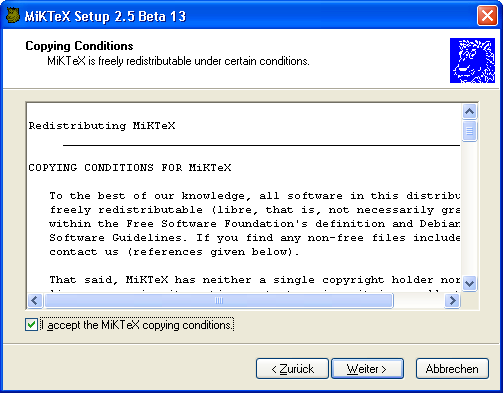
\includegraphics[width=7cm]{images/MiKTeX-install-01.png}
	\end{captionbeside}
	\label{fig:install01}
\end{figure}

\begin{figure}[hb]
	\begin{captionbeside}[Auswahl des Installationsmodus]{W�hle hier, ob nur Dein aktueller Nutzer oder alle am PC angemeldeten Nutzer MiKTeX nutzen k�nnen sollen. Letzteres ist empfehlenswert, damit es keine Probleme gibt.}[l]
		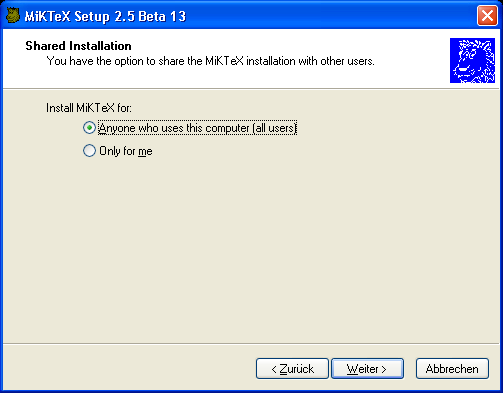
\includegraphics[width=7cm]{images/MiKTeX-install-02.png}
	\end{captionbeside}
	\label{fig:install02}
\end{figure}

\begin{figure}[hb]
	\begin{captionbeside}[Ziel der Installation w�hlen]{Hier kann das Ziel der Installation gew�hlt werden.}[l]
		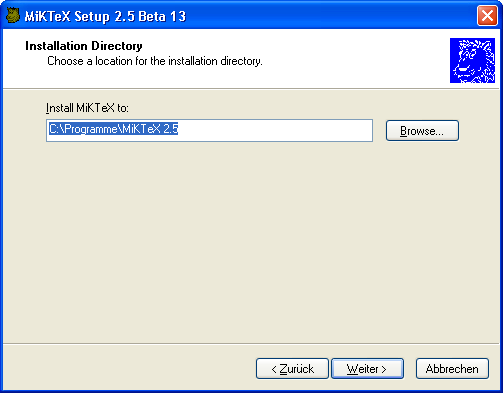
\includegraphics[width=7cm]{images/MiKTeX-install-03.png}
	\end{captionbeside}
	\label{fig:install03}
\end{figure}

\begin{figure}[hb]
	\begin{captionbeside}[Bevorzugtes Papierformat]{F�r den deutschen Sprachraum ist A4 ein sinnvoller Standard. Da Du f�r einzelne Dokumente das jeweilige Papierformat bestimmen kannst, gilt diese Einstellung nur f�r Dokumente ohne weitere Angabe.}[l]
		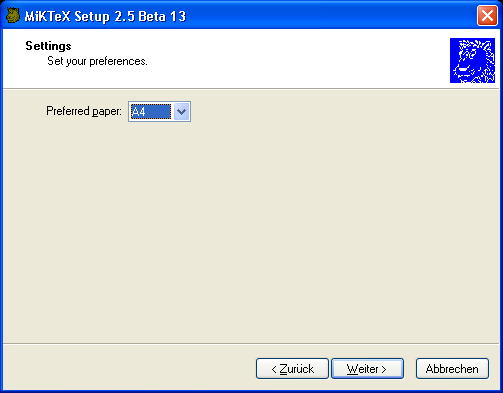
\includegraphics[width=7cm]{images/MiKTeX-install-04.png}
	\end{captionbeside}
	\label{fig:install04}
\end{figure}

\begin{figure}[th]
	\begin{captionbeside}{Der Best�tigungsscreen vor dem Start der eigentlichen Installation.}[l]
		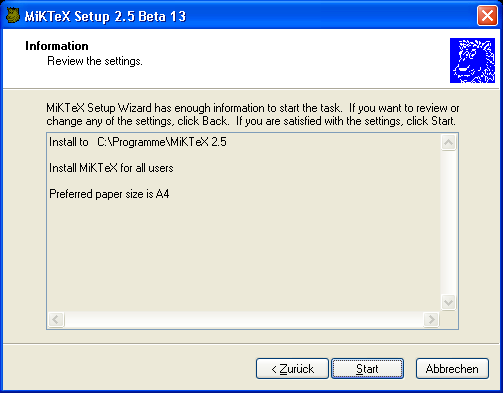
\includegraphics[width=7cm]{images/MiKTeX-install-05.png}
	\end{captionbeside}
	\label{fig:install06}
\end{figure}

\begin{figure}[th]
	\begin{captionbeside}[Die Pakete werden installiert]{Nun werden die einzelnen Pakete installiert.}[l]
		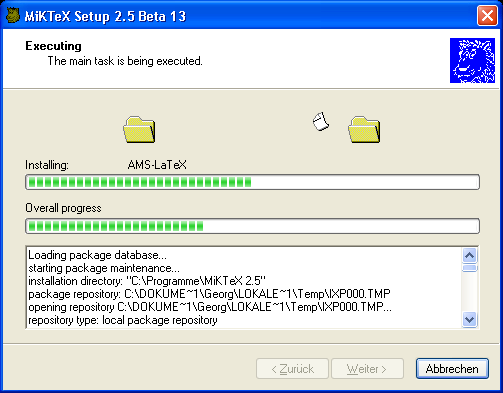
\includegraphics[width=7cm]{images/MiKTeX-install-07.png}
	\end{captionbeside}
	\label{fig:install07}
\end{figure}

\begin{figure}[th]
	\begin{captionbeside}[Das Ende des Setups]{Jetzt folgt noch ein kurzer Best�tigungsscreen und nach einem Klick auf \enquote{Close} wird das Setup beendet.}[l]
		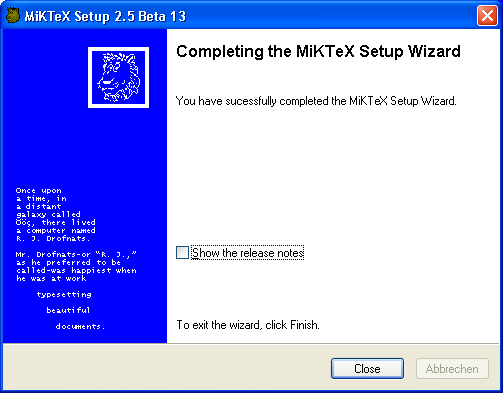
\includegraphics[width=7cm]{images/MiKTeX-install-08.png}
	\end{captionbeside}
	\label{fig:install08}
\end{figure}


\clearpage % Warten bis alle Floats ausgegeben sind.

\subsection{Herunterladen der Pakete}
\label{subsec:instpakete}

W�hrend der Benutzung von MiKTeX und TeXnicCenter wirst Du bei fehlenden Paketen gefragt, ob sie heruntergeladen werden sollen. Dies ist ein bequemer und minimalistischer Ansatz, da nur genau die Pakete installiert werden, die Du tats�chlich brauchst, und diese immer in der aktuellen Version aus dem Netz geladen werden. 

Alternativ Du kannst nat�rlich alle verf�gbaren Pakete auf einmal herunterladen -- z.B. sinnvoll, wenn Du nur vor�bergehend in der Uni breitbandig mit dem Internet verbunden bist und Festplattenplatz keinen Engpass darstellt (die allermeisten Pakete wirst Du nie verwenden, also den davon eingenommenen Platz verschwenden). Auf diese Weise stehen immer alle Pakete zur Verf�gung.

Wie du manuell einige oder alle Pakete installieren kannst, ist in den Abbildungen \ref{fig:install10} bis \ref{fig:install05b} beschrieben. 

\begin{figure}[hb]
	\begin{captionbeside}[MiKTeX Package Manager starten]{Rufe Start -- Programme -- MiKTeX -- Browse Packages auf. Der \enquote{MiKTeX Package Manager} wird gestartet. Du w�hlst die gew�nschten Pakete aus, indem Du die Steuerung-Tastste gedr�ckt h�lst und mit der Maus auf einzelne Pakete klickst, um mehrere verstreute zu markieren, bzw. indem Du die Umschalt-Tastste gedr�ckt h�lst, um mehrere benachbarte Bl�cke auszuw�hlen.)}[l]
		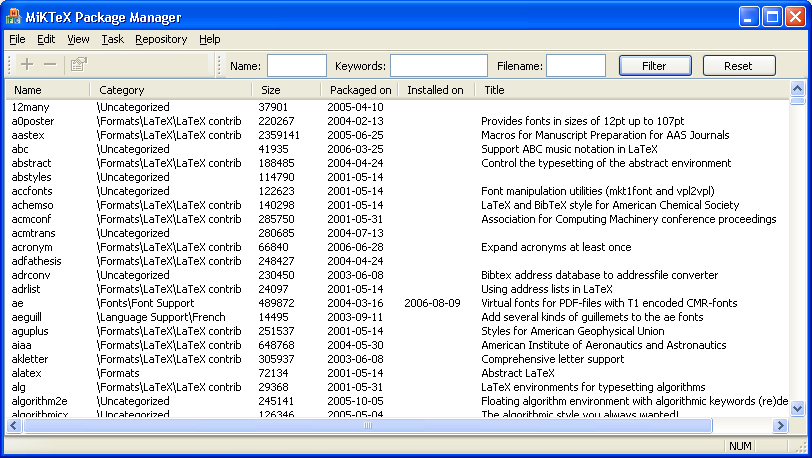
\includegraphics[width=7cm]{images/MiKTeX-packet-install-01.png}
	\end{captionbeside}
	\label{fig:install10}
\end{figure}

\begin{figure}[hb]
	\begin{captionbeside}[Auswahl der Pakete und Start der Installation]{Hast Du die gew�nschten Pakete ausgew�hlt, klickst Du auf das Plus-Icon bzw. gehst im Men� auf Task -- Install. Dieser Informationsbildschirm erscheint, den Du mit OK best�tigst.}[l]
		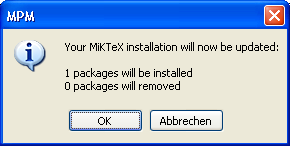
\includegraphics[width=7cm]{images/MiKTeX-packet-install-02.png}
	\end{captionbeside}
	\label{fig:install03b}
\end{figure}

\begin{figure}
	\begin{captionbeside}[Download]{Die Pakete werden aus dem Netz geladen und Dir Statusinformationen angezeigt. Klicke danach auf Close. Damit ist die Paketinstallation beendet.}[l]
		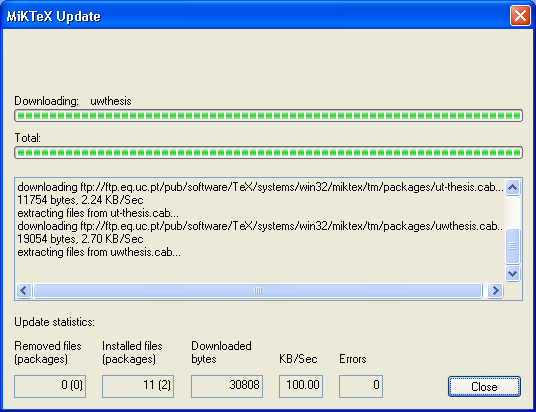
\includegraphics[width=7cm]{images/MiKTeX-packet-install-03.png}
	\end{captionbeside}
	\label{fig:install05b}
\end{figure}

\index{Installation!MiKTeX|)}

\clearpage % Warten bis alle Floats ausgegeben sind.

\section{Der Editor TeXnicCenter}
\index{Installation!TeXnicCenter|(}

Um \DMLLaTeX \ Dokumente einfach editieren zu k�nnen, bietet sich der Editor \enquote{TeXnicCenter}~\cite{TeXnicCenter} an. Dieser unterst�tzt einfache Navigation in der Dokumentstruktur, Projektverwaltung und einfachen Aufruf von \DMLLaTeX.

\subsection{Herunterladen von TeXnicCenter}

Auf der Webseite des TeXnicCenter Autors~\cite{TeXnicCenter} w�hlst du in der Navigation links \enquote{Download} an, und in der folgenden Liste, unter dem Punkt \enquote{End-User Downloads} z.\,B. \enquote{TeXnicCenter Setup, Version 1 Beta 7.01} aus. Vielleicht ist mittlerweile bereits eine neuere Version erschienen. Wichtig ist, dass du die \enquote{Binaries} in Form einer Setup \enquote{.exe} Datei herunterl�dst.

\subsection{Starten des Setups}

Starte das heruntergeladene Setup. Die Installation ist in den Abbildungen \ref{fig:install20} bis \ref{fig:install27} beschrieben.

\begin{figure}[hb]
	\begin{captionbeside}[Startscreen des Installationsassistenten]{Es erscheint der Installationsassistent.}[l]
		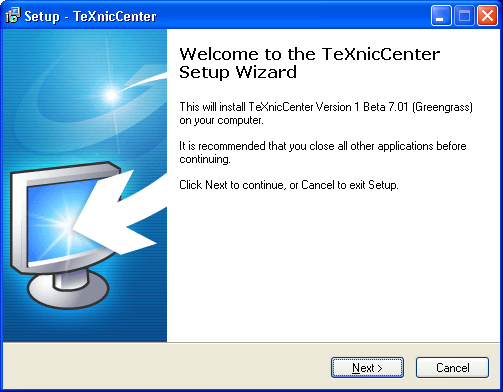
\includegraphics[width=7cm]{images/TeXnicCenter-install-01.png}
	\end{captionbeside}
	\label{fig:install20}
\end{figure}

\begin{figure}[hb]
	\begin{captionbeside}[Anzeige der GPL]{Die GNU Public License~\cite{GPL} mu� akzeptiert werden.}[l]
		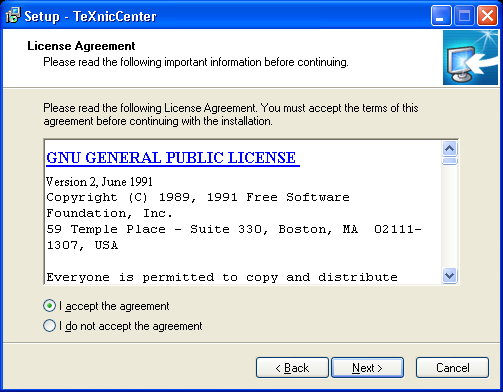
\includegraphics[width=7cm]{images/TeXnicCenter-install-02.png}
	\end{captionbeside}
	\label{fig:install21}
\end{figure}

\begin{figure}[hb]
	\begin{captionbeside}[Wahl des Installationsverzeichnisses]{Hier w�hlst du das Verzeichnis aus, in das der Editor installiert werden soll. Am Besten �bernimmst du die Vorgabe.}[l]
		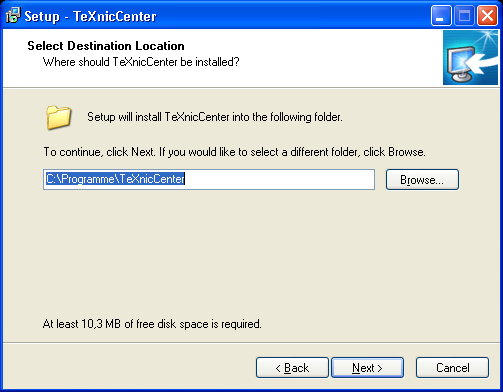
\includegraphics[width=7cm]{images/TeXnicCenter-install-03.png}
	\end{captionbeside}
	\label{fig:install22}
\end{figure}

\begin{figure}[hb]
	\begin{captionbeside}[Frage nach der Installationsart]{Jetzt wirst du nach der Installationsart gefragt. Hier w�hlst du \enquote{Typical} aus.}[l]
		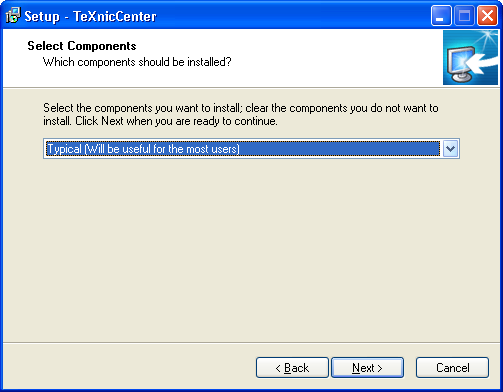
\includegraphics[width=7cm]{images/TeXnicCenter-install-04.png}
	\end{captionbeside}
	\label{fig:install23}
\end{figure}

\begin{figure}[hb]
	\begin{captionbeside}[Wahl des Namens im Startmen�]{Auch bei der Frage nach dem Namen des Eintrags ins Startmen� kannst du die Voreinstellung �bernehmen.}[l]
		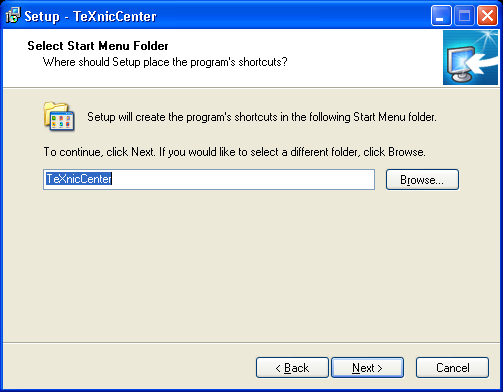
\includegraphics[width=7cm]{images/TeXnicCenter-install-05.png}
	\end{captionbeside}
	\label{fig:install24}
\end{figure}

\begin{figure}[thb]
	\begin{captionbeside}[Frage, ob ein Icon auf dem Desktop erzeugt werden soll]{Je nach Wunsch kannst du hier ein Icon auf dem Desktop und/oder einen Eintrag in das \enquote{Senden an} Kontextmen� erzeugen lassen.}[l]
		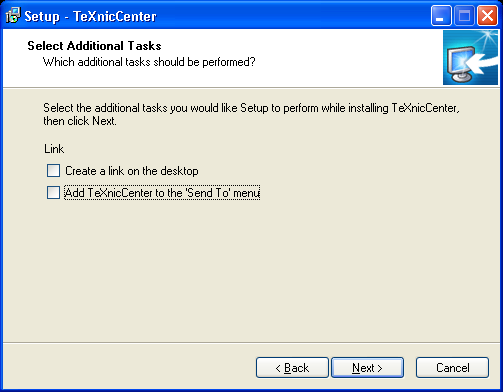
\includegraphics[width=7cm]{images/TeXnicCenter-install-06.png}
	\end{captionbeside}
	\label{fig:install25}
\end{figure}

\begin{figure}[thb]
	\begin{captionbeside}[Eine Zusammenfassung der Installation]{Jetzt folgt noch eine Zusammenfassung der Installationsangaben.}[l]
		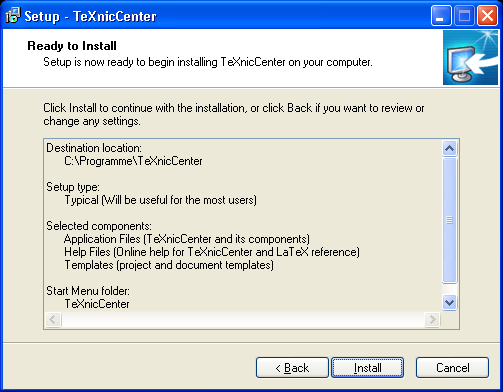
\includegraphics[width=7cm]{images/TeXnicCenter-install-07.png}
	\end{captionbeside}
	\label{fig:install26}
\end{figure}

\begin{figure}[thb]
	\begin{captionbeside}[TeXnicCenter ist installiert]{TeXnicCenter ist installiert.}[l]
		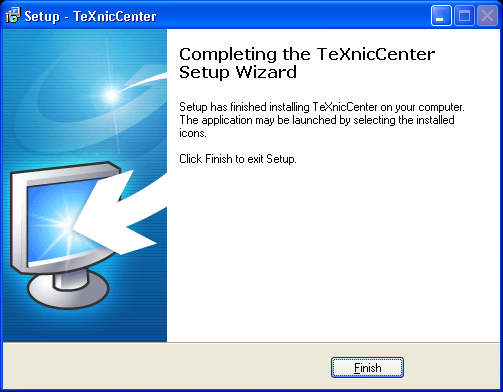
\includegraphics[width=7cm]{images/TeXnicCenter-install-08.png}
	\end{captionbeside}
	\label{fig:install27}
\end{figure}

\index{Installation!TeXnicCenter|)}

\clearpage % Warten bis alle Floats ausgegeben sind.


\section{Adobe Reader}
\index{Installation!Adobe Reader}

Jetzt solltest du noch die neuste Version des \enquote{Adobe Reader} herunterladen. Du ben�tigst mindestens die Version 5.0 (damals noch \enquote{Acrobat Reader}). Das Programm ist kostenlos und du solltest es nicht mit dem teuren \enquote{Adobe Acrobat} verwechseln, dem Programm, welches PDF-Dateien \emph{erzeugt}. Wir werden mit \DMLLaTeX \ unsere PDFs erzeugen.

Dazu gehst du auf die Webseite von Adobe~\cite{Adobe} und suchst nach einem Link \enquote{Download Adobe Reader} oder �hnlichem. Vielleicht findest du auch ein anklickbares \enquote{Get Adobe Reader} Icon. 

Du gelangst auf eine Seite mit einigen weiteren Informationen zum Adobe Reader. Weiter unten findest du drei Schritte zum Download.

Bei den Feldern im ersten Schritt w�hlst du Deutsch und dein Betriebssystem aus. Die Felder im zweiten Schritt kannst du leer lassen (empfohlen).

Nach dem Klick auf \enquote{Download} startet nach einigen Sekunden der Download von einem kleinen \enquote{Downloadmanager}. Nach dem Start von diesem Programm wird der Adobe Reader heruntergeladen und auf deinem System installiert.

\index{Installation|)}

%
% Diplomarbeit mit LaTeX
% ===========================================================================
% This is part of the book "Diplomarbeit mit LaTeX".
% Copyright (c) 2002, 2003, 2005 Tobias Erbsland, Andreas Nitsch
% See the file main.tex for copying conditions.
%

\chapter{Konfiguration}
\index{Konfiguration}

\section{MiKTeX}
\index{Konfiguration!MiKTeX}

Die \DMLLaTeX-Distribution \enquote{MiKTeX} musst du nicht konfigurieren. Es handelt sich dabei außer bei dem DVI-Betrachter um Kommandozeilentools. Du solltest nur den Editor TeXnicCenter einrichten (siehe dazu \ref{sec:KonfigurationTeXnicCenter}).

Du solltest jedoch mit dem \enquote{MiKTeX Update Wizard} alle Pakete der Distribution auf den neuesten Stand bringen. Wie du das machst, beschreibt die Hilfe zu MiKTeX ausführlich.\footnote{\enquote{User Guide}$\Rightarrow$\enquote{Maintenance}$\Rightarrow$\enquote{Installing Updates}}

\section{TeXnicCenter}
\label{sec:KonfigurationTeXnicCenter}
\index{Konfiguration!TeXnicCenter}

\subsection{TeXnicCenter für die Verwendung mit MiKTeX konfigurieren}

Nach dem ersten Start erscheint der Einrichtungsassistent. Falls du diesen bereits abgebrochen hast, kann man ihn über das Menü \enquote{Ausgabe}, \enquote{Ausgabeprofile definieren...} und dort in dem Dialog \enquote{Assistent} links unten erneut aufrufen. Doch wie schon gesagt, der Assistent startet normalerweise beim ersten Start vom TeXnicCenter automatisch.

\begin{figure}[hb]
	\begin{captionbeside}[Start des Konfigurations-Assistenten]{Der Konfigurationsassistent  startet mit diesem Screen.}[l]
		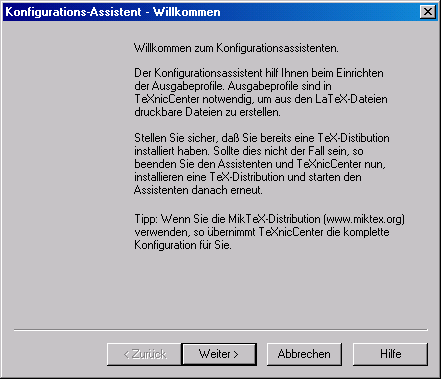
\includegraphics[width=7cm]{images/konfiguration01.png}
	\end{captionbeside}
	\label{fig:konfiguration01}
\end{figure}

\begin{figure}[hb]
	\begin{captionbeside}[Frage, für welche Distribution TeXnicCenter eingerichtet werden soll]{Hier teilt der Installations"=Assistent mit, dass die installierte MiKTeX"=Distribution erkannt wurde und fragt, ob er den Editor mit dieser \DMLLaTeX"=Distribution konfigurieren soll. Du wählst natürlich \enquote{Ja}.}[l]
		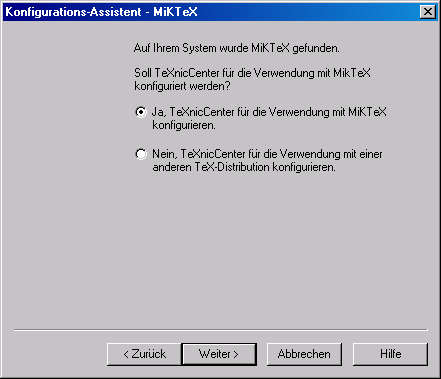
\includegraphics[width=7cm]{images/konfiguration02.png}
	\end{captionbeside}
	\label{fig:konfiguration02}
\end{figure}

\begin{figure}[ht]
	\begin{captionbeside}[Optionale Eingabe eines Postscript Betrachters]{Jetzt wirst du nach einem Programm zur PostScript-Betrachtung gefragt. Hier lässt du alle Felder leer.}[l]
		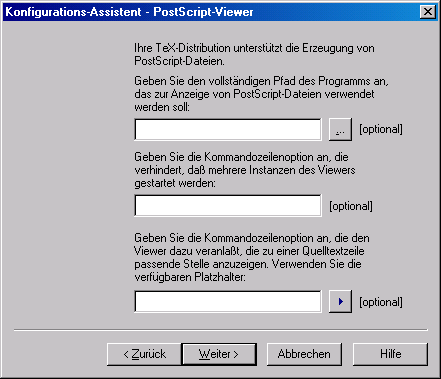
\includegraphics[width=7cm]{images/konfiguration03.png}
	\end{captionbeside}
	\label{fig:konfiguration03}
\end{figure}

\begin{figure}[ht]
	\begin{captionbeside}[Anzeige der drei generierten Profile]{Der TeXnicCenter-Assistent teilt dir mit, dass er drei Profile generieren wird. Ein DVI-, ein PostScript- und ein PDF-Profil. Wir werden nur das PDF-Profil verwenden.}[l]
		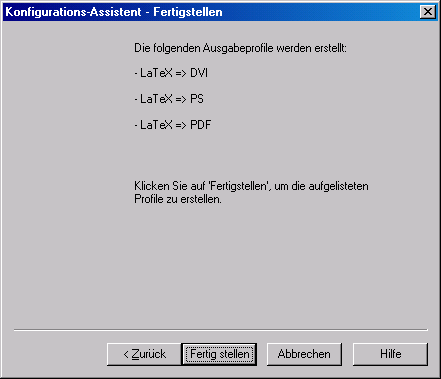
\includegraphics[width=7cm]{images/konfiguration04.png}
	\end{captionbeside}
	\label{fig:konfiguration04}
\end{figure}

\clearpage % Warten auf alle Floats

\subsection{Die Rechtschreibprüfung}
\index{Rechtschreibprufung@Rechtschreibprüfung}

Ein sehr nützliches Feature, welches dir TeXnicCenter bietet, ist die Rechtschreibprüfung. Wähle dazu im Menü \emph{Extras} den Punkt \emph{Optionen} aus. In dem Dialog, der sich öffnet, wählst du den Reiter \emph{Rechtschreibung} aus. Dort kannst du die verschiedenen Optionen der Rechtschreibprüfung einstellen, wie du in Abbildung \ref{fig:rechtschreibung} siehst.

\begin{figure}
	\centering
		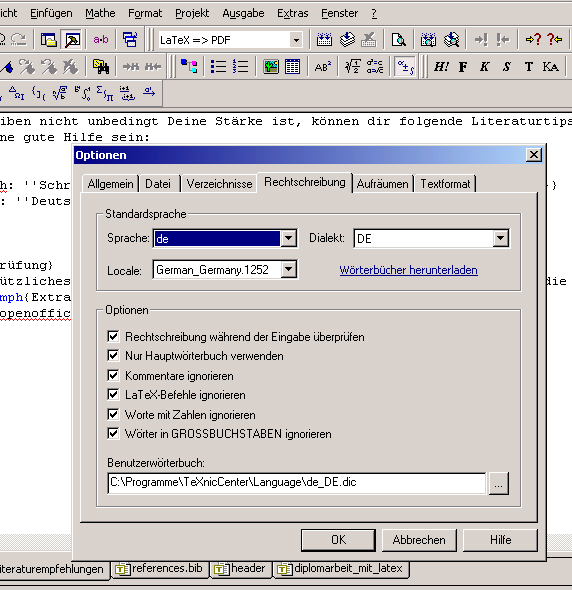
\includegraphics[width=0.60\textwidth]{images/rechtschreibung.png}
	\caption{Konfigurationsmöglichkeiten der Rechtschreibprüfung}
	\label{fig:rechtschreibung}
\end{figure}

Falls eine gewünschte Sprache fehlt, findest du Wörterbücher weiterer Sprachen unter
\urlindent{https://extensions.services.openoffice.org/dictionaries}
zum kostenlosen Download. Entpacke die in der heruntergeladenen ZIP"=Datei enthaltenen Dateien in das Unterverzeichnis \enquote{Language} deiner TeXnicCenter"=Installation, normalerweise ist das:

\verb|C:\Programme\TeXnicCenter\Language|.

%
% Diplomarbeit mit LaTeX
% ===========================================================================
% This is part of the book "Diplomarbeit mit LaTeX".
% Copyright (c) 2002-2005 Tobias Erbsland, Andreas Nitsch
% See the file diplomarbeit_mit_latex.tex for copying conditions.
%

\chapter{Grundlagen}
\label{sec:grundlagen}
\index{Grundlagen|(}

\DMLLaTeX \ ist einfacher zu erlernen, als du vielleicht denkst. Anders als grafische Tools, welche WYSIWYG\footnote{What You See Is What You Get} bieten (wollen), beschreibst du �hnlich wie bei HTML die Struktur deines Dokuments in einer speziellen Sprache. Danach \enquote{kompilierst} du das Dokument und erzeugst dadurch das fertige Dokument, zum Beispiel eine PDF-Datei.


\section{Das erste kleine LaTeX"=Dokument}

\subsection{Erstellen eines neuen Projekts}
\label{sec:erstellenneuesprojekt}
\index{Erstellen!Projekt}\index{Projekt erstellen}\index{Neues Projekt}

Starte jetzt im TeXnicCenter ein neues Projekt. Dazu gehst du auf \enquote{Datei}, dort auf \enquote{Neues Projekt...} (siehe dazu Abbildung \ref{fig:beispiel1_01}).

\begin{figure}[ht]
	\begin{center}
		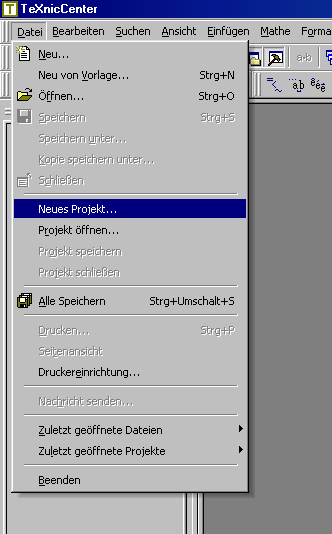
\includegraphics[width=3cm]{images/beispiel1_01.png}
	\end{center}
	\caption{Ausw�hlen von \enquote{Neues Projekt...} �ber das Men�}
	\label{fig:beispiel1_01}
\end{figure}


Ein Dialogfenster �ffnet sich, in dem du den Projekttyp\index{Projekttyp} ausw�hlen kannst. Es steht nur \enquote{Leeres Projekt} zur Verf�gung. Klicke dieses Icon an und w�hle rechts das Basisverzeichnis aus. F�r jedes \DMLLaTeX"=Dokument wird ein neues Unterverzeichnis in diesem Basisverzeichnis erstellt.

Ich empfehle dir Folgendes: Lege auf deinem Datenlaufwerk (z.\,B. M:\textbackslash ) ein Verzeichnis \enquote{Dokumente} an. Darin erstellst du z.\,B. noch ein Unterverzeichnis \enquote{LaTeX}.

Gib dieses Verzeichnis nun als \enquote{Basisverzeichnis} im Projektdialog an.

Jetzt kannst du einen Projektnamen eingeben. Gib z.\,B. \enquote{Beispiel1} als Projektnamen ein. W�hrend du den Projektnamen eingibst, siehst du, dass das Basisverzeichnis im unteren Feld um diesen Projektnamen erweitert wird. Siehe dazu Abbildung \ref{fig:beispiel1_02}.

\begin{figure}[ht]
	\begin{center}
		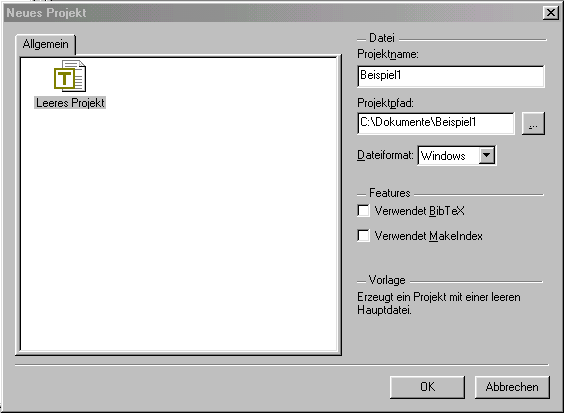
\includegraphics[width=5cm]{images/beispiel1_02.png}
	\end{center}
	\caption{Der Dialog f�r ein neues Projekt}
	\label{fig:beispiel1_02}
\end{figure}

Wenn du den Projektnamen eingegeben hast, klickst du auf \enquote{Ok}. Jetzt wird das neue Projekt erstellt. Dazu wird das Unterverzeichnis \enquote{Beispiel1} erstellt, und darin die Datei \enquote{Beispiel1.tcp}. Dies ist die Projektdatei.

Weiter wird eine neue Datei \enquote{Beispiel1.tex} erstellt. Dies ist unsere \DMLLaTeX-Datei.

\subsection{Erstes Beispiel}
\label{sec:erstesbeispiel}

Schreibe jetzt folgende Zeilen in die leere Datei:

\lstinputlisting[caption=Beispiel1.tex, label=lst:beispiel01, frame=tb]%
	{listings/beispiel01.tex}

Die Zeilen 5--11 sind der Kopfbereich der Datei. Hier definieren wir Folgendes:

\begin{description}
\item[Zeile 5] Der Befehl \texttt{\textbackslash documentclass}\index{documentclass@\texttt{\textbackslash documentclass}} definiert unsere Dokumentklasse\index{Dokumentklasse}. Wir verwenden hier die Klasse \enquote{scrartcl}, welche f�r kleinere Artikel gedacht ist. Neben der \KOMAScript{} Klasse \enquote{scrartcl} gibt es z.\,B. noch \enquote{scrbook}, \enquote{scrreprt}, \enquote{scrlettr} und andere weniger �bliche.
\item[Zeile 6] Mit dem Paket \enquote{ngerman}\index{Paket!ngerman}, welches wir hier laden, werden verschiedene Titel ins Deutsche �bersetzt. So z.\,B. \enquote{Table of Contents} in \enquote{Inhaltsverzeichnis}. Zudem aktiviert dieses Paket die korrekte Silbentrennung f�r die neue deutsche Rechtschreibung.

Falls du lieber die alte deutsche Rechtschreibung verwenden m�chtest, dann solltest du statt dem Paket \enquote{ngerman} das Paket \enquote{german}\index{Paket!german} einbinden.
\item[Zeile 7] \enquote{inputenc}\index{Paket!inputenc} binden wir ein, damit die deutschen Zeichen �, �, �, �, �, � und � automatisch erkannt werden und wir diese nicht als \enquote{''a} usw. schreiben m�ssen.
\item[Zeile 8] Das Paket \enquote{fontenc} mit der Option \enquote{T1}, �ndert die Fontkodierung auf das \enquote{T1} Format. %TODO: Erl�uterung, wozu dieses gut sein soll

Normalerweise verwendet \DMLLaTeX \ Schriftarten mit einem Umfang von 128 Zeichen. Darin sind z.\,B. keine Umlaute oder Buchstaben mit Akzenten enthalten. Diese werden jeweils aus dem Buchstaben und Akzent zusammengesetzt. Also \enquote{a} und \enquote{\textasciicircum} ergibt \enquote{�}.

Mittlerweile stehen f�r die meisten Schriften in den \DMLLaTeX-Distributionen erweiterte \enquote{europ�ische} Versionen zur Verf�gung (In der \enquote{T1-Codierung}). Diese Schriften enthalten bis zu 256 Zeichen. Dort sind auch Umlaute und akzentuierte Zeichen vorgefertigt enthalten. Das f�hrt zu einer h�heren typographischen Qualit�t der Dokumente und l�st auch einige Probleme mit der Silbentrennung.
\item[Zeile 10 und 11] Hier definieren wir den Titel\index{Dokumenttitel} und den Autor\index{Autor} des Dokuments.
\end{description}

Die Zeilen 13--23 bilden dann den eigentlichen Inhalt des Dokuments. Der Dokumentinhalt wird immer durch die Zeilen \enquote{\textbackslash begin\{document\}} und \enquote{\textbackslash end\{document\}} eingeschlossen.

\begin{description}
\item[Zeile 15] Mit diesem Befehl wird der Titel\index{Titel erstellen}\index{Erstellen!Titel} unseres Dokumentes erstellt. Die n�tigen Angaben dazu liefern die Zeilen 11 und 12. Wird nirgendwo ein festes Datum\index{Festes Datum}\index{Datum!fest} angegeben, wird das aktuellen Datum\index{Aktuelles Datum}\index{Datum!aktuelles} genommen. In unserem Fall erscheint dann das aktuelle Datum auf der Titelseite.
\item[Zeile 17] \texttt{\textbackslash tableofcontents}\index{tableofcontents@\texttt{\textbackslash tableofcontents}} f�gt an dieser Stelle das Inhaltsverzeichnis\index{Inhaltsverzeichnis} ein. Wir m�ssen uns in keiner Weise um das Inhaltsverzeichnis k�mmern. Es wird automatisch aus den �berschriften generiert.
\item[Zeile 19] Hier defininieren wir die erste �berschrift.
\item[Zeile 21] Ein kleiner Absatz mit Text rundet unser kleines Beispieldokument ab.
\end{description}

\subsection{Einstellen des Ausgabeformats}
\index{Ausgabeformats}\index{Ausgabeformat einstellen}\index{Einstellen!Ausgabeformat}

Kontrolliere vor dem ersten Kompilieren, ob du als Ausgabeformat \enquote{PDF} eingestellt hast. Du siehst diese Einstellung in der Symbolleiste (siehe dazu Abbildung \ref{fig:beispiel1_03}).

\begin{figure}[ht]
	\begin{center}
		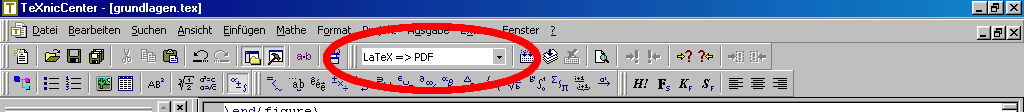
\includegraphics[width=\linewidth]{images/beispiel1_03.png}
	\end{center}
	\caption{Einstellen des Ausgabeformats}
	\label{fig:beispiel1_03}
\end{figure}

Stelle dieses Pulldownmen� auf \enquote{LaTeX => PDF} ein. Ein anderer Weg ist �ber das Men�: \enquote{Ausgabe} $\Rightarrow$ \enquote{Aktives Ausgabeprofil w�hlen...}.

\subsection{Speichern und Kompilieren}
\index{Speichern}\index{Kompilieren}

Speichere die Datei jetzt mit \enquote{Ctrl+S} oder �ber das Men� \enquote{Datei} $\Rightarrow$ \enquote{Speichern} oder durch einen Klick auf das Diskettensymbol in der Symbolleiste.

Jetzt kannst du den Kompiliervorgang mit der Taste \enquote{F7} starten oder �ber das Men� \enquote{Ausgabe} $\Rightarrow$ \enquote{Projekt compilieren} oder auch �ber die Symbolleiste.

Im Statusbereich laufen jetzt diverse Meldungen vorbei. Nach einigen Sekunden oder Minuten, je nachdem, wie schnell dein Computer ist, ist der Kompiliervorgang vorbei. Im Statusfenster siehst du z.\,B. folgende Ausgabe:

\begin{lstlisting}
LaTeX-Ergebnis: 0 Fehler, 1 Warnung(en), 0 zu volle/leere Box(en), 1 Seite(n)
\end{lstlisting}

Es sollten beim Kompiliervorgang keine Fehler aufgetreten sein. Hast du trotzdem Fehler, kontrollierst du am besten noch einmal deinen Text. Vielleicht haben sich ja Tippfehler eingeschlichen.

Mit der Taste \enquote{F9} springst du von einem Fehler zum n�chsten. Dabei springt der Cursor an die Stelle in deinem Dokument, an welcher der Fehler \emph{vermutet} wird. Nat�rlich kann sich der Fehler auch einige Zeilen davor oder danach befinden.

Sind alle Fehler behoben, kannst du mit \enquote{F5} oder �ber das Men� \enquote{Ausgabe} $\Rightarrow$ \enquote{Ausgabe betrachten} das fertige Dokument betrachten. Dazu wird der Adobe Reader gestartet und das fertige Dokument angezeigt (siehe dazu Abbildung \ref{fig:beispiel1_04}).

\begin{figure}[ht]
	\begin{center}
		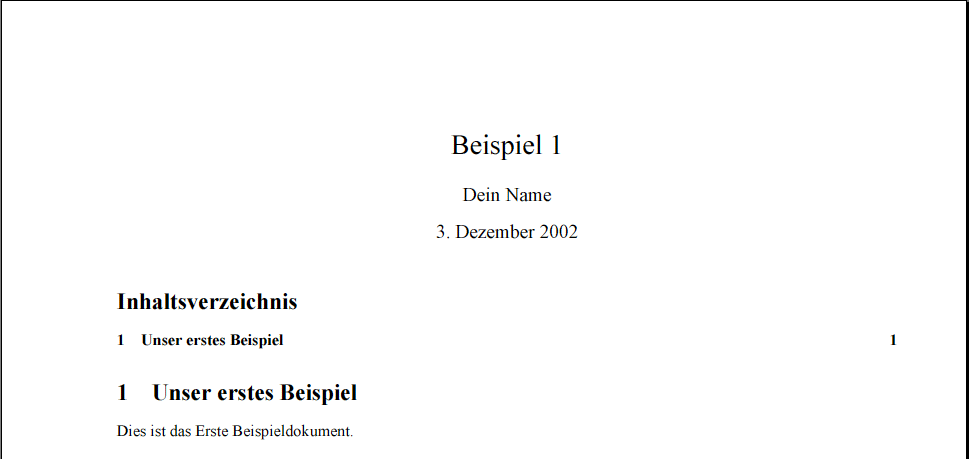
\includegraphics[width=\linewidth]{images/beispiel1_04.png}
	\end{center}
	\caption{Das fertige Beispieldokument}
	\label{fig:beispiel1_04}
\end{figure}

Den Adobe Reader musst du w�hrend der Arbeit mit dem TeXnicCenter nicht mehr schlie�en. Wenn du �nderungen am Dokument machst und dieses �bersetzen l�sst, kannst du mit \enquote{F5} die Anzeige im bereits ge�ffneten Adobe Reader einfach auffrischen lassen. Dies geht auch wesentlich schneller, als wenn jedesmal der Adobe Reader gestartet werden m�sste.
%TODO: Hier w�re ein Hinweis auf die Vorschau im DVI-Viewer sch�n -> hier automatischer Refresh

\index{Grundlagen|)}

\section{Sonderzeichen}
\index{Sonderzeichen}\label{Sonderzeichen}

Alle \DMLLaTeX \ Befehle beginnen mit einem \enquote{Backslash}, zudem gibt es einige Sonderzeichen welche du nicht direkt verwenden darfst. Hier das Beispiel eines
\DMLLaTeX \ Befehls:

\begin{lstlisting}
	\textbackslash
\end{lstlisting}

Die Sonderzeichen, welche du nicht direkt verwenden darfst, liste ich hier kurz auf. Sp�ter erf�hrst du, wie man diese Sonderzeichen in den Text einbauen kann und welchen Zweck sie haben. Verzichte am Anfang einfach auf diese Zeichen.

\begin{lstlisting}
	% # $ & ~ _ ^ \ { } "
\end{lstlisting}

\section{Kommentare mit \%}
\index{Kommentare}\index{Prozentzeichen}

Das Prozentzeichen (\%) wird f�r Kommentare innerhalb deiner Datei verwendet. Damit kannst du f�r dich Anmerkungen machen und Dinge kommentieren. 

Wenn du spezielle Pakete in deinem \DMLLaTeX \ Dokument einbindest, solltest du z.\,B. mit einem kurzen Kommentar beschreiben, was dieses Paket macht.

Falls du ein Prozentzeichen in deinen Text einbauen m�chtest, musst du einen Backslash vor das Prozentzeichen setzen.

\begin{lstlisting}
%
% Ein Kommentar
%

Hier mit 100\% ein Prozentzeichen
\end{lstlisting}




%
% Diplomarbeit mit LaTeX
% ===========================================================================
% This is part of the book "Diplomarbeit mit LaTeX".
% Copyright (c) 2002-2005 Tobias Erbsland, Andreas Nitsch
% See the file diplomarbeit_mit_latex.tex for copying conditions.
%

\chapter{Text formatieren}
\index{Formatieren|(}

\DMLLaTeX \ kennt verschiedenste Arten, auf die ein Text formatiert und strukturiert werden kann. Ich zähle hier nur die wichtigsten mit kleinen Beispielen auf.

\section{Absätze und Zeilenumbrüche}

Es spielt keine Rolle, wie genau du den Text innerhalb deines Dokuments formatierst. Die folgenden beiden Listings ergeben also dasselbe Resultat:

\begin{lstlisting}
Ein Beispieltext auf einer einzelnen Zeile.
\end{lstlisting}

\begin{lstlisting}
Ein Beispieltext
auf einer
einzelnen Zeile.
\end{lstlisting}

Dabei ignoriert \DMLLaTeX \ überflüssige Leerzeichen und Zeilenumbrüche. Du kannst den Text in deiner Datei so formatieren, dass er für dich zum Editieren übersichtlich ist.

\subsection{Absätze}
\index{Formatieren!Absaetze@Absätze}
\index{Absatz}

Um einen Absatz zu erzeugen, fügst du einfach mindestens eine Leerzeile zwischen zwei Textstellen in dein Dokument ein:

\begin{lstlisting}
Dies ist der erste Absatz von
diesem Dokument.

Das ist der zweite.
\end{lstlisting}

\DMLLaTeX \ formatiert normalerweise neue Absätze so, dass die erste Zeile des neuen Absatzes ein wenig eingerückt wird. Dies entspricht den amerikanischen Absatzregeln. \index{Absatzregeln}\index{Europaeische Absaetze@Europäische Absätze}Um europäische Absätze zu erzeugen, existieren in den \KOMAScript-Dokumentklassen verschiedenste Optionen.

\begin{itemize}
	\item parskip\index{parskip}\index{Dokumentklasse!Optionen}
	\item parskip*
	\item parskip+
	\item parskip-
	\item halfparskip\index{halfparskip}
	\item halfparskip*
	\item halfparskip+
	\item halfparskip-
	\item parindent\index{parindent}
\end{itemize}

Voreingestellt ist \enquote{parindent}. Alle Optionen, welche mit \enquote{parskip} beginnen, erzeugen eine ganze Zeile Abstand zwischen zwei Absätzen. Die Optionen, welche mit \enquote{halfparskip} beginnen, erzeugen eine halbe Zeile Zwischenraum. Der Stern, das Plus und Minus steuern u.a., wieviel Leerraum in der letzten Zeile eines Absatzes freibleiben soll.

Wie du diese Optionen bei der Dokumentklasse setzt, findest du in Kapitel~\ref{sec:globaleoptionen}. Weitere Informationen zu diesen Optionen findest du im \enquote{scrguide}, welchen du in \cite{KOMA} oder lokal auf deiner Festplatte im \enquote{doc} Verzeichnis deiner MiKTeX"=Distribution findest (z.\,B. unter C:\textbackslash texmf\textbackslash doc\textbackslash latex\textbackslash koma-script).

\subsection{Zeilenumbrüche}
\index{Formatieren!Zeilenumbrueche@Zeilenumbrüche}
\index{Zeilenumbruch}

Einen einfachen Zeilenumbruch kannst du mit einem doppelten Backslash erzeugen. Dabei wird die Zeile genau an dieser Stelle umbrochen. Zeilenumbrüche sollten nur in speziellen Fällen verwendet werden, wie z.\,B. bei Adressen, in Tabellen oder ähnlichen Situationen.

\begin{lstlisting}
Hans Muster \\
Mustergasse 12 \\
1234 Musterhausen
\end{lstlisting}

\section{Überschriften}
\index{Formatieren!Ueberschriften@Überschriften}
\index{Ueberschriften@Überschriften}

Überschriften bilden die Struktur des Dokuments. Es existieren folgende Überschriftstypen:
\index{chapter@\texttt{\textbackslash chapter}}
\index{section@\texttt{\textbackslash section}}
\index{subsection@\texttt{\textbackslash subsection}}
\index{subsubsection@\texttt{\textbackslash subsubsection}}
\index{paragraph@\texttt{\textbackslash paragraph}}
\index{subparagraph@\texttt{\textbackslash subparagraph}}

\begin{enumerate}
	\item \texttt{\textbackslash chapter\{Kapitel\}}
	\item \texttt{\textbackslash section\{Abschnitt\}}
	\item \texttt{\textbackslash subsection\{Unterabschnitt\}}
	\item \texttt{\textbackslash subsubsection\{Unter-Unterabschnitt\}}
	\item \texttt{\textbackslash paragraph\{Absatz\}}
	\item \texttt{\textbackslash subparagraph\{Unter-Absatz\}}
\end{enumerate}

Der Befehl \texttt{\textbackslash chapter} existiert nur in den Dokumentklassen \enquote{scrbook} und \enquote{scrreprt}. Weiterhin gibt es noch den Befehl \texttt{\textbackslash part}. Mehr zu Dokumentklassen findest du in Kapitel~\ref{sec:dokumentklassen}.

Zu jedem Überschriftstyp existiert noch eine Form mit einem \enquote{*}:

\begin{enumerate}
	\item \texttt{\textbackslash chapter*\{Kapitel\}}
	\item \texttt{\textbackslash section*\{Abschnitt\}}
	\item \texttt{\textbackslash subsection*\{Unterabschnitt\}}
	\item \texttt{\textbackslash subsubsection*\{Unter-Unterabschnitt\}}
	\item \texttt{\textbackslash paragraph*\{Absatz\}}
	\item \texttt{\textbackslash subparagraph*\{Unter-Absatz\}}
\end{enumerate}

Diese Befehle generieren analog zu den ersten Befehlen die entsprechende Überschrift, jedoch ohne Nummerierung. Zudem taucht diese Überschrift nicht im Inhaltsverzeichnis auf.




\section{Textstellen hervorheben}
\index{Formatieren!Hervorheben}

Einzelne Wörter oder Textteile können \emph{hervorgehoben} werden. Dies machst du mit dem Befehl \texttt{\textbackslash emph}:

\begin{lstlisting}
Einzelne Wörter oder Textteile können \emph{hervorgehoben} werden.
\end{lstlisting}

Neben dieser einfachen Her\-vor\-he\-bung kannst du Wörter auch \textbf{fett}\index{Fett}\index{Formatieren!Fett}\index{textbf@\texttt{\textbackslash textbf}}, \textit{kursiv}\index{Kursiv}\index{Formatieren!Kursiv}\index{textit@\texttt{\textbackslash textit}} oder\\ \texttt{monospaced}\index{Monospaced}\index{Formatieren!Monospaced}\index{Feste Zeichenbreite}\index{texttt@\texttt{\textbackslash texttt}} setzen lassen:

\begin{lstlisting}
\textbf{fett}, \textit{kursiv} oder \texttt{monospaced}.
\textbf{Ganze Textzeile fett}
\end{lstlisting}

Du solltest jedoch für eine einfache Hervorhebung immer den \texttt{\textbackslash emph} Befehl verwenden. Die Formatierung des \texttt{\textbackslash emph} Befehls lässt sich nachtränglich beliebig neu definieren.

Beachte auch dass fetter Text die Aufmerksamkeit des Lesers auf die so markierte Stelle lenkt. Damit unterbrichst du den normalen Lesefluss. Verwendest du viele fett markierte Textstellen, wird das Lesen deines Dokuments zur Qual.

\section{Listen und Aufzählungen}
\index{Listen|(}\index{Aufzaehlungen@Aufzählungen|(}

Es gibt verschiedenste Listen und Aufzählungen in \DMLLaTeX. Hier zeige ich die wichtigsten davon:

\subsection{Einfache Aufzählung}
\index{Aufzaehlungen@Aufzählungen!einfache}\index{Einfache Aufzaehlung@einfache Aufzählung}

Eine einfache Aufzählung erstellst du folgendermaßen:

\begin{lstlisting}
\begin{itemize}
	\item Der erste Punkt.
	\item Der zweite Punkt in der Liste.
	\item Noch ein weiterer Punkt.
\end{itemize}
\end{lstlisting}

Und so sieht das ganze danach aus:

\begin{itemize}
	\item Der erste Punkt.
	\item Der zweite Punkt in der Liste.
	\item Noch ein weiterer Punkt.
\end{itemize}

\subsection{Nummerierte Aufzählung}
\index{Aufzaehlungen@Aufzählungen!nummerierte}\index{Nummerierte Aufzaehlung@nummerierte Aufzählung}

Eine nummerierte Aufzählung erstellst du folgendermaßen:

\begin{lstlisting}
\begin{enumerate}
	\item Ein nummerierter Punkt.
	\item Der zweite nummerierte Punkt.
	\item Noch ein dritter nummerierter Punkt.
\end{enumerate}
\end{lstlisting}

Und so sieht das ganze fertig aus:

\begin{enumerate}
	\item Ein nummerierter Punkt.
	\item Der zweite nummerierte Punkt.
	\item Noch ein dritter nummerierter Punkt.
\end{enumerate}

\subsection{Verschachtelte Aufzählungen}
\index{Aufzaehlungen@Aufzählungen!verschachtelte}\index{Verschachtelte Aufzaehlungen@verschachtelte Aufzählungen}

Diese Aufzählungstypen lassen sich beliebig verschachteln:

\begin{lstlisting}
\begin{enumerate}
	\item Ein nummerierter Punkt.
	\item Der zweite nummerierte Punkt.
	\begin{enumerate}
		\item Ein nummerierter Punkt.
		\item Der zweite nummerierte Punkt.
		\item Noch ein dritter nummerierter Punkt.
	\end{enumerate}
	\item Noch ein dritter nummerierter Punkt.
\end{enumerate}
\end{lstlisting}

Und so sieht das ganze fertig aus:

\begin{enumerate}
	\item Ein nummerierter Punkt.
	\item Der zweite nummerierte Punkt.
	\begin{enumerate}
		\item Ein nummerierter Punkt.
		\item Der zweite nummerierte Punkt.
		\item Noch ein dritter nummerierter Punkt.
	\end{enumerate}
	\item Noch ein dritter nummerierter Punkt.
\end{enumerate}


\subsection{Beschreibungslisten}
\index{Listen!Beschreibungslisten}\index{Beschreibungslisten}

Eine weitere Form einer Aufzählung ist die Beschreibungsliste. Hier ist ein Beispiel einer Beschreibungsliste:

\begin{lstlisting}
\begin{description}
	\item[Apfel] Eine Frucht die meistens auf großen Bäumen wächst,
		welche man ernten kann und welche ganz lecker schmeckt.
		Teilweise ist auch ein Wurm drin. Da dies ein längerer Satz ist,
		erkennt man, wie weitere Zeilen mit einem fixen Abstand 
		umbrochen werden.
	\item[Wurm] Ist teilweise im Apfel drin.
		Um auch hier den Abstand beim Umbruch in eine neue 
		Zeile zu sehen, schreibe ich einen längeren Satz.
		Mit einem bisschen Glück ist die Beschreibung hier
		länger als eine Zeile.
	\item[Birne] Siehe dazu \emph{Apfel}, nur mit anderer
		Form und Geschmack.
\end{description}
\end{lstlisting}

Und so sieht das ganze fertig aus:

\begin{description}
	\item[Apfel] Eine Frucht die meistens auf großen Bäumen wächst,
		welche man ernten kann und welche ganz lecker schmeckt.
		Teilweise ist auch ein Wurm drin. Da dies ein längerer Satz ist,
		erkennt man, wie weitere Zeilen mit einem fixen Abstand 
		umbrochen werden.
	\item[Wurm] Ist teilweise im Apfel drin.
		Um auch hier den Abstand beim Umbruch in eine neue Zeile zu sehen,
		schreibe ich einen längeren Satz. Mit einem bisschen Glück ist die
		Beschreibung hier länger als eine Zeile.
	\item[Birne] Siehe dazu \emph{Apfel}, nur mit anderer Form und Geschmack.
\end{description}

\index{Listen|)}\index{Aufzaehlungen@Aufzählungen|)}
\index{Formatieren|)}

%\include{chapters/querverweise}
%
% Diplomarbeit mit LaTeX
% ===========================================================================
% This is part of the book "Diplomarbeit mit LaTeX".
% Copyright (c) 2002-2005 Tobias Erbsland, Andreas Nitsch
% See the file diplomarbeit_mit_latex.tex for copying conditions.
%

\chapter{Dokumentklassen}
\label{sec:dokumentklassen}
\index{Dokumentklasse}\index{documentclass@\texttt{\textbackslash documentclass}|textbf}

Das grunds�tzliche Layout eines \DMLLaTeX-Dokuments wird durch verschiedene Dokumentklassen bestimmt. Es existieren verschiedenste Pakete, welche weitere Dokumentklassen zu den Standardklassen hinzuf�gen.

Eine interessante Erweiterung von \DMLLaTeX, welche f�r dieses Dokument verwendet wurde, ist \KOMAScript~\cite{KOMA}\index{KOMA-Script@\KOMAScript}. Wir beschreiben daher von Anfang an den Aufbau mit den \KOMAScript-Klassen. Sie bieten eine Vielzahl von Optionen und einer Anpassung der Standardklassen an die europ�ische Typographie.

Hier beschreibe ich die drei am h�ufigsten verwendeten Klassen und die wichtigsten Unterschiede zwischen diesen.

\section{Generelle Syntax, um die Dokumentklasse zu definieren}

Pro Dokument kann nur eine Dokumentklasse definiert werden. Diese Deklaration muss der erste Befehl in deinem \DMLLaTeX-Dokument, bzw. im Header, sein. Die generelle Syntax, um eine Dokumentklasse zu w�hlen, ist folgende:

\begin{lstlisting}
\documentclass[Optionen]{Name der Klasse}
\end{lstlisting}

Es existieren dabei verschiedenste Optionen, welche sich auf das Layout des Dokuments auswirken. Sie sind weiter unten im Abschnitt \ref{sec:globaleoptionen} beschrieben und werden auch an alle folgenden \texttt{\textbackslash usepackage} Befehle weitergegeben. 

Wenn du bei der Dokumentklasse als Option z.\,B. \enquote{pdftex} angibst, wird diese Option auch an den Befehl \texttt{\textbackslash usepackage\{graphicx\}} weitergegeben. Dort musst du diese Option nicht mehr angeben.

\begin{lstlisting}
\documentclass[Optionen]{Name der Klasse}

\usepackage[Optionen]{Name des Pakets}
\usepackage[Optionen]{Name des Pakets}

\begin{document}
...Dokumentinhalt...
\end{document}
\end{lstlisting}

\section{Globale Optionen}
\label{sec:globaleoptionen}\index{Dokumentklasse!Optionen}

Die nachfolgenden Optionen funktionieren mit den Standardklassen wie auch mit den \KOMAScript-Klassen:

\begin{description}
	\item[10pt, 11pt, 12pt] W�hlt die Schriftgr��e im Dokument. Standard ist \enquote{10pt}.
	\item[a4paper, a5paper, b5paper, letterpaper, legalpaper]
		Legt das Papier\-format fest. Standard ist \enquote{letterpaper}.
	\item[landscape] W�hlt Querformat f�r das Papier.
	\item[titlepage, notitlepage] Legt fest, ob es eine separate Titelseite
		geben soll oder nicht.
	\item[leqno] Die Nummer bei nummerierten Formeln soll links, statt rechts,
		dargestellt werden.
	\item[fleqn] Formeln sollen linksb�ndig statt zentriert dargestellt werden.
	\item[openbib] Es soll das \enquote{offene} Bibliographie-Format verwendet werden.
	\item[draft, final] Legt fest, ob es sich bei dem Dokument um einen Entwurf
	  oder um die finale Version handelt. Das wirkt sich auf verschiedene Pakete
	  aus. Beim Entwurf werden z.\,B. Bilder nur als Rahmen dargestellt, und
	  �bervolle Boxen werden mit einer Linie markiert.
	\item[oneside, twoside] W�hlt, ob die Ausgabe auf doppelseitigem oder auf 
	  einseitigem Papier erfolgen soll.
	\item[openright, openany] Definiert, wo neue Kapitel beginnen d�rfen. Mit
		\enquote{openright} werden neue Kapitel nur auf einer rechten Seite begonnen.
	\item[onecolumn, twocolumn] Legt fest, ob der Text ein- oder zweispaltig
		gesetzt werden soll.
\end{description}

Nicht alle Optionen sind bei allen Standardklassen vorhanden. Die Tabelle \ref{tab:classoptions} gibt einen �berblick, welche Optionen bei welchen Klassen vorhanden sind. Dabei zeigt ein \enquote{$\square$}, dass die Option vorhanden ist, und ein \enquote{$\blacksquare$}, dass dies zudem eine voreingestellte Option ist.

\begin{table}[htbp]
	\begin{center}
		\begin{tabular}{r|c|c|c|c|c}
			Optionen $\Downarrow$ Dokumentklassen $\Rightarrow$ &
			\begin{sideways} article \end{sideways} &
			\begin{sideways} report \end{sideways} &
			\begin{sideways} letter \end{sideways} &
			\begin{sideways} book \end{sideways} &
			\begin{sideways} slides \end{sideways}
			\\ \hline
			10pt &
			$\blacksquare$ &
			$\blacksquare$ &
			$\blacksquare$ &
			$\blacksquare$ &
			\\ \hline
			11pt, 12pt &
			$\square$ &
			$\square$ &
			$\square$ &
			$\square$ &
			\\ \hline
			letterpaper &
			$\blacksquare$ &
			$\blacksquare$ &
			$\blacksquare$ &
			$\blacksquare$ &
			$\blacksquare$ \\ \hline
			a4paper, a5paper, b5paper, legalpaper, executivepaper &
			$\square$ &
			$\square$ &
			$\square$ &
			$\square$ &
			$\square$ \\ \hline
			landscape &
			$\square$ &
			$\square$ &
			$\square$ &
			$\square$ &
			$\square$ \\ \hline
			leqno, fleqn &
			$\square$ &
			$\square$ &
			$\square$ &
			$\square$ &
			$\square$ \\ \hline
			openbib &
			$\square$ &
			$\square$ &
			$\square$ &
			$\square$ &
			$\square$ \\ \hline
			final &
			$\blacksquare$ &
			$\blacksquare$ &
			$\blacksquare$ &
			$\blacksquare$ &
			$\blacksquare$ \\ \hline
			draft &
			$\square$ &
			$\square$ &
			$\square$ &
			$\square$ &
			$\square$ \\ \hline
			oneside &
			$\blacksquare$ &
			$\blacksquare$ &
			$\blacksquare$ &
			$\square$ &
			\\ \hline
			twoside &
			$\square$ &
			$\square$ &
			$\square$ &
			$\blacksquare$ &
			\\ \hline
			openany &
			$\blacksquare$ &
			$\blacksquare$ &
			$\blacksquare$ &
			$\square$ &
			\\ \hline
			openright &
			$\square$ &
			$\square$ &
			$\square$ &
			$\blacksquare$ &
			\\ \hline
			onecolumn &
			$\blacksquare$ &
			$\blacksquare$ &
			$\blacksquare$ &
			$\blacksquare$ &
			\\ \hline
			twocolumn &
			$\square$ &
			$\square$ &
			$\square$ &
			$\square$ &
			\\ \hline
			clock & & & & & $\square$ \\
		\end{tabular}
	\end{center}

	\caption{Optionen bei den verschiedenen Standard-Dokumentklassen}
	\label{tab:classoptions}
\end{table}

\section{Dokumentklasse \enquote{scrartcl}}
\index{Dokumentklasse!scrartcl}

\begin{lstlisting}
\documentclass{scrartcl}
\end{lstlisting}

Die Dokumentklasse \enquote{scrartcl} ist f�r kleine Dokumente gedacht. Dabei wird das Dokument standardm��ig auf einer Seite gesetzt. Der Titel und das Inhaltsverzeichnis folgen einander auf der ersten Seite, direkt gefolgt von dem ersten Abschnitt.

M�gliche Gliederungen in dieser Dokumentklasse sind \texttt{\textbackslash section}, \texttt{\textbackslash subsection},
\\
\texttt{\textbackslash subsubsection}, \texttt{\textbackslash paragraph} und \texttt{\textbackslash subparagraph}.

Das Beispiellisting \ref{lst:article} erzeugt eine einzelne Seite, so wie sie auf Abbildung \ref{fig:article} zu sehen ist.

\begin{figure}[htb]
	\begin{center}
		\fbox{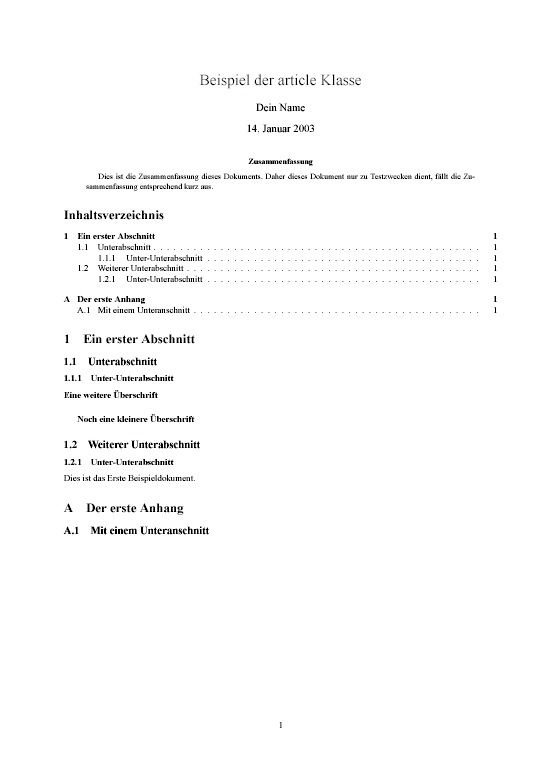
\includegraphics[height=5cm]{images/article_page1.png}}
	\end{center}
	\caption{Aufbau eines Dokuments mit \enquote{scrartcl}}
	\label{fig:article}
\end{figure}

\section{Dokumentklasse \enquote{scrreprt}}
\index{Dokumentklasse!scrreprt}

\begin{lstlisting}
\documentclass{scrreprt}
\end{lstlisting}

Ein \enquote{scrreprt} ist die gr��ere Form eines Dokuments. Das Dokument bekommt eine separate Titelseite, sowie eine separate Seite f�r die Zusammenfassung und das Inhaltsverzeichnis. Im Vergleich zu der Klasse \enquote{scrartcl} steht hier zudem das \enquote{Kapitel} mit dem Kommando \texttt{\textbackslash chapter} zur Verf�gung.

M�gliche Gliederungen in dieser Dokumentklasse sind somit:

\begin{itemize}
	\item \texttt{\textbackslash chapter}
	\item \texttt{\textbackslash section}
	\item \texttt{\textbackslash subsection}
	\item \texttt{\textbackslash subsubsection}
	\item \texttt{\textbackslash paragraph}
	\item \texttt{\textbackslash subparagraph}.
\end{itemize}

Das Beispiellisting \ref{lst:report} erzeugt sechs Seiten welche du auf Abbildung \ref{fig:report} siehst.

\begin{figure}[htb]
	\begin{center}
		\fbox{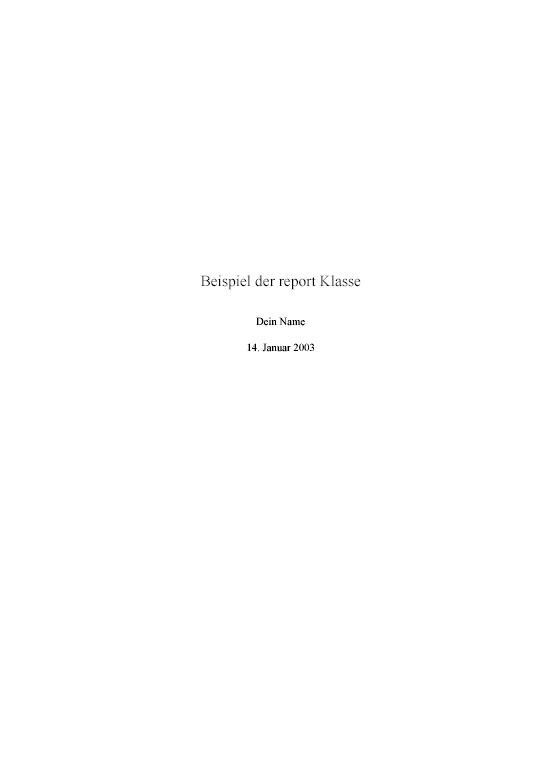
\includegraphics[height=5cm]{images/report_page1.png}}
		\fbox{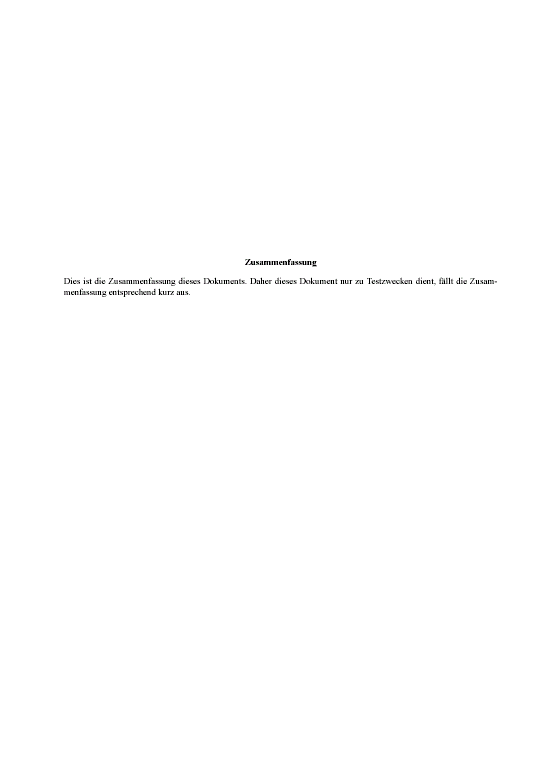
\includegraphics[height=5cm]{images/report_page2.png}}
		\fbox{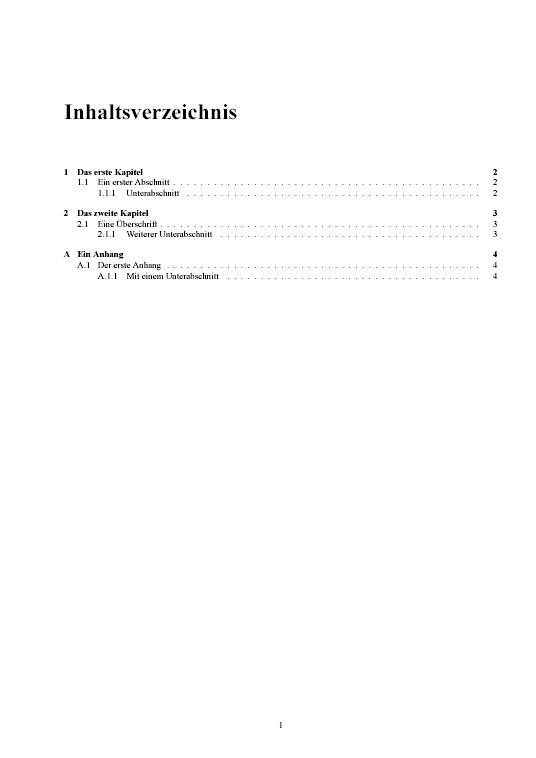
\includegraphics[height=5cm]{images/report_page3.png}} \\
		\fbox{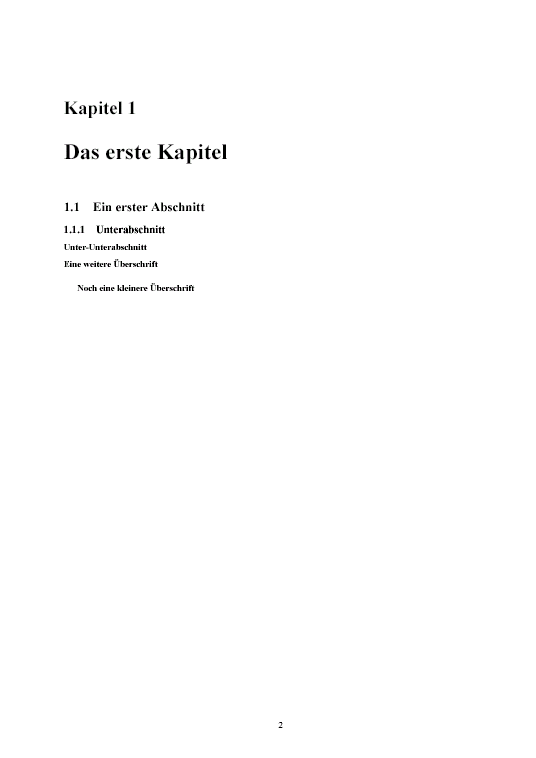
\includegraphics[height=5cm]{images/report_page4.png}}
		\fbox{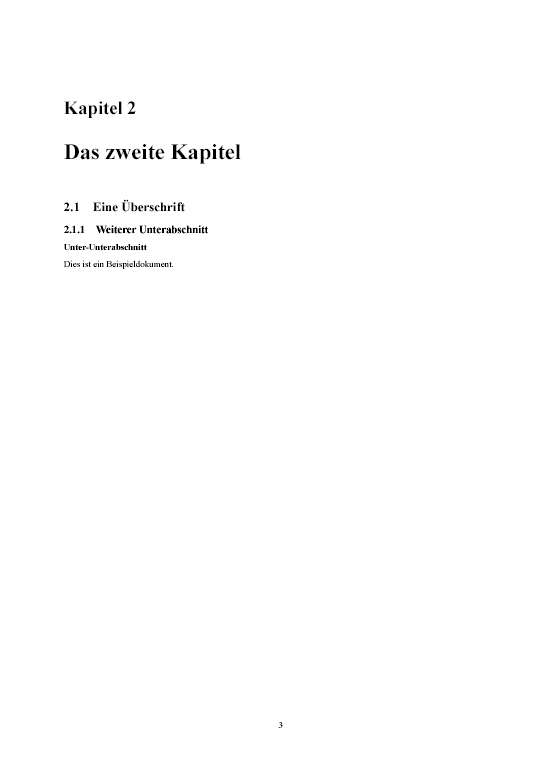
\includegraphics[height=5cm]{images/report_page5.png}}
		\fbox{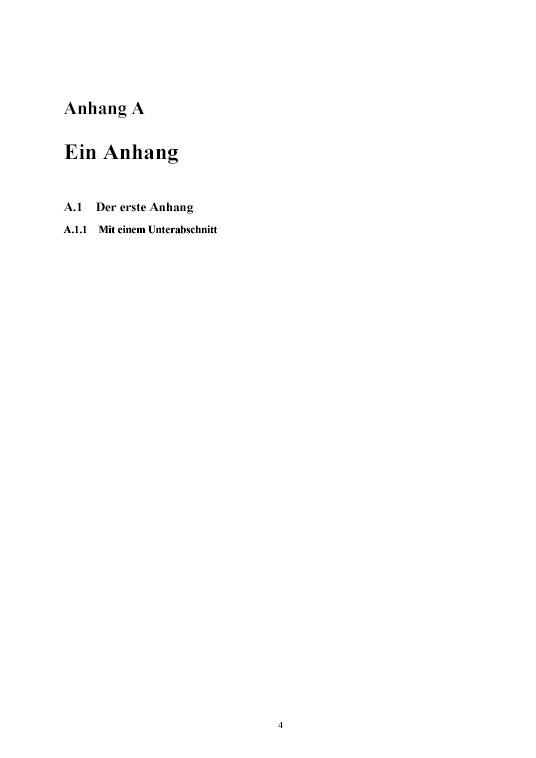
\includegraphics[height=5cm]{images/report_page6.png}}
	\end{center}
	\caption{Aufbau eines Dokuments mit \enquote{scrreprt}}
	\label{fig:report}
\end{figure}


\section{Dokumentklasse \enquote{scrbook}}
\index{Dokumentklasse!scrbook}

\begin{lstlisting}
\documentclass{scrbook}
\end{lstlisting}

Mit der Dokumentklasse \enquote{scrbook} werden die gr��ten Dokumente erstellt. Der Satz ist zweiseitig und die Kapitel beginnen immer auf einer rechten Seite. Nat�rlich ist der Titel und das Inhaltsverzeichnis auf einer eigenen Seite. In dieser Dokumentklasse existiert keine Zusammenfassung (abstract), da dies bei B�chern un�blich ist. 

Neu hinzu kommt der Befehl \texttt{\textbackslash part}, mit welchem du dein Buch in einzelne Teile unterteilen kannst.

M�gliche Gliederungen in dieser Dokumentklasse sind:
\begin{itemize}
	\item \texttt{\textbackslash part}
	\item \texttt{\textbackslash chapter}
	\item \texttt{\textbackslash section}
	\item \texttt{\textbackslash subsection}
	\item \texttt{\textbackslash subsubsection}
	\item \texttt{\textbackslash paragraph}
	\item \texttt{\textbackslash subparagraph}.
\end{itemize}

Das Beispiellisting \ref{lst:book} erzeugt neun Seiten, welche du auf Abbildung \ref{fig:book} siehst.

\begin{figure}[htb]
	\begin{center}
		\fbox{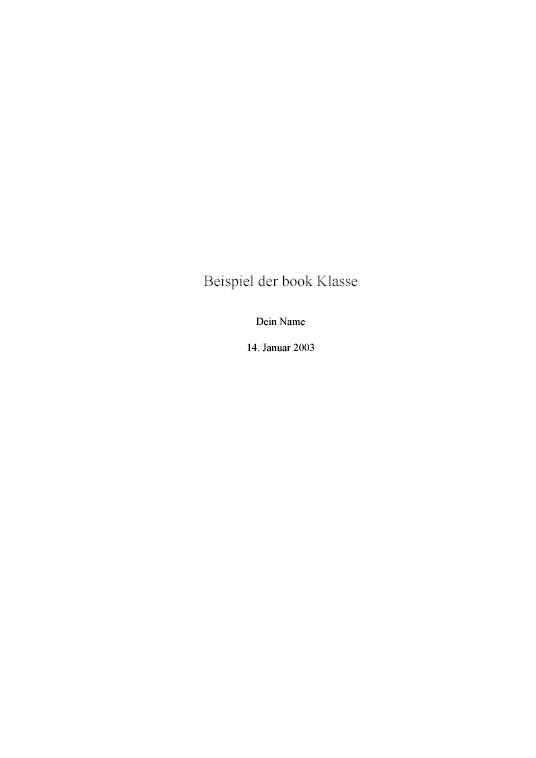
\includegraphics[height=5cm]{images/book_page1.png}}
		\fbox{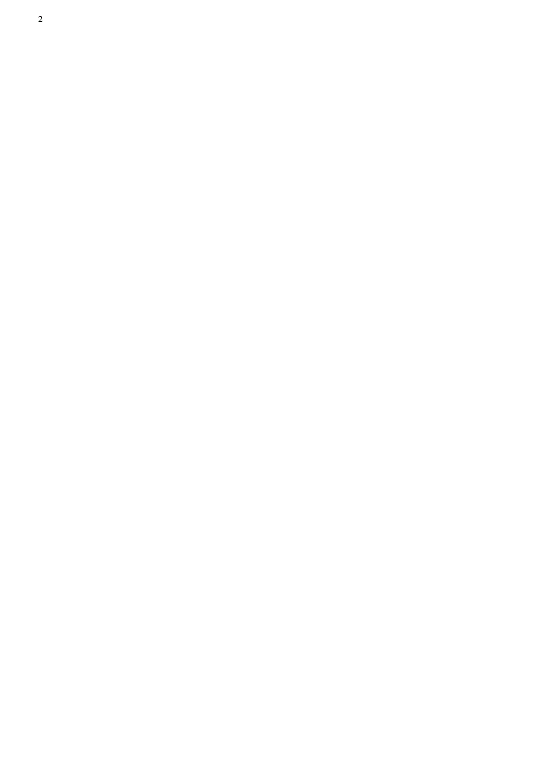
\includegraphics[height=5cm]{images/book_page2.png}}
		\fbox{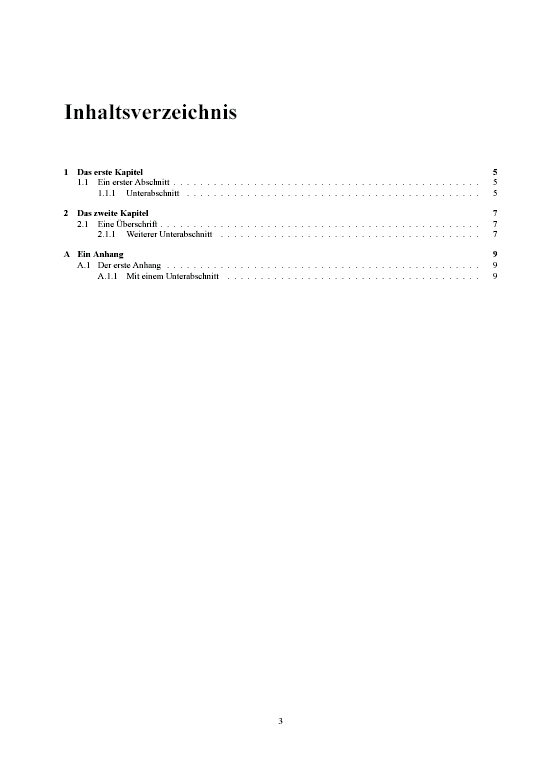
\includegraphics[height=5cm]{images/book_page3.png}} \\
		\fbox{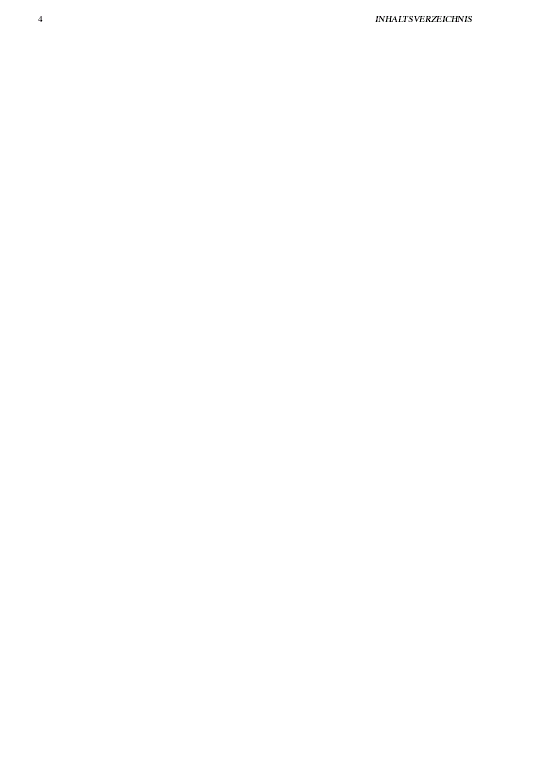
\includegraphics[height=5cm]{images/book_page4.png}}
		\fbox{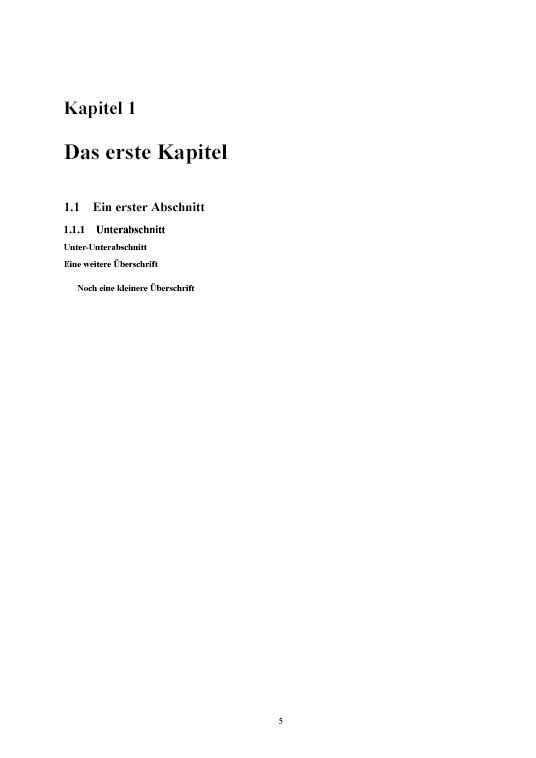
\includegraphics[height=5cm]{images/book_page5.png}}
		\fbox{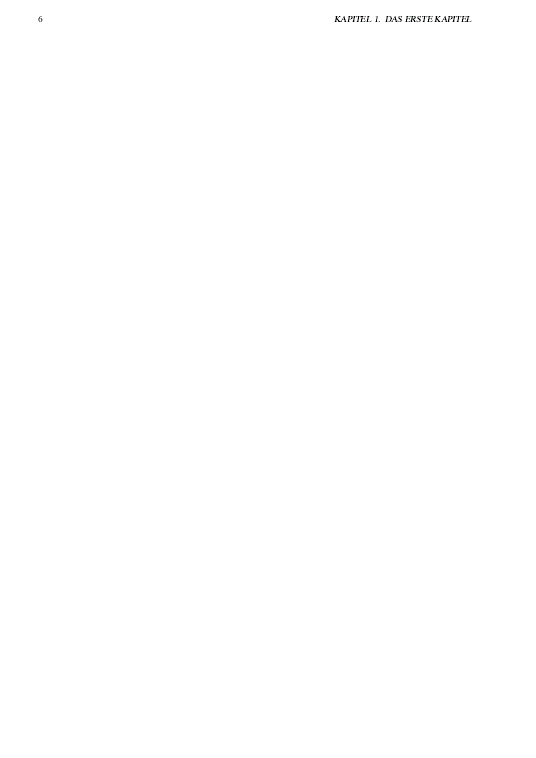
\includegraphics[height=5cm]{images/book_page6.png}} \\
		\fbox{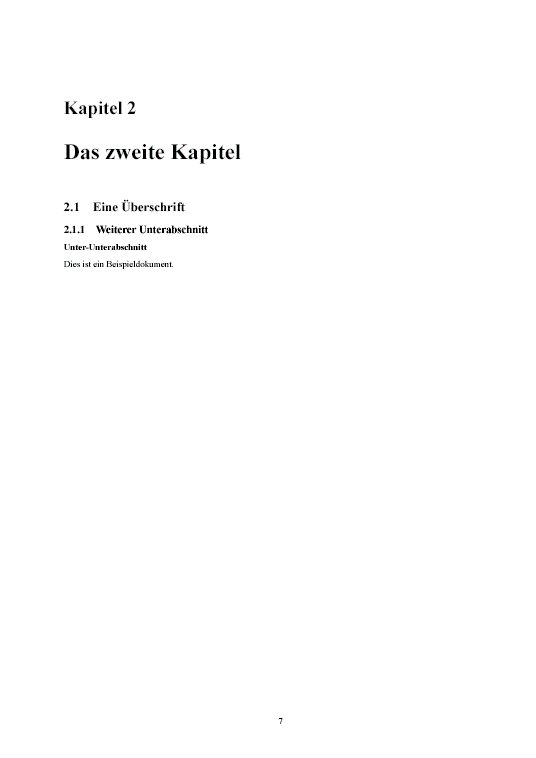
\includegraphics[height=5cm]{images/book_page7.png}}
		\fbox{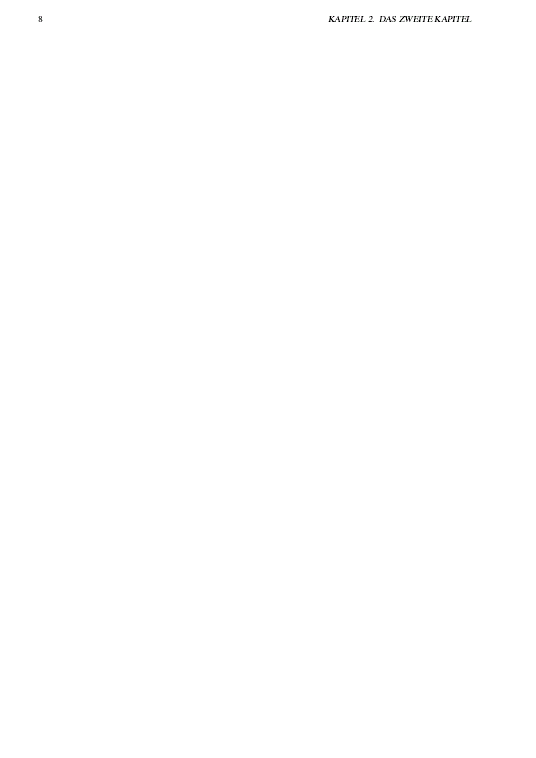
\includegraphics[height=5cm]{images/book_page8.png}}
		\fbox{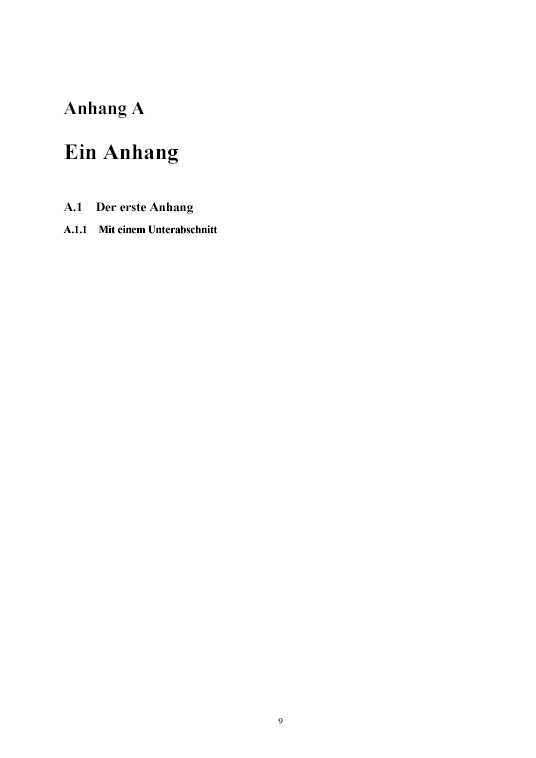
\includegraphics[height=5cm]{images/book_page9.png}}
	\end{center}
	\caption{Aufbau eines Dokuments mit \enquote{scrbook}}
	\label{fig:book}
\end{figure}

%
% EOF
%

%
% Diplomarbeit mit LaTeX
% ===========================================================================
% This is part of the book "Diplomarbeit mit LaTeX".
% Copyright (c) 2002-2005 Tobias Erbsland, Andreas Nitsch
% See the file diplomarbeit_mit_latex.tex for copying conditions.
%

\chapter{Tabellen und Bilder}
\label{sec:tabellenundbilder}

\section{Tabellen}
\index{Tabellen}

Tabellen sind in \DMLLaTeX \ ein Thema f�r sich. Ich beschreibe hier daher nur die sogenannte \enquote{tabular}\index{begin@\texttt{\textbackslash begin}!tabular} Umgebung. Um die tabular Umgebung nutzen zu k�nnen, solltest du zudem im Kopfbereich deines Dokuments das Paket \enquote{array}\index{Paket!array} einbinden. Das machst du mit dem Befehl:

\begin{lstlisting}
\usepackage{array}
\end{lstlisting}

Hier die erste Beispieltabelle:
\index{begin@\texttt{\textbackslash begin}!table}

\begin{lstlisting}
\begin{table}
	\centering
	\begin{tabular}{llr}
		\textbf{Farbe} & \textbf{Form} & \textbf{Zahl} \\
		Rot            & Rechteck      & 100 \\
		Blau           & Kreis         & 99 \\
		Gelb           & Dreieck       & 98 \\
	\end{tabular}
	\caption{Beispieltabelle 1}
	\label{tbl:beispieltabelle1}
\end{table}
\end{lstlisting}

Die einzelnen Spalten\index{Tabellen!Spalten} werden also mit dem \enquote{\texttt{\&}}-Zeichen getrennt und eine neue Tabellenzeile beginnt mit einem doppelten Backslash.

Direkt hinter dem Befehl \texttt{\textbackslash begin\{tabular\}} befindet sich der Parameter \texttt{\{llr\}}. Das bedeutet soviel wie: drei Spalten, die ersten beiden linksb�ndig formatiert, die letzte rechtsb�ndig. Je nach Buchstabe in diesem Parameter kann man die Spalten unterschiedlich formatieren. Einige Beispiele:

\begin{description}
	\item[\texttt{l}] Linksb�ndig formatierte Spalte.
	\item[\texttt{c}] Zentriert formatierte Spalte.
	\item[\texttt{r}] Rechtsb�ndig formatierte Spalte.
	\item[\texttt{p\{5cm\}}] Die Spalte ist genau 5cm breit.
	\item[\texttt{|}] F�gt hier eine vertikale Linie ein.
\end{description}

Das Beispiel oben siehst du als Tabelle \ref{tbl:beispieltabelle1}.

\begin{table}
	\centering
	\begin{tabular}{llr}
		\textbf{Farbe} & \textbf{Form} & \textbf{Zahl} \\
		Rot            & Rechteck      & 100 \\
		Blau           & Kreis         & 99 \\
		Gelb           & Dreieck       & 98 \\
	\end{tabular}
	\caption{Beispieltabelle 1}
	\label{tbl:beispieltabelle1}
\end{table}

\subsection{Linien in Tabellen}
\label{sec:linienintabellen}
\index{Linien in Tabellen}\index{Tabellen!Linien}

Es ist auch m�glich, Linien in der Tabelle einzubauen. F�r horizontale Linien verwendet man dabei den Befehl \texttt{\textbackslash hline}, f�r die vertikalen Linien macht man ein \enquote{\texttt{|}}-Zeichen zwischen die Spaltenangabe.

Solche \enquote{Kl�tzchentabellen} solltest du jedoch m�glichst vermeiden. Eine sehr gute Anleitung findest du unter~\cite{TabSatz}. Axel Reichert erkl�rt in diesem Dokument anhand von vielen Beispielen wie man Tabellen lesbar, eindeutig und �bersichtlich gestalten kann.

Das Beispiel mit einigen Linien:

\begin{lstlisting}
\begin{table}
	\centering
	\begin{tabular}{|l|l|r|}
		\textbf{Farbe} & \textbf{Form} & \textbf{Zahl} \\
		\hline
		Rot            & Rechteck      & 100 \\
		\hline
		Blau           & Kreis         & 99 \\
		\hline
		Gelb           & Dreieck       & 98 \\
		\hline
	\end{tabular}
	\caption{Beispieltabelle 2}
	\label{tbl:beispieltabelle2}
\end{table}
\end{lstlisting}

Das Beispiel siehst du als Tabelle \ref{tbl:beispieltabelle2}.

\begin{table}
	\centering
	\begin{tabular}{|l|l|r|}
		\textbf{Farbe} & \textbf{Form} & \textbf{Zahl} \\
		\hline
		Rot            & Rechteck      & 100 \\
		\hline
		Blau           & Kreis         & 99 \\
		\hline
		Gelb           & Dreieck       & 98 \\
		\hline
	\end{tabular}
	\caption{Beispieltabelle 2}
	\label{tbl:beispieltabelle2}
\end{table}

\subsection{Mehrere Spalten zusammenfassen}
\index{Tabellen!Spalten zusammenfassen}\index{Spalten zusammenfassen}

Falls du mehrere Spalten zusammenfassen m�chtest, kannst du das mit dem Befehl
\\
 \texttt{\textbackslash multicolumn} machen. Der Befehl hat drei Argumente: Die Anzahl der Spalten, welche zusammengefasst werden sollen, die Ausrichtung der Spalte und der Text, welcher in diesem Bereich angezeigt werden soll. Hier ein Beispiel:

\begin{lstlisting}
\begin{table}
	\begin{tabular}{|l|l|l|}
		\hline
		\multicolumn{2}{|c|}{\textbf{Form \& Farbe}} & \textbf{Zahl} \\
		\hline
		Rot            & Rechteck      & 100 \\
		\hline
		Blau           & \multicolumn{2}{|l|}{Doppelt} \\
		\hline
		\multicolumn{3}{|r|}{Noch eine Breite Spalte} \\
		\hline
	\end{tabular}
	\caption{Beispieltabelle 3}
	\label{tbl:beispieltabelle3}
\end{table}
\end{lstlisting}

Das Beispiel siehst du als Tabelle \ref{tbl:beispieltabelle3} auf Seite \pageref{tbl:beispieltabelle3}.

\begin{table}
	\centering
	\begin{tabular}{|l|l|l|}
		\hline
		\multicolumn{2}{|c|}{\textbf{Form \& Farbe}} & \textbf{Zahl} \\
		\hline
		Rot            & Rechteck      & 100 \\
		\hline
		Blau           & \multicolumn{2}{l|}{Doppelt} \\
		\hline
		\multicolumn{3}{|r|}{Noch eine Breite Spalte} \\
		\hline
	\end{tabular}
	\caption{Beispieltabelle 3}
	\label{tbl:beispieltabelle3}
\end{table}

\subsection{Tabellenbreite bestimmen bzw. automatischer Zeilenumbruch}
\index{Tabellen!Spaltenbeite bestimmen}\index{Tabellen!Automatischer Zeilenumbruch}

In konventionellen Tabellen werden lange Zeilen nicht automatisch umbrochen, sondern \DMLLaTeX \ schreibt froh und munter �ber den Seitenrand hinaus. Man kann manuelle Zeilenumbr�che mit \textbackslash \textbackslash \ einf�gen, was hart an Masochismus grenzt, wenn man mehr als eine Hand voll Tabellen hat und das Layout (R�nder, Schriftgr��e, \ldots) ge�ndert wird -- was bei gr��eren Arbeiten durchaus vorkommt, z.\,B. mal mit und mal ohne Korrekturrand, je nach Bindungsart unterschiedlicher Abstand usw.

\begin{table}[h]	
		\begin{tabular}{| l | l |}  
		  % man mu� alle Umbr�che manuell machen
			\hline
			Kurze				& Lange Spalteninhalte\\
			\hline
			Links kurz	&Und rechts absichtlich viel, viel zu langer Test-Text1, Test-Text2, Test-Text3, Test-Text4, Test-Text5, Test-Text6\\
			\hline			
		\end{tabular}
	\caption{Anschauungsbeispiel einer zu breit geratene Tabellenspalte}
	\label{tab:Tabelle_zu_breit}
\end{table}

\begin{table}[h]	
		\begin{tabular}{| l | l |}  
		  % man mu� alle Umbr�che manuell machen
			\hline
			Kurze				& Lange Spalteninhalte mit manuell eingef�gten Zeilenumbr�chen:\\
			\hline
			Links kurz	&Und rechts absichtlich viel, viel zu langer\\
									&Test-Text1, Test-Text2, Test-Text3, Test-Text4,\\
									&Test-Text5, Test-Text6\\
			\hline						
		\end{tabular}
	\caption{Eigentlich zu breite Tabellenspalte mit manuell eingef�gten Zeilenumbr�chen formatiert. Hat eine andere, aber sehr �hnliche Breite wie der Text, was nicht sonderlich h�bsch ist.}
	\label{tab:Tabelle_zu_breit_manuell}
\end{table}

Um die Zeilenumbr�che automatisiert setzen zu lassen, mu� man die Breite der Spalte(n) mit \enquote{zu viel} Text festlegen. Dabei k�nnen entweder absolute Werte verwendet werden, z.\,B. 5\,cm oder 10\,em, oder sog. \textit{command lengths}, sozusagen Variablen, deren Wert von der Dokumentenklasse und Pr�ambel abh�ngen, z.\,B. \textbackslash textwidth (Spaltenbreite in aktueller Umgebung). Ersteres ist exakter, aber man mu� bei jeder Layout�nderung \textit{alle} Tabellen �berpr�fen und ggf. alle Spaltenbreiten anpassen. L�stig. Letzteres ist grunds�tzlich angenehmer, kann aber im Einzelfall Probleme verursachen, z.\,B. wenn eine Spalte zu schmal f�r ein nicht trennbares Wort wird. Also Tabellen im Ausgabeformat genau anschauen. Nebenbei: Man kann in \DMLLaTeX \ rechnen, was wir Anschauungsbeispiel machen, indem wir \textbackslash textwidth mit 0.2 bzw. 0.74 multiplizieren.

\begin{table}[h]		
		\begin{tabular}{|p{0.2\textwidth} | p{0.74\textwidth} |}  
		  % automatisch an normale Textbreite angepa�t
			\hline
			Kurze				& Lange Spalteninhalte automatisch umbrochen\\
			\hline
			Links kurz	&Und rechts absichtlich viel, viel zu langer Test-Text1, Test-Text2, Test-Text3, Test-Text4, Test-Text5, Test-Text6\\
			\hline
		\end{tabular}
	\caption{Eigentlich zu breite Tabellenspalte automatisch umbrochen}
	\label{tab:Tabelle_zu_breit_automatisch}
\end{table}

Hier siehst Du den code der drei Arten von Tabellendefinitionen:

\begin{lstlisting}
\begin{table}[h]	
	\begin{tabular}{| l | l |} 
	  % man mu� alle Umbr�che manuell machen
	%\begin{tabular}{|p{0.25\textwidth} | p{0.75\textwidth} |} 
	  % automatisch an normale Textbreite angepa�t
	%\begin{tabular}{|p{3cm} | p{6cm}|} 
	  % man mu� ggf. alle Spaltenbreiten manuell anpassen	  
			\hline
			Kurze				& Lange Spalteninhalte\\
			\hline
			Links kurz	&Und rechts absichtlich viel, viel zu langer Test-Text1, Test-Text2, Test-Text3, Test-Text4, Test-Text5, Test-Text6\\
			\hline			
		\end{tabular}
	\caption{Absichtlich zu breit geratene Tabellenspalte}
	\label{tab:Tabelle_zu_breit}
\end{table}
\end{lstlisting}

Weitere \textit{command lengths} wie \textbackslash textwidth findest Du im Kochbuch \cite{Kochbuch}, Kapitel 8, Abschnitt L�ngen.

\section{Bilder}
\index{Bilder \see{Grafiken}}\index{Abbildungen \see{Grafiken}}\index{Grafiken}

In dein Dokument kannst du beliebige Bilder einbetten. Dabei kannst du alle Bildformate\index{Grafiken!Format} verwenden, welche in einer PDF-Datei zul�ssig sind. Dies sind die Formate GIF, PNG und JPEG.

Wenn du jedoch ein DVI- oder eine PostScript-Datei erzeugen m�chtest, dann sind nur PostScript- oder Embedded-PostScript-Dateien zul�ssig.

Das GIF-Format solltest du nicht verwenden, da dies rechtliche Konsequenzen mit sich bringt. Lies dazu den Kommentar unter~\cite{NoGIF}.
%TODO: Das entsprechende Patent ist 2004 ausgelaufen. Meines Wissens kann gif nun bedenkenlos
%verwendet werden.

Um Grafiken in dein Dokument einzubetten, solltest du das Paket \enquote{graphicx}\index{Paket!graphicx} im Kopfbereich deines Dokuments einbinden. Dies machst du mit folgendem Befehl:

\begin{lstlisting}
\usepackage{graphicx}
\end{lstlisting}

Jetzt kannst du mit dem Befehl \texttt{\textbackslash includegraphics}\index{includegraphics@\texttt{\textbackslash includegraphics}} Grafiken in dein Dokument einbetten:

\begin{lstlisting}
\includegraphics{images/apfel.png}
\end{lstlisting}

Dabei gibt \enquote{images/apfel.png} den Pfad relativ zu deinem Dokument und den Dateinamen des Bildes an, welches du einf�gen m�chtest.

Am Besten legst du in deinem Dokumentverzeichnis ein Unterverzeichnis \enquote{images} an. Dann kopierst alle Bilder, welche du in deinem Dokument verwendest, in dieses Verzeichnis. So ist es einfacher, den �berblick in der Verzeichnisstruktur zu behalten. Sprechende Namen bei den Bilddateien sind sicher auch sehr hilfreich.

\subsection{Einf�gen einer Grafik in einem Float}
\index{Grafiken!Float}\index{begin@\texttt{\textbackslash begin}!figure}

Dies f�gt eine Grafik genau an der Stelle in einem Text ein, an der der Befehl hierzu steht. Normalerweise f�gt man Grafiken jedoch auch in einer speziellen Umgebung in den Text ein, so dass man die Grafik mit einem Titel versehen und Referenzen darauf setzen kann. Deshalb hier eine sogenannte Float-Umgebung, welche die Grafik in das Dokument einbettet, in der Mitte der Seite zentriert, ein Label\index{Grafiken!Label}\index{Grafiken!Beschriftung} definiert und beschriftet:

\begin{lstlisting}
\begin{figure}[htb]
	\centering
	\includegraphics{images/apfel.png}
	\caption{Ein Apfel}
	\label{fig:apfel}
\end{figure}
\end{lstlisting}

\subsection{Skalieren von Grafiken}
\index{Grafik!skalieren}

Der Befehl \texttt{\textbackslash includegraphics} kennt noch mehr Parameter als den Dateinamen des einzubettenden Bildes: Einer der h�ufig gebrauchten ist der \enquote{width} Parameter. Dieser skaliert die Grafik auf die angegebene Breite. Im folgenden Beispiel wird die Grafik auf 5cm Breite skaliert:

\begin{lstlisting}
\includegraphics[width=5cm]{images/apfel.png}
\end{lstlisting}

Dieses Beispiel skaliert die Grafik genau auf die Textbreite: \index{Grafiken!Textbreite}

\begin{lstlisting}
\includegraphics[width=\textwidth]{images/apfel.png}
\end{lstlisting}

Und noch ein letztes Beispiel, welches die Grafik auf 50\% der Textbreite skaliert:

\begin{lstlisting}
\includegraphics[width=0.50\textwidth]{images/apfel.png}
\end{lstlisting}

Weiter ist es m�glich, die Grafik zuzuschneiden und zu rotieren. Diese und weitere Optionen findest du in der Dokumentation zum \enquote{graphicx} Paket. Die Dokumentation befindet sich im \enquote{doc} Verzeichnis deiner MiKTeX Installation.




\section{Floats}
\index{Floats}

Sowohl bei den Tabellen wie auch bei den Grafiken (Abbildungen) verwendest du eine sogenannte \enquote{float}-Umgebung, um die Tabelle oder die Abbildung in den Text einzubetten.

Dabei entscheidet \DMLLaTeX \ selbst�ndig, wo genau die Abbildung im endg�ltigen Dokument erscheint. Um innerhalb deines Textes auf die Tabelle oder die Abbildung zu verweisen, verwendest du Referenzen.

An welcher Stelle ein Float platziert werden kann, kannst du mit optionalen Argumenten bei der Float-Umgebung steuern. Diese Argumente sind jedoch h�chstens Vorschl�ge, keine Anweisungen. Hier ein Beispiel:

\begin{lstlisting}
Gerade im Herbst ist die Erntezeit der �pfel. Ein Apfel siehst du 
auf Abbildung \ref{fig:apfel} auf Seite \pageref{fig:apfel}.

\begin{figure}[hb]
	\centering
	\includegraphics{images/apfel.png}
	\caption{Ein Apfel}
	\label{fig:apfel}
\end{figure}
\end{lstlisting}

In Zeile 4 dieses Beispiels siehst du hinten an dem Befehl \texttt{\textbackslash begin\{figure\}} den optionalen Parameter \texttt{\[hb.\]} Das besagt soviel wie: bette diese Grafik m�glichst hier (h) oder unten an der Seite (b) ein. Die m�glichen Buchstaben sind:

\begin{description}
\item[h] Here. M�glichst an der Stelle, an der du den Float im Text eingebettet hast.
\item[t] Top. Oben an der Seite.
\item[b] Bottom. Unten an der Seite.
\item[p] Page. Auf einer separaten Seite.
\end{description}

In Zeile 9 wird ein Label \enquote{fig:apfel} definiert. Dadurch kannst du an einer beliebigen Stelle in deinem Dokument auf deine Tabelle oder Abbildung verweisen. Jede als Float eingef�gte Abbildung wird fortlaufend nummeriert. Mit dem Befehl \texttt{\textbackslash ref} kannst du auf die eingef�gte Abbildung bzw. Abbildungsnummer verweisen, mit dem Befehl \texttt{\textbackslash pageref} auf die Seite, auf der die Abbildung eingef�gt wurde.









%
% Diplomarbeit mit LaTeX
% ===========================================================================
% This is part of the book "Diplomarbeit mit LaTeX".
% Copyright (c) 2002-2008 Tobias Erbsland, Andreas Nitsch
% See the file diplomarbeit_mit_latex.tex for copying conditions.
%

\chapter{Dokumentteile}
\index{Dokumentteile|(}

Ein Dokument besteht normalerweise aus einzelnen, in sich geschlossenen Dokumentteilen:

\begin{itemize}
	\item Titelseite
	\item Inhaltsverzeichnis
	\item Inhalt
	\item Anhang
\end{itemize}

Diese einzelnen Teile kannst du mit \DMLLaTeX{} einfach einfügen, bzw. aufbauen.

\section{Anpassen der Titelseite}
\index{Titelseite}\index{Anpassen!Titelseite}

Um eine Titelseite aufzubauen, hast du mehrere Möglichkeiten. Im Kapitel \ref{sec:grundlagen} wird der einfachste Weg mit dem Kommando \texttt{\textbackslash maketitle} aufgezeigt.

Dabei setzt man im Header oder zumindest vor dem Befehl die notwendigen Angaben:
\begin{lstlisting}
\title{Diplomarbeit}
\author{Hans Muster}
\date{2005-12-12} % optional

\maketitle
\end{lstlisting}

Das Argument \texttt{\textbackslash date} ist dabei optional. Wenn du es weglässt, wird automatisch das aktuelle Datum eingefügt. 

In einem Artikel (\enquote{article}) wird der Titel einfach oben an das aktuelle Dokument mit einer großen Schriftart gesetzt. Das Dokument oder Inhaltsverzeichnis beginnt direkt darunter. In einem Buch (\enquote{book}) entsteht so eine separate Titelseite.

\subsection{Separate Titelseite in einem Artikel}
\label{sec:separatetitelseite}
\index{Separate Titelseite}

Falls du in einem Artikel eine separate Titelseite wünschst, kannst du das über die Klassenoption \enquote{titlepage} erreichen. Wie man eine solche Klassenoption setzt, kannst du in Kapitel \ref{sec:globaleoptionen} nachlesen.

\subsection{Eine eigene Titelseite erstellen}
\index{Eigene Titelseite}

Die Umgebung \enquote{titlepage} eignet sich vor allem dafür, wenn du eine eigene Titelseite erstellen möchtest. Dabei musst du jedoch einige der unterliegenden {\rmfamily\TeX} Kommandos kennen, welche die Grundlage von \DMLLaTeX{} bilden.

Hier als Beispiel die Titelseite dieses Dokuments:
\begin{lstlisting}[frame=tb, caption=Titelseite dieses Dokuments]
\begin{titlepage}
	\vspace*{7cm}
	\begin{center}
		\Huge
		Diplomarbeit mit \DMLLaTeX\\
		\vspace{1cm}
		\large
		Version 1.2\\
		\vspace{2cm}
		Tobias Erbsland <te@profzone.ch>\\
		Andreas Nitsch\\
	\end{center}
	\normalsize
	\vfill
	Copyright (c) 2002, 2003, 2005  Tobias Erbsland.

	Permission is granted to copy, distribute and/or modify this document
	under the terms of the GNU Free Documentation License, Version 1.2
	or any later version published by the Free Software Foundation;
	with no Invariant Sections, no Front-Cover Texts, and no Back-Cover Texts.
	A copy of the license is included in the section entitled \enquote{GNU
	Free Documentation License}.
\end{titlepage}
\end{lstlisting}

\section{Verzeichnisse}
\index{Verzeichnisse|(}

Inhaltsverzeichnisse werden in \DMLLaTeX{} automatisch erzeugt. Es ist möglich ein Inhaltsverzeichnis, ein Abbildungsverzeichnis und ein Tabellenverzeichnis ohne großen Aufwand in das Dokument einzubetten.

\DMLLaTeX{} geht dabei folgendermaßen vor: beim ersten Durchlauf werden die Seitennummern und Titel aller relevanten Überschriften und Beschriftungen in einer separaten Datei gespeichert (.aux). Aus dieser Datei werden am Schluss einzelne Dateien mit den verschiedenen Inhaltsverzeichnissen erstellt (.toc, .lot, .lof).

Beim nächsten Durchlauf werden diese Dateien für das Inhaltsverzeichnis und die anderen Verzeichnisse verwendet. Da sich die Seitennummerierung dadurch verändern kann (weil z.\,B. das Inhaltsverzeichnis um fünf Zeilen wächst), wird evtl. ein weiterer Durchlauf notwendig.

Die Seitenverweise sind daher frühestens nach dem zweiten oder sogar dritten Durchlauf des Dokuments korrekt. Bevor du also die endgültige Fassung deines Dokuments erstellst, solltest du das Dokument sooft kompilieren, bis keine Warnungen wie die folgende mehr auftreten:
\begin{lstlisting}
LaTeX Warning: Label(s) may have changed. Rerun to get cross-references right.
\end{lstlisting}

\subsection{Inhaltsverzeichnis}
\index{Inhaltsverzeichnis}

Das Inhaltsverzeichnis wird aus den Überschriften des Dokuments gebildet. Du kannst es mit folgendem Befehl in dein Dokument einbetten:
\begin{lstlisting}
\tableofcontents
\end{lstlisting}

Falls du möchtest, dass ein bestimmter Abschnitt nicht im Inhaltsverzeichnis auftaucht, kannst du die \enquote{*}-Schreibweise verwenden:
\begin{lstlisting}
\subsection*{Nicht im Inhaltsverzeichnis}
\end{lstlisting}

Möglicherweise ist der Titel im Dokument zu lang für das Inhaltsverzeichnis. Du hast daher die Möglichkeit den Eintrag, welcher im Inhaltsverzeichnis gemacht wird, vom Titel im Dokument zu trennen:
\begin{lstlisting}
\subsection[Kurzer Titel im Inhaltsverz.]{Hier der Lange
	Titel, welcher leider im Inhaltsverzeichnis keinen Platz gefunden
	hat.}
\end{lstlisting}
 

\subsection{Abbildungsverzeichnis und Tabellenverzeichnis}
\index{Abbildungsverzeichnis}\index{Tabellenverzeichnis}

Das Abbildungsverzeichnis und das Tabellenverzeichnis werden aus den \texttt{\textbackslash caption} Einträgen innerhalb der \enquote{figure} und \enquote{table} Floats gebildet. 

Die beiden Verzeichnisse kannst du folgendermaßen in dein Dokument einbetten:
\begin{lstlisting}
\listoffigures
\listoftables
\end{lstlisting}

\index{Verzeichnisse|)}

\section{Anhang}
\index{Anhang}

Oft hat ein Dokument noch Anhänge. Das sind Kapitel oder Anschnitte, welche zusätzliche Informationen zu dem Thema des Dokuments erhalten, z.\,B. Tabellen, Diagramme oder große Grafiken, welche oft aus dem Dokument referenziert werden, jedoch nicht in ein bestimmtes Kapitel des Dokuments passen. Ein Beispiel hierfür ist die API-Referenz einer Software.

Der Anhang wird mit dem Befehl \texttt{\textbackslash appendix}\index{appendix@\texttt{\textbackslash appendix}} eingeleitet. Nach diesem Befehl werden die Kapitel oder Abschnitte mit Großbuchstaben nummeriert.
\begin{lstlisting}[frame=tb, caption=Dokumentstruktur mit Anhang]
\section{Dokumentinhalt}
\subsection{Untertitel des Dokumentinhalts}

\section{Weiterer Dokumentinhalt}

\appendix % Ab hier beginnt der Anhang

\section{Erster Anhang}
\subsection{Untertitel des ersten Anhangs}

\section{Zweiter Anhang}

\end{lstlisting}

\index{Dokumentteile|)}


%
% Diplomarbeit mit LaTeX
% ===========================================================================
% This is part of the book "Diplomarbeit mit LaTeX".
% Copyright (c) 2002-2005 Tobias Erbsland, Andreas Nitsch
% See the file diplomarbeit_mit_latex.tex for copying conditions.
%
\chapter{Mathematischer Textsatz}
\index{Formeln}\index{Mathematik}

In \DMLLaTeX \ ist eine sehr mächtige Mathematik-Umgebung integriert, mit welcher du nahezu beliebige mathematische Formeln setzen kannst. Hier ein Beispiel einer sinnlosen, komplizierten Formel
\begin{equation}
	x = 12 \cdot \left( \frac{
		\sqrt[g]{ \frac{ 100 + \chi }{ \cos 45^{f} } }
	}{
		\lfloor \frac{ t - \beta }{ \sqrt{ r } } \rfloor
		+ \left( \frac uv \right)^2
	} \right) + \lVert a\rVert - \int_\Omega \sin(\tau) d\tau,
\end{equation}
an dem du erahnen kannst, was möglich ist.

Da das Setzen mathematischer Formeln ein Thema ist, welches allein mehrere Bücher füllen kann, möchte ich dir in diesem Kapitel nur einige wichtige Kommandos zeigen. Weitere Informationen findest du also in Büchern oder im Internet. Neben einigen Manuals, die im Folgenden genannt sind, ist als Nachschlagewerk die umfangreiche und mit Beispielen ausgestattete \TeX-Hilfe der Wikipedia\footnote{\href{https://de.wikipedia.org/wiki/Hilfe:TeX}{https://de.wikipedia.org/wiki/Hilfe:TeX}} zu empfehlen. Sie ist zwar eigentlich für den wikipedia-internen Formelsatz gedacht, aber in den meisten Fällen auch fürs konventionelle \TeX{}en sehr hilfreich.

Einige wichtige Symbole und Konstrukte kannst du über das Menü \enquote{Mathe} von TeXnicCenter direkt in deinen Quelltext einfügen. Jedoch hinkt dieses Menü den modernen mathematischen Packages teilweise hinterher, weshalb es geschickter ist, sich die neuesten Manuals aus dem Internet herunterzuladen und zu studieren.

Wenn du komplexere Formeln in deinem Dokument verwendest oder viele mathematische Formeln benötigst, solltest du die Pakete der American Mathematical Society (kurz: \AmS) einbinden und deren relativ kurzgehaltene Manuals lesen. Die \AmSmath-Packages stellen weitere Symbole und spezielle mathematische Umgebungen bereit. Eine detaillierte Erklärung zu den Packages bietet die \AmS\ auf ihrer Website sowie das CTAN.\footnote{Der URL des {\rmfamily\LaTeX}-Teils der Website der \AmS\ lautet \href{https://www.ams.org/tex/amslatex.html}{https://www.ams.org/tex/amslatex.html}; im CTAN, genauer auf \href{https://www.ctan.org/pkg/amslatex}{https://www.ctan.org/pkg/amslatex} sind ebenfalls kurze Infos zu den einzelnen Packages abrufbar.} Eingebunden werden die Packages beispielsweise durch

\begin{lstlisting}
\usepackage{amsmath, amsthm, amssymb}
\usepackage{mathtools}
\end{lstlisting}

Empfehlenswert ist das im Beispiel zuletzt genannte Package \enquote{mathtools}, eine sehr nützliche Erweiterung der \AmSmath-Packages.\footnote{\href{https://www.ctan.org/pkg/mathtools}{https://www.ctan.org/pkg/mathtools}}

Wer sich intensiv mit mathematischen Formeln rumschlagen will, dem wird das Dokument Mathmode\footnote{\href{https://www.ctan.org/pkg/voss-mathmode}{https://www.ctan.org/pkg/voss-mathmode}} sehr hilfreich sein. Es geht auf viele Feinheiten ein, die z.\,B. in den \AmSmath-Manuals nicht oder nur sehr kurz abgehandelt werden.

Mit diesen Packages sollte man auch für mathematische Abschlussarbeiten -- zumindest bzgl. des Formelsatzes -- gerüstet sein.

\section{Die Gleichungsumgebungen}
\subsection{Einbettung in Text}

Eine kurze mathematische Formel innerhalb von Fließtext schließt du einfach in zwei Dollarzeichen (\$) ein, also z.\,B.

\begin{lstlisting}
$100 + a^2$
\end{lstlisting}

Damit bettest du die mathematische Formel oder auch nur ein einzelnes Zeichen in den Text ein. Die Formel aus dem Beispiel sieht z.\,B. so aus: $100 + a^2$. Du siehst, dass zum Setzen der Formel ein spezieller Zeichensatz verwendet wird. Dadurch kann sehr gut zwischen normalem Text und mathematischen Formeln unterschieden werden.

\begin{lstlisting}
\begin{quote}
	Die Hypothenuse $c$ eines rechtwinkligen Dreiecks kann mit der Formel 
	des Pythagoras ermittelt werden. Dabei müssen die Katheten $a$ und $b$
	des Dreiecks bekannt sein. Die Formel lautet: $c = \sqrt{a^2 + b^2}$. 
\end{quote}
\end{lstlisting}

Dies sieht dann im Text folgendermaßen aus:

\begin{quote}
	Die Hypothenuse $c$ eines rechtwinkligen Dreiecks kann mit der Formel 
	des Pythagoras ermittelt werden. Dabei müssen die Katheten $a$ und $b$
	des Dreiecks bekannt sein.
	Die Formel lautet: $c = \sqrt{a^2 + b^2}$. 
\end{quote}

\subsection{Einfache abgesetzte Formeln}

Abgesetzte Formeln innerhalb deines Dokuments kannst du z.\,B. mithilfe der \enquote{equation}-Umgebung einbauen:

\begin{lstlisting}
\begin{equation}
	c = \sqrt{a^2 + b^2}
\end{equation}
\end{lstlisting}

Im Gegensatz zum Einbetten in den Quelltext mit dem Dollarzeichen wird in dieser Umgebung die Formel nicht auf eine Zeilenhöhe gestaucht. Sie wird z.\,B.
\begin{equation}
	c = \sqrt{a^2 + b^2}
\end{equation}
gesetzt.

\subsection{Umgebungen für mehrere Gleichungen}

Neben den Umgebungen für eine einzelne Formel existieren weitere Umgebungen, mit denen du mehrere Formeln mit sehr unterschiedlichen Anordnungen setzen kannst. Die \AmSmath-Pakete liefern hierfür u.\,a. die Umgebungen \enquote{align}, \enquote{gather}, \enquote{split}, \enquote{multline}, \enquote{flalign} und \enquote{alignat}. Bis auf \enquote{split} lässt sich bei allen genannten Umgebungen die automatische Nummerierung durch einen nachgestellten Stern \enquote{*} deaktivieren. Die häufig von Laien verwendete Umgebung \enquote{eqnarray} ist nicht voll kompatibel zu den \AmSmath-Paketen und deshalb zu vermeiden\footnote{Nähere infos dazu stehen im \DMLLaTeX-Sündenregister\\\href{ftp://ftp.dante.de/tex-archive/info/l2tabu/german/l2tabu.pdf}{ftp://ftp.dante.de/tex-archive/info/l2tabu/german/l2tabu.pdf}} und z.\,B. durch \enquote{align} zu ersetzen. Damit kannst du z.\,B. Formeln an den Gleichheitszeichen ausrichten.

Der Code

\begin{lstlisting}
\begin{equation}
	a + a = 2a
\end{equation}

\begin{align}
	    a + a &= 2a \\
	a^2 + a^2 &= 2a^2 \\
	    a - a &= 0
\end{align}
\end{lstlisting} 

wird umgesetzt zu

\begin{equation}
	a + a = 2a
\end{equation}

\begin{align}
	    a + a &= 2a \\
	a^2 + a^2 &= 2a^2 \\
	    a - a &= 0.
\end{align}

Du kannst die Form \texttt{\textbackslash begin\{align*\}} verwenden, wenn du keine Nummerierung der Formeln wünschst. Einzelne Nummern kannst du mit dem Befehl \texttt{\textbackslash nonumber} direkt vor dem \texttt{\textbackslash \textbackslash } unterdrücken.

\section{Hoch- und tiefgestellte Ausdrücke}

Einzelne Zeichen kannst du direkt mit einem Zirkumflex (\texttt{\^}) oder einem Unterstrich (\texttt{\_}) hoch- bzw. tiefstellen. Um mehrere Zeichen oder komplexe Ausdrücke hoch- oder tiefzustellen, musst du jene in geschweifte Klammern \texttt{\{\}} %ohne umgebende () ist {} besser lesbar
einschließen.

%durch fortlaufende Nummern + Buchstaben (statt wiederkehrend dieselben) wird es für Leser leichter, die einzelnen Bsp voneinander zu trennen [anmerkung von seth: das halt' ich fuer'n geruecht. abgesehen davon, soll hier imho gar nix getrennt werden, ist doch immer dasselbe...]

Im beispielhaften Code
\begin{lstlisting}
\begin{equation}
	a^2 - b_1
	\qquad
	b_1^2 + b_2^2 
	\qquad
	c^{20} + c^{d + e} 
	\qquad
	f_{40}
	\qquad
	(g + h)_{50}
	\qquad
	i^12_k
	\qquad
	\sum^m_{i=1} \frac 1i
\end{equation}
\end{lstlisting} 
wird das Kommando \texttt{\textbackslash qquad} dazu verwendet, einen ausreichenden Abstand zwischen den einzelnen Ausdrücken einzufügen. Gesetzt ergibt das Ganze dann

\begin{equation}
	a^2 - b_1
	\qquad
	b_1^2 + b_2^2 
	\qquad
	c^{20} + c^{d + e} 
	\qquad
	f_{40}
	\qquad
	(g + h)_{50}
	\qquad
	i^12_k
	\qquad
	\sum^m_{i=1} \frac 1i.
\end{equation}

\section{Normaler Text in Formeln}

Oft möchte man \enquote{sprechende} Formeln verwenden, welche aus normalen Text bestehen, aber trotzdem von den mathematischen Konstrukten profitieren. Dies geht mit dem Befehl \texttt{\textbackslash text}, mit dem man normalen Text in eine Formel einbetten kann.

Der Beispiel-Code

\begin{lstlisting}
\begin{equation}
	\text{Leistung} = \frac{ \text{Arbeit} }{ \text{Zeit} }
\end{equation}
\end{lstlisting} 

ergibt die aus der Physik bekannte Formel

\begin{equation}
	\text{Leistung} = \frac{ \text{Arbeit} }{ \text{Zeit} }.
\end{equation}

Um Gleichungsumformungen zu kommentieren, ohne jedoch die einheitliche Ausrichtung am Gleichheitszeichen zu gefährden, bietet sich \enquote{intertext} an.

Durch

\begin{lstlisting}
\begin{quote}
	\begin{align}
		F &= f_1 + f_2 + f_3 + f_4 + f_5 + f_6 + f_7 + f_8 + \dotsb + f_{20}\\
		\intertext{lässt sich mittels des Summenoperators offensichtlich zu}
		F &= \sum_{i=1}^{20}f_i.\\
	\end{align}
	verkürzen.
\end{quote}
\end{lstlisting}

werden die Zeilen
\begin{quote}
	\begin{align}
		F &= f_1 + f_2 + f_3 + f_4 + f_5 + f_6 + f_7 + f_8 + \dotsb + f_{20}\\
		\intertext{lässt sich mittels des Summenoperators offensichtlich zu}
		F &= \sum_{i=1}^{20}f_i.
	\end{align}
	verkürzen.
\end{quote}
generiert.

\section{Brüche und Wurzeln}

Die Brüche und Wurzeln passen sich in der Größe automatisch an die Formel an, welche sie umschließen.

Die Beispiele

\begin{lstlisting}
\begin{equation}
	\frac ab
	\qquad
	\frac{\frac ab}{\frac cd}
	\qquad
	\sqrt a
	\qquad
	\sqrt{ \frac{a + b}{c - d} }
	\qquad
	\sqrt[b]{a}
\end{equation}
\end{lstlisting} 

sehen dann so

\begin{equation}
	\frac ab
	\qquad
	\frac{\frac ab}{\frac cd}
	\qquad
	\sqrt a
	\qquad
	\sqrt{ \frac{a + b}{c - d} }
	\qquad
	\sqrt[b]{a}
\end{equation}

aus.

\section{Funktionen}

Für die am häufigsten verwendeten Funktionen existieren entsprechende Befehle, welche die Namen dieser Funktionen passend in die Formel einfügen.

\begin{lstlisting}
\begin{equation}
	\arccos(x)
	\qquad
	\sin(x)
	\qquad
	\lg 12
\end{equation}
\end{lstlisting} 

Ausgespuckt wird hiermit

\begin{equation}
	\arccos(x)
	\qquad
	\sin(x)
	\qquad
	\lg 12.
\end{equation}

Es können jedoch im Header auch eigene Operatoren definiert, z.\,B.
\begin{lstlisting}
\DeclareMathOperator{\rg}{Rang}
\DeclareMathOperator{\dom}{dom}
\DeclareMathOperator{\diag}{diag}
...
\begin{document}
...
$\diag C, \rg(A-\lambda I), \dom M$
\end{lstlisting}

\section{Begrenzungssymbole (Klammern)}

Begrenzungssymbole, z.\,B. Klammern, schließen einen Formelausdruck ein.\\
Wenn du die normalen Klammen verwendest, passen sich diese nicht in der Höhe an die Formel an. Dazu gibt es spezielle Ausdrücke, welche du in

\begin{lstlisting}
\begin{gather*}
	(x)
	\qquad
	(\frac xy)
	\qquad
	\left(x\right)
	\qquad
	\left(\frac xy\right)
	\qquad
	\left\lvert \frac xy \right\rvert\\
	i\in\left\{1,\dotsc,\binom n k\right\}
\end{gather*}
\end{lstlisting} 

siehst. Naja, eigentlich siehst du erst in der Übersetzung

\begin{gather*}
	(x)
	\qquad
	(\frac xy)
	\qquad
	\left(x\right)
	\qquad
	\left(\frac xy\right)
	\qquad
	\left\lvert \frac xy \right\rvert\\
	i\in\left\{1,\dotsc,\binom n k\right\}
\end{gather*}
deren Wirkung. An den letzten Beispielen wird zudem deutlich, dass dieser Automatismus nicht nur auf die gewöhnlichen runden Klammern beschränkt ist.

Durch \verb|\left| und \verb|\right| wird die Größe der Klammern verändert, wobei sich Größe an der minimalen und maximalen Höhe des eingeschlossenen Ausdrucks orientiert. Manchmal führt dieser Automatismus zu unhübschen Ergebnissen, weshalb es auch möglich ist, die Größe manuell zu beeinflussen.

\begin{lstlisting}
\begin{gather*}
	\Biggl( \biggl( \Bigl( \bigl( (x) \bigr) \Bigr) \biggr) \Biggr)\\
	f(x(a-b))\\
	f\left(x(a-b)\right)\\
	f\bigl(x(a-b)\bigr)
\end{gather*}
\end{lstlisting} 

Übersetzt:
\begin{gather*}
	\Biggl( \biggl( \Bigl( \bigl( (x) \bigr) \Bigr) \biggr) \Biggr)\\
	f(x(a-b))\\
	f\left(x(a-b)\right)\\
	f\bigl(x(a-b)\bigr)
\end{gather*}

\section{Unter und über dem Ausdruck}

Es existieren diverse Befehle, mit denen du über und unter Ausdrücken Symbole oder Linien setzen kannst.

\begin{lstlisting}
\begin{equation}
	\overline{ a + x }
	\qquad
	\underline{ a + x }
	\qquad
	\widehat{ a + x }
	\qquad
	\widetilde{ a + x }
	\qquad
	\overbrace{ x + y - z }^{\pi}
\end{equation}
\end{lstlisting} 

Das sieht dann folgendermaßen aus:

\begin{equation}
	\overline{ a + x }
	\qquad
	\underline{ a + x }
	\qquad
	\widehat{ a + x }
	\qquad
	\widetilde{ a + x }
	\qquad
	\overbrace{ x + y - z }^{\pi}
\end{equation}

\section{Pfeile}

Es existiert eine riesige Auswahl an verschiedenen Pfeilen, welche du auch sehr gut im normalen Text einsetzen kannst. Man kann mehrere Seiten nur mit verschiedenen Pfeilen füllen. Hier zeige ich nur eine winzige, demonstrative Auswahl an Pfeilen:

\begin{lstlisting}
\begin{equation}
	\leftarrow
	\qquad
	\hookleftarrow
	\qquad
	\Downarrow
	\qquad
	\Longrightarrow
	\qquad
	\longmapsto
\end{equation}
\end{lstlisting} 

Diese kleine Auswahl von Pfeilen wird übersetzt zu

\begin{equation}
	\leftarrow
	\qquad
	\hookleftarrow
	\qquad
	\Downarrow
	\qquad
	\Longrightarrow
	\qquad
	\longmapsto.
\end{equation}

Selbstverständlich können Pfeile auch beschriftet werden, wie im Beispiel
\begin{lstlisting}
\begin{gather}
	\sum_{i=0}^n\frac 1{i!} \xrightarrow{n\leftarrow\infty} e\\
	A\xrightarrow[u,x]{a-b} B\nonumber\\
\end{gather}
\end{lstlisting}
bzw. im übersetzten Code
\begin{gather}
	\sum_{i=0}^n\frac 1{i!} \xrightarrow{n\rightarrow\infty} e\\
	A\xrightarrow[u,x]{a-b} B\nonumber
\end{gather}
zu sehen ist.

\section{Griechische Buchstaben und spezielle Symbole}

Natürlich stehen dir alle griechischen Buchstaben zur Verfügung. Zudem existieren viele Zusatzsymbole, welche du gut in Tabellen oder als Aufzählungszeichen verwenden kannst.

\begin{lstlisting}
\begin{equation}
	\kappa \quad \xi \quad \Omega
	\qquad
	\Re \quad \sharp \quad \diamondsuit \quad \hearsuit
	\qquad
	\blacksquare \quad \square 
\end{equation}
\end{lstlisting} 

Die Symbole werden folgendermaßen dargestellt:

\begin{equation}
	\kappa \quad \xi \quad \Omega
	\qquad
	\Re \quad \sharp \quad \diamondsuit \quad \heartsuit
	\qquad
	\blacksquare \quad \square 
\end{equation}

Eine sehr umfangreiche Liste von Symbolen bietet die \enquote{The Comprehensive \DMLLaTeX \ Symbol List}\footnote{\href{https://www.ctan.org/pkg/comprehensive}{https://www.ctan.org/pkg/comprehensive}}.

\section{Matrizen}
Für Matrizen stehen verschiedene Umgebungen zur Verfügung. Da jene aber alle sehr ähnlich sind, möchte ich hier auf bloß eine, nämlich \enquote{pmatrix}, anhand eines Beispiels eingehen. Wie bei Tabellen werden Spalten mit dem Und-Zeichen und Zeilen mit zwei Backslashes separiert.
Der Code
\begin{lstlisting}
\begin{equation}
	A =
	\begin{pmatrix}
		a_{11} & a_{12} & \cdots & a_{1m}\\
		a_{21} & a_{22} & \cdots & a_{2m}\\
		\vdots & \vdots & \ddots & \vdots\\
		a_{n1} & a_{n2} & \cdots & a_{nm}
	\end{pmatrix}
	\in \mathds R^{n,m}
\end{equation}
\end{lstlisting} 

erstellt die Matrix

\begin{equation}
	A =
	\begin{pmatrix}
		a_{11} & a_{12} & \cdots & a_{1m}\\
		a_{21} & a_{22} & \cdots & a_{2m}\\
		\vdots & \vdots & \ddots & \vdots\\
		a_{n1} & a_{n2} & \cdots & a_{nm}
	\end{pmatrix}
	\in \mathds R^{n,m}.
\end{equation}

Bevorzugt man eckige Klammern, so muss man lediglich statt \enquote{pmatrix} \enquote{bmatrix} verwenden.

\section{Allgemeines zur Typografie}
\subsection{Komma}
Im deutschen Sprachraum -- und übrigens auch nach ISO -- ist es üblich, als Dezimaltrennzeichen das Komma zu verwenden. Im englisch-sprachigen Raum allerdings tritt an diese Stelle der Punkt. TeX, als vom US-Amerikaner Donald Ervin Knuth entwickeltes System, setzt entsprechend in der Matheumgebung den Punkt wie ein Dezimaltrennzeichen und das Komma wie ein Aufzählungszeichen. Möchte man aber nun das Komma auch als Dezimaltrennzeichen einsetzen, so kann dies durch den einfachen Trick bewerkstelligt werden, es in geschweifte Klammern einzuschließen.

\begin{tabular}{lcl}
Code            & Darstellung & Kommentar\\
\verb|$3.14$|   & $3.14$      & englisch\\
\verb|$3,14$|   & $3,14$      & aufzählend\\
\verb|$3{,}14$| & $3{,}14$    & deutsch
\end{tabular}

\subsection{Kursiv oder nicht?}
Es führt regelmäßig zu Auseinandersetzungen, ob das Differential-d nun kursiv $\int xdx$ gesetzt werden soll oder nicht $\int x\mathrm dx$. Es hängt unter anderem davon ab, ob man das Differential-d nun als Operator -- und jene werden meist nicht kursiv gesetzt -- oder ob man traditionell $dx$ als eine Variable ansieht. Ähnlich sieht es beispielsweise bei der eulerschen Zahl $e$ aus, die man als Konstante oder als Funktion ansehen kann. Ich werde hier keine Schreibweise propagieren, aber wenigstens auf die Unterschiede hinweisen. Richtig sind ja letztendlich beide Schreibweisen, denn beide werden verstanden.

\begin{lstlisting}
\begin{equation*}
	\int x dx \quad \int x \mathrm dx \quad e^{2i\pi} \quad \mathrm e^{2i\pi}
\end{equation*}
\end{lstlisting}

\begin{equation*}
	\int x dx \quad \int x \mathrm dx \quad e^{2i\pi} \quad \mathrm e^{2i\pi}
\end{equation*}

Je nach Geschmack werden auch vor den Differential-ds schmale Leerräume eingefügt.

\begin{lstlisting}
\begin{equation*}
	\int x\,dx \quad \int x\,\mathrm dx
\end{equation*}
\end{lstlisting}

\begin{equation*}
	\int x\,dx \quad \int x\,\mathrm dx
\end{equation*}

\subsection{Blackboard-Schriften}
Traditionell werden einige Mengen, beispielsweise die der natürlichen oder der reellen Zahlen mit einem fetten lateinischen Majuskel symbolisiert. Da sich auf Tafeln (engl. \emph{blackboard}) so schlecht fett schreiben lässt, hat es sich eingebürgert, die Großbuchstaben mit einem Doppelstrich zu versehen. Dies wurde auch im Druck übernommen. Allerdings sind die in \TeX weitverbreiteten \verb|\mathbb|-Symbole eigentlich nicht völlig authentisch, da sie andere Doppelstriche beifügen. Abhilfe schafft hier das package \enquote{dsfont}. Am Beispielcode
\begin{lstlisting}
\begin{gather*}
	\mathbb N \mathbb Z \mathbb Q \mathbb R \mathbb C \mathbb P\\
	\mathds N \mathds Z \mathds Q \mathds R \mathds C \mathds P
\end{gather*}
\end{lstlisting}
und dem übersetzten Analogon
\begin{gather*}
	\mathbb N \mathbb Z \mathbb Q \mathbb R \mathbb C \mathbb P\\
	\mathds N \mathds Z \mathds Q \mathds R \mathds C \mathds P
\end{gather*}
soll dieser Unterschied deutlich werden.

Für welche Symbole man sich letztlich entscheidet, ist vor allem eine Geschmacksfrage.

\subsection{Mathematik als Satzteil}
Mathematische Formeln gehören zur Sprache und sind als Satzteile zu behandeln. Es verbessert den Textfluss ungemein, wenn nicht ständig die Formeln allein und verlassen irgendwo im Raum stehen, sondern wenn sie in die Erklärung eingebettet werden.

Ein Beispiel soll dies verdeutlichen. Zunächst als Negativ-Beispiel:
\begin{quote}
	Es gilt die folgende Gleichung:
	\begin{equation}
		a^2=b^2+c^{-2}
	\end{equation}
	Außerdem gilt die folgende Gleichung:
	\begin{equation}
		c=-\frac 1a
	\end{equation}
	Setzen wir die zweite in die erste Formel ein, erhalten wir folgende Gleichung:
	\begin{equation}
		a^2=b^2+a^2
	\end{equation}
	Dies können wir noch zusammenfassen zu folgender Gleichung:
	\begin{equation}
		b=0
	\end{equation}
\end{quote}

Nach diesem aufregenden Beispiel nun eine hübschere Variante:
\begin{quote}
	Es gelten die beiden Gleichungen
	\begin{equation}\label{eq:bsperste}
		a^2=b^2+c^{-2}
	\end{equation}
	und
	\begin{equation}\label{eq:bspzweite}
		c=-\frac 1a.
	\end{equation}
	Setzen wir nun \eqref{eq:bspzweite} in \eqref{eq:bsperste} ein, so erhalten wir den Zusammenhang
	\begin{equation}
		a^2=b^2+a^2,
	\end{equation}
	woraus sich unmittelbar
	\begin{equation}
		b=0
	\end{equation}
	ergibt.
\end{quote}

Man sieht hier unter anderem, dass hinter Formeln auch Punkte und Kommas gesetzt werden.
%
% EOF
%

%
% Abschlussarbeit mit LaTeX
% ===========================================================================
% This is part of the book "Abschlussarbeit mit LaTeX".
% Copyright (c) 2002-2005 Tobias Erbsland, Andreas Nitsch
% See the file abschlussarbeit_mit_latex.tex for copying conditions.
%

\chapter{Aufbau großer Dokumente}
\label{sec:aufbaugrosserdokumente}

Bei großen Dokumenten geht schnell der Überblick verloren. Eine Möglichkeit, etwas Struktur reinzubringen, ist, dassdu dein Dokument in einzelne Dateien aufteilst. Dazu stehen dir die Befehle \texttt{\textbackslash include} und \texttt{\textbackslash input} zur Verfügung, mit welchen du eine weitere Datei an dieser Stelle einbinden kannst.

TeXnicCenter unterstützt dich bereits darin, indem er für dein Projekt ein eigenes Unterverzeichnis anlegt. Ich gehe in den folgenden Beispielen davon aus, dass du eine Abschlussarbeit zu einem Onlineshop schreibst. Beim Erstellen von deinem TeXnicCenter"=Projekt (siehe dazu \vref{sec:erstellenneuesprojekt}) gibst du also als Projektname \enquote{onlineshop} an. TeXnicCenter erstellt dir dann in dem gewählen Unterverzeichnis ein Verzeichnis mit dem Namen \enquote{onlineshop} und legt darin die Datei \enquote{onlineshop.tex} an. Diese Datei definiert TeXnicCenter automatisch auch als Hauptdatei.

\section{Aufbauen einer Verzeichnisstruktur}

In diesem Unterverzeichnis legst du jetzt folgende Verzeichnisse an: bilder, listings, bibliographie und kapitel. Natürlich kannst du jede beliebige Bezeichnung verwenden. Ich persönlich bevorzuge englische Namen: images, listings, bibliography und chapters. 

Jetzt sieht dein Verzeichnisbaum folgendermaßen aus:

\begin{verbatim}
onlineshop -+- bibliographie
            |
            +- bilder
            |
            +- listings
            |
            +- kapitel
\end{verbatim}

\section{Anlegen der einzelnen Dateien}

\subsection{Die Hauptdatei}

In deiner Hauptdatei fügst du praktisch nur \texttt{\textbackslash include} und ein \texttt{\textbackslash input} Befehl ein, welche weitere Dateien einbinden. So eine Hauptdatei siehst du in \cref{lst:beispiel05}.

\lstinputlisting[caption=Hauptdatei des Projekts (onlineshop.tex),
	label=lst:beispiel05, frame=tb]%
	{listings/beispiel05.tex}

Das hat verschiedene Vorteile:

\begin{itemize}
	\item Durch einfaches Austauschen der einzelnen \texttt{\textbackslash include}"=Befehle kannst du die Kapitel neu anordnen.
	\item Indem du z.\,B. den Befehl \texttt{\textbackslash includeonly\{kapitel/ersteskapitel\}} als ersten Befehl in \cref{lst:beispiel05} einfügst, wird nur genau das Kapitel \enquote{Erstes Kapitel} erzeugt. Was natürlich sehr viel schneller geht, als wenn das ganze Dokument erstellt werden müsste. Das spart dir viel Zeit, wenn du die Darstellung eines einzelnen Kapitels optimierst.
	\item Wenn du später ähnliche Dokumente erstellst, kannst du die separate Headerdatei kopieren und wiederverwenden.
\end{itemize}

Wie du auch siehst, kannst du die Dateiendung \enquote{.tex} beim \texttt{\textbackslash include} und beim \texttt{\textbackslash input} Befehl weglassen. \DMLLaTeX{} fügt diese Endung automatisch an den Dateinamen an.

\subsection{Der Unterschied zwischen \texttt{\textbackslash include} und \texttt{\textbackslash input}}

Wenn du nocheinmal \cref{lst:beispiel05} betrachtest, siehst du, dass der Kopfbereich mit dem \texttt{\textbackslash input}-, die Kapitel aber mit dem \texttt{\textbackslash include}-Befehl eingebunden wurde.

Der \texttt{\textbackslash input}-Befehl fügt die angegebene Datei genau an der angegebenen Stelle ein, der \texttt{\textbackslash include} Befehl macht jedoch noch mehr. Bevor die Datei an der angegebenen Stelle eingebunden wird, wird noch ein \texttt{\textbackslash clearpage} Befehl eingefügt. Dieser Befehl schreibt ausstehende Dinge wie Fußnoten und Floats (siehe \cref{sec:tabellenundbilder}) noch fertig und beginnt eine neue Seite. Am Ende der eingefügten Datei merkt sich \DMLLaTeX{} alle Zählerstände usw. und speichert sie als \enquote{.aux} Datei ab.

Fügst du jetzt den Befehl \texttt{\textbackslash includeonly} am Anfang des Hauptdokuments ein, damit nur ein einzelnes Kapitel erzeugt wird, dann rekonstruiert \DMLLaTeX{} aus diesen \enquote{.aux} Dateien die Zählerstände und nummeriert das einzelne Kapitel genauso, als würde es mitten in deinem Dokument stehen.

\subsection{Der Header}

Jetzt erstellst du eine neue Datei und speicherst sie in deinem Projektverzeichnis unter dem Dateinamen \enquote{header.tex}. In dieser Datei baust du den ganzen Kopfbereich deines \DMLLaTeX"=Dokuments auf. So eine Headerdatei siehst du in \cref{lst:beispiel06}.

\lstinputlisting[caption=Headerdatei des Projekts (header.tex),
	label=lst:beispiel06, frame=tb]%
	{listings/beispiel06.tex}

\subsection{Die Kapitel}

Für jedes Kapitel erstellst du jetzt eine separate Datei. Diese Dateien solltest du nicht nummerieren, sondern nach ihrem Inhalt benennen, sonst erweist sich das einfache Verschieben oder Austauschen der einzelnen Kapitel als sehr verwirrend. Wenn plötzlich die Kapitel in der Reihenfolge 3, 2, 5, 1 und 4 in dem Hauptdokument eingebunden werden, geht schnell die Übersicht verloren.

Eine solche Kapiteldatei siehst du z.\,B. in \cref{lst:beispiel07}

\lstinputlisting[
	caption=Kapiteldatei des Projekts (einfuehrung.tex im Verzeichnis \enquote{kapitel}),
	label=lst:beispiel07, frame=tb]%
	{listings/beispiel07.tex}

\subsection{Die Titelseite}

Am Schluss erstellst du noch die Titelseite in einer separaten Datei. Dabei kannst du z.\,B. die Umgebung \enquote{titlepage} verwenden.

Eine Datei, welche die Titelseite enthält, siehst du z.\,B. in \cref{lst:beispiel08}. Du siehst auch das nach der Titelseite auch das Inhaltsverzeichnis, das Abbildungs- und Tabellenverzeichnis eingefügt wird.

\lstinputlisting[
	caption=Titelseite des Projekts (titelseite.tex im Verzeichnis \enquote{kapitel}),
	label=lst:beispiel08, frame=tb]%
	{listings/beispiel08.tex}

\section{Weitere Aufteilungen}

\subsection{Große Kapitel}

Falls die einzelnen Kapitel zu groß werden, kannst du auch im Unterverzeichnis \enquote{kapitel} für jedes Kapitel weitere Unterverzeichnisse anlegen und dort die einzelnen Abschnitte als Dateien anlegen.

Dazu erstellst du eine Datei, welche alle diese Abschnitte mit einem \texttt{\textbackslash input} Befehl einbindest. Für diese feineren Unterteilungen innerhalb eines Kapitels solltest du nicht den\\ \texttt{\textbackslash include} Befehl verwenden, weil dieser immer einen Seitenumbruch einfügen würde.

\subsection{Viele Bilder}

Auch im Verzeichnis mit den Bildern kannst du mit weiteren Unterverzeichnissen die Übersicht zurückgewinnen. Eine Aufteilung kannst du z.\,B. nach Kapiteln oder nach Kategorien, denen man die Bilder zuordnen könnte, machen.

%
% EOF
%

%
% Diplomarbeit mit LaTeX
% ===========================================================================
% This is part of the book "Diplomarbeit mit LaTeX".
% Copyright (c) 2002-2005 Tobias Erbsland, Andreas Nitsch
% See the file diplomarbeit_mit_latex.tex for copying conditions.
%

\chapter{N�tzliche Pakete}
\index{Pakete}

\section{Anf�hrungszeichen mit dem Paket \enquote{csquotes}}
\index{Anfuehrungszeichen@Anf�hrungszeichen}
\label{sec:anfuehrungszeichen}

Damit Anf�hrungszeichen im gesamten Dokument ein einheitliches Bild abgeben, ist es empfehlenswert das \enquote{csquotes} Paket zu verwenden. Der Vorteil dabei ist, dass durch eine einfache �nderung in der Pr�ambel alle Anf�hrungszeichen im Text ge�ndert werden k�nnen. Wenn du, w�hrend du an der Diplomarbeit schreibst, statt die umgangssprachlich genannten G�nsef��chen neu Guillemets verwenden m�chtest ist das kein grosses Problem. Es reicht dir die Optionen des CSQuote Pakets anzupassen und das Dokument durch den \DMLLaTeX-Kompiler laufen zu lassen.

\subsection{Einbinden des Pakets}

Um das \enquote{csquotes}-Paket zu nutzen bindest du es wie im nachfolgenden Beispiel gezeigt in die die Pr�ambel ein. In den eckigen Klammern wird das Aussehen der Anf�hrungszeichen festgelegt. Gleichzeitig ist es sinnvoll, wenn du dem \enquote{babel}-Paket die Erkennung der Sprache �berl�sst. Ein ganz einfaches Dokument, welches das beschriebene Paket verwendet k�nnte so aussehen:

\lstinputlisting[caption={Einfache Anf�hrungszeichen mit dem \enquote{csquotes} Paket},label=lst:csquotes,frame=tb]{listings/csquotes01.tex}

\begin{description}
\item[Zeile 3] Das Paket \enquote{csquote} wird eingebunden. Mit der Option \texttt{german=quotes} werden die deutschen Anf�hrungszeichen '' bzw ,, verwendet.
\item[Zeile 6] Mit dem Kommando \texttt{\textbackslash enquote\{\}} wird der Text zwischen den Klammern in Anf�hrungszeichen gesetzt.
\end{description}

Durch \verb|german=quotes| werden die Anf�hrungszeichen in Form von '' und ,, gesetzt. Weitere Stile f�r die deutsche Sprache sind Schweizer und franzosische Guillemets ("< und ">). Der Unterschied zwischen den beiden letzteren ist lediglich der Abstand zwischen Anf�hrungszeichen und Text.

\begin{lstlisting}[caption={H�ufig verwendete \enquote{csquotes} Optionen.},label=lst:csquotesoptions,frame=tb]
\usepackage[babel,german=quotes]{csquotes} % Deutsche
\usepackage[babel,german=swiss]{csquotes} % Schweizer
\usepackage[babel,german=guillemets]{csquotes} % Franz�sische
\usepackage[babel,english=american]{csquotes} % Amerikanische
\usepackage[babel,english=british]{csquotes} % Englische
\end{lstlisting}


\subsection{Konfigurieren von TeXnicCenter}

Mit dem Befehl \verb|\enquote{| wird der in Anf�hrunsgzeichen stehende Text begonnen und mit einem \verb|}| abgeschlossen. Durch \verb|\enquote{ }| sind auch Verschachtelungen m�glich. Diese werden durch das Paket automatisch in Ebenen gegliedert und entsprechende der vorgegebenen Optionen gesetzt. Damit du nicht immer \verb|\enquote{| eintippen musst, solltest du in der Konfiguration von TeXnicCenter zwei Ver�nderungen vornehmen. Dadurch wird durch Druck auf die Taste "{} vor einem Wort automatisch \verb|\enquote{| gesetzt, respektiv nach einem Wort die abschliessende geschwungene Klammer.

Klicke im Men� auf \enquote{Extras}, dann auf \enquote{Optionen}. Es �ffnet sich der Optionen-Dialog (Siehe Abbildung \ref{fig:konfiguration05}).

\begin{figure}
	\begin{center}
		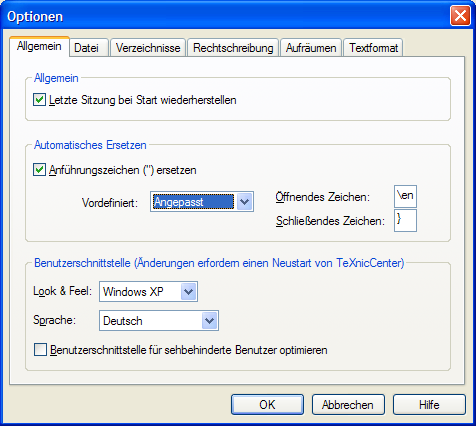
\includegraphics[width=7cm]{images/konfiguration05.png}
		\caption{Konfigurieren der Anf�hrungszeichen}
		\label{fig:konfiguration05}
	\end{center}
\end{figure}

Falls das K�stchen bei \enquote{Anf�hrungszeichen ersetzen} noch nicht markiert ist, markiere es. Danach �nderst du im Pull-Down-Men� den Eintrag auf \enquote{Angepasst} sowie den Eintrag bei \enquote{�ffnendes Anf�hrungszeichen} in \texttt{\textbackslash enquote\{} und bei \enquote{Schlie�endes Anf�hrungszeichen} in \texttt{\}}\footnote{Der Unterschied zwischen den \enquote{Schweizer} und den \foreignquote{french}{Franz�sischen} Anf�hrungszeichen liegt nur im Abstand zwischen Anf�hrungszeichen und Wort. Bei den Schweizer findet sich kein Leerzeichen, bei den Franzosen ein geviert Zwischenraum. Ich verwende in diesem Dokument also die Schweizer, und nicht die Franz�sischen Anf�hrungszeichen.}.

Immer, wenn du jetzt ein einfaches Anf�hrungszeichen (\texttt{''}) eingibst, wird es nun durch ein \textbackslash enquote\{ oder \} ersetzt, je nachdem, ob du dich vor oder hinter einem Wort befindest.

\subsection{Weitere Dokumentation}

Das \enquote{csquotes}-Paket bietet noch eine F�lle an M�glichkeiten, wie zum Beispiel verschiedene Sprachen, Blockquotes und vieles mehr. Die komplette Dokumentation findest du in dem Installationsverzeichniss von MiKTeX unter dem Pfad \enquote{doc\textbackslash latex\textbackslash csquotes}.



% Diplomarbeit mit LaTeX
% ===========================================================================
% This is part of the book "Diplomarbeit mit LaTeX".
% Copyright (c) 2002-2005 Tobias Erbsland, Andreas Nitsch
% See the file diplomarbeit_mit_latex.tex for copying conditions.
%

\chapter{Literaturverzeichnisse und Glossare}
\label{sec:literaturverzeichnisse}

In \DMLLaTeX \ bieten sich zwei unterschiedliche Wege an, Literaturverzeichnisse
anzulegen und zu gestalten. Der einfachere Weg, der allerdings nicht sonderlich
viele Gestaltungsm�glichkeiten offen h�lt, ist die Nutzung der Umgebung \texttt{thebibliography}. Sollen umfangreichere Literaturverzeichnisse oder gar eine Verbindung zu einer Literatur-Datenbank genutzt werden, so
bietet sich das mit \DMLLaTeX \ mitgelieferte Bib\DMLTeX an, zu dessen Nutzung allerdings etwas Einarbeitung notwendig ist.

\section{Einfache Literaturverzeichnisse}
\index{Literaturverzeichnisse!Literaturverzeichnisse@einfache}

Zum Verweisen auf einen Eintrag im Literaturverzeichnis wird sowohl bei der folgenden
einfachen Verzeichniserstellung als auch bei der Erstellung eines Literaturverzeichnisses
mit Bib\DMLTeX der Befehl \texttt{$\backslash$cite\{marke\}} benutzt. Die Variable
\texttt{marke} bezeichnet den Namen des Werkes innerhalb des Literaturverzeichnisses.

Das eigentliche Literaturverzeichnis wird durch Einf�gen der folgenden Umgebung an der
Stelle des Textes, an der es erscheinen soll, eingef�gt:

\begin{verbatim}
      \begin{thebibliography}{defaultmarken}
            \bibitem{marke} Angaben zur Literaturquelle
                .
                .
                .
      \end{theblibliography}
\end{verbatim}

Die angegebene \texttt{defaultmarke} legt die Formatierung der Nummerierung fest.
\newpage

Folgendes Beispiel soll den Einsatz der Umgebung verdeutlichen:

\begin{verbatim}
Was er mit den erbeuteten Knochen zu tun hatte, wusste der
kleine Hund aus einem Buch, dass er in der Stadtb�cherei
gelesen hatte: \emph{"Mein Kochen und ich"} \cite{bjarne}.
Dieses stand dort direkt neben seinem Lieblingsbuch
\emph{"Von Hund zu Hund"} \cite{katz} im B�cherregal
der Hundeliteratur.\\

\begin{thebibliography}{999}
   \bibitem{bjarne} Bjarne Friedjof Blue: "Mein Knochen
   									und ich - wie ich meinen Schatz vergrub"
   \bibitem{katz} Richard Katz: "Von Hund zu Hund"
\end{thebibliography}

\end{verbatim}

Die Ausgabe sieht folgenderma�en aus:

\fbox{\parbox[b]{14.5cm}{
	
	Was er mit den erbeuteten Knochen zu tun hatte, wusste der kleine Hund
	aus einem Buch, dass er in der Stadtb�cherei gelesen hatte:
	\emph{''Mein Kochen und ich''}[1]. Dieses stand dort direkt neben
	seinem Lieblingsbuch \emph{''Von Hund zu Hund''}[2] im B�cherregal
	der Hundeliteratur.
	\vspace{0.5cm}
	\\	
	\Large{Literatur}
	\vspace{1em}
	\\
	\normalsize
	$[$1$]$ Bjarne Friedjof Blue: ''Mein Knochen und ich - wie ich meinen Schatz vergrub''\\
	$[$2$]$ Richard Katz: ''Von Hund zu Hund''
	}
}

\section{Aufwendigere Literaturverzeichnisse}
\index{Literaturverzeichnisse!Literaturverzeichnisse@aufwendigere}
In s�mtlichen wissenschaftlichen Werken, zu denen Diplomarbeiten z�hlen, sollte gro�er Wert auf ein vollst�ndiges und den Normen gen�gendes Literaturverzeichnis gelegt werden. Bib\TeX \ stellt ein �u�erst leistungsf�higes Tool dar, mit dessen Hilfe man automatisch Literaturverzeichnisse erstellen kann.

\subsection{Erstellen der Referenzangaben}
Die eigentlichen Informationen zur verwendeten Literatur werden in einer oder mehreren
separaten Datei(en) mit der Endung \texttt{.bib} abgelegt. Diese Dateien beinhalten f�r
jedes anzugebene Werk einen Eintrag, der je nach Referenzart entsprechende Attribute
besitzt.

Folgend ein Beispiel f�r den Eintrag eines Buches:

\begin{verbatim}
@book{bjarne:knochen,
       author={Bjarne Friedjof Blue},
       title={Mein Knochen und ich - wie ich meinen Schatz
       				vergrub},
       edition={2},
       publisher={Wuff-Verlag},
       isbn={3-12345-6789},
       month={November},
       year={2004},
       language={husky-h�ndisch},
}
\end{verbatim}

Auf dieses Werk w�rde im Text mit der Referenz \verb|\cite{bjarne:knochen}| referenziert
werden.

Als Referenzarten stehen unter anderem folgende Typen zur Verf�gung:

\begin{table}[h]
	\centering
		\begin{tabular}[t]{|l|l|}
		\hline
		@book &Ein von einem Verlag publiziertes Buch\\
		\hline
		@booklet &Gedruckte Arbeit ohne einen Verleger oder eine\\
		 				&publizierende Einrichtung\\
		\hline
		@article &Ein in einem Magazin oder Journal ver�ffentlichter Artikel\\
		\hline
		@inbook &Teil eines Buches, ein Kapitel oder ein bestimmter Bereich\\
						&(Seiten von - bis)\\
		\hline
		@manual &Eine technische Dokumentation\\
		\hline
		@masterthesis &Diplomarbeit\\
		\hline
		@misc &Ein Werk, das in keine andere Kategorie passt\\
		\hline
		\end{tabular}
	\caption{BiB\TeX \ Referenzarten}
	\label{tab:BiBTeXReferenzarten}
\end{table}

\newpage

Je nach Referenzart sind manche Angaben zu einem Werk zwingend erforderlich,
optional oder nicht erforderlich (bei Fehlen gibt \LaTeX \ eine Warnung aus).
Einen �berblick �ber die wichtigsten Attributfelder gibt folgende Tabelle:

\begin{table}[ht]
	\centering
		\begin{tabular}{|l|l|}
			\hline
			author &Name des Autors oder der Autoren\\
			\hline
			booktitle &Titel eines Buches oder eines Buchteils.Zum Verweis auf ein\\
								&ganzes Buch steht das Feld \texttt{title} zur Verf�gung.\\
			\hline
			chapter &Eine Kapitelnummer oder Kapitelbezeichnung.\\
			\hline
			edition &Auflage des Buches, kann eine Zahl oder eine ausgeschriebene Zahl sein.\\
			\hline
			institution &Institution, an der das Werk entstand.\\
			\hline
			journal &Name des Journals oder Magazins.\\
			\hline
			month &Monat der Ver�ffentlichung\\
			\hline
			pages &Eine oder mehrere Seitenzahlen oder -bereiche,\\
						&z.B. 42 -- 50 oder 12, 43, 67.\\
			\hline
			publisher &Name des Verlegers.\\
			\hline
			title &Titel der Arbeit.\\
			\hline
			year &Erscheinungsjahr\\
			\hline
			ISBN &International Standard Book Number\\
			\hline
			language &Sprache, in der das Werk verfasst ist.\\
			\hline
			URL &Universal Ressource Locator, Angabe einer Adresse im Internet\\			
			\hline
		\end{tabular}
	\caption{Literatur-Attributfelder}
	\label{tab:LiteraturAttributfelder}
\end{table}

\subsection{Festlegung des Anzeigestils}
Nachdem die Literaturreferenzen angelegt und in einer oder mehreren Dateien
definiert wurden, k�nnen sie nun unter Angabe eines Anzeigestils, welcher das
genaue Aussehen des Literaturverzeichnisses definiert, in das Hauptdokument eingebunden werden:

\begin{verbatim}
...
\bibliographystyle{geralpha}
\bibliography{name_der_bib_datei_ohne_Endung}
...
\end{verbatim}

\newpage

Eine �bersicht der gebr�uchlichsten Styles f�r deutschsprachige Literaturverzeichnisse
(Pr�fix \textit{ger} steht f�r German) soll folgende Tabelle geben:

\begin{table}[ht]
	\centering
		\begin{tabular}{|l|l|}
			\hline
				gerabbrv &$[$5$]$ Schneider, W.: \emph{Deutsch f�rs Leben - was die Schule zu lehren 				 verga�.}\\
				&\ \ \ \ Rowohlt Taschenbuch Verlag GmbH, Februar 2002.\\
			\hline
				geralpha &$[$Sch02$]$ Schneider, Wolf: \emph{Deutsch f�rs Leben - was die Schule zu
				lehren}\\
				&\ \ \ \ \emph{verga�.} Rowohlt Taschenbuch Verlag GmbH, Februar 2002.\\
			\hline
			  gerapali &$[$Schneider 2002$]$ SCHNEIDER, WOLF (2002). \emph{Deutsch f�rs Leben - 					was}\\
			  &\ \ \ \ \ \emph{die Schule zu lehren verga�.} Rowohlt Taschenbuch Verlag GmbH.\\
			\hline
				gerplain &$[$1$]$ HELMUT SCHAEBEN, MARCUS APEL: \emph{GIS 2D, 3D, 4D, nD.}\\
				&\ \ \ \ \ Informatik Spektrum, Juni 2003.\\
				&\ \ \ \ \ (im Gegensatz zu \texttt{gerabbrv} wird hier nicht nur der erstgenannte\\
				&\ \ \ \ \  Autor aufgef�hrt.\\
			\hline
			  gerunsrt &wie \texttt{gerabbrv}, allerdings werden die Werke nicht alphabetisch nach\\
			  &\ \ \ \ \  Autor sortiert, sondern wie in der bib-Datei aufgef�hrt aufgelistet.\\
			  \hline
		\end{tabular}
	\caption{Style �bersicht}
	\label{tab:style_uebersicht}
\end{table}

Um diese Styles nutzen zu k�nnen, mu� das Paket \textit{germbib} installiert sein (bei MiKTeX-Standardinstallation der Fall) und \textit{bibgerm.sty} mit \textbackslash usepackage\{bibgerm\} im Dokumentenkopf eingebunden werden.

Wer mit den gegebenen Standard-Styles nicht zufrieden ist, der kann sich auch seinen
eigenen Bib\TeX-Style erstellen. Dieses zu schildern w�rde hier allerdings den Rahmen
sprengen, deshalb sei hier nur auf das Tutorium von Bernd Raichle \cite{raichle:bibtex_programmierung} verwiesen.

\subsection{Einbinden der Referenzen in den Text und Erstellung des
Literaturverzeichnisses}
Nachdem die eigentlichen Angaben zur verwendeten Literatur in der .bib-Datei
angelegt worden sind, m�ssen diese Angaben noch mit den passenden Stellen im
Text, an denen das Werk zitiert wird, verkn�pft werden.
Hierzu wird der Befehl \texttt{cite{}}(f�r citation) verwendet:
\begin{verbatim}
	N�here Informationen finden sich im Buch "Mein Knochen und ich -
	wie ich meinen Schatz vergrub" \cite{bjarne:knochen}
\end{verbatim}
\newpage
Die Ausgabe sieht, je nach Einstellung des Anzeigestiles (s. hierzu Tabelle
\ref{tab:style_uebersicht}) etwa wie folgt aus:
\begin{verbatim}
	N�here Informationen finden sich im Buch "Mein Knochen und ich -
	wie ich meinen Schatz vergrub" [Bjar05].
\end{verbatim}
Um das eigentliche Literaturverzeichnis zu erstellen und einzubinden, ist folgendes Vorgehen
n�tig:

Zuerst l�sst man einen \DMLLaTeX-Lauf �ber das gesamte Dokument laufen, wodurch
f�r jede Datei der Projektes eine zugeh�rige Datei mit der Endung \texttt{.aux}
erstellt wird. In diesen Dateien sind unter anderem die Literatureintr�ge
verzeichnet, auf die in dem jeweiligen Dokument verwiesen wird.
Anschlie�end wird das Programm \texttt{Bib\DMLTeX} aufgerufen, welches diese Eintr�ge
sammelt, sortiert und in eine Datei mit der Endung \texttt{.bbl} schreibt.
Bib\DMLTeX kann im \DMLTeX nicCenter sehr bequem �ber den Men�punkt \texttt{Ausgabe
$\rightarrow$ Bib\DMLTeX} aufgerufen werden. Nach einem weiteren \DMLLaTeX-Lauf wird
das fertig sortierte und formatierte Literaturverzeichnisse in das Dokument
eingebunden.

Falls dir das dauernde Aufrufen von \DMLLaTeX \ bzw. Pdf\DMLTeX \ und die Aufrufe von
Bib\DMLTeX und makeindex (s. hierzu Kapitel \ref{sec:glossar}) zuviel wird, kannst du diese
Arbeitsschritte auch �ber eine Befehlsdatei, ein sogenanntes \texttt{Batchscript}
automatisieren. Ein Beispiel f�r eine solche Batchdatei findet sich in Listing
\ref{subsec:batchdatei}.

%
% Diplomarbeit mit LaTeX
% ===========================================================================
% This is part of the book "Diplomarbeit mit LaTeX".
% Copyright (c) 2002, 2003, 2005 Tobias Erbsland, Andreas Nitsch
% See the file main.tex for copying conditions.
%

\section{Glossare}
\label{sec:glossar}

Bei größeren Dokumenten, insbesondere zu komplexen Themen, kann es recht
sinnvoll sein, Begriffe, die nicht jedem geläufig sind und oft benutzt
werden, gesondert zu erklären.

Selbst beim Schreiben einer Diplomarbeit kann es für den Autor selbst
sehr sinnvoll sein, Begrifflichkeiten zu erklären, um sich selber vollständig
über ihre Bedeutung klar zu werden. Dem Leser jedenfalls wird mit einem Glossar
unter Umständen eine große (Verständnis-) Hilfe geboten und lästiges
Durchsuchen der gesamten Arbeit nach einer Begriffserklärung wird vermieden.
\vspace{1em}
\\
Zum Erstellen eines Glossars gehören, wie beim Erstellen des Literaturverzeichnisses,
 prinzipiell drei Schritte.
Im ersten Schritt werden die einzelnen Glossareinträge innerhalb des Textes
angelegt. Durch einen \DMLLaTeX-Lauf werden diese Glossareinträge in
einer Datei mit der Endung ''.glo'' gesammelt, durch den Aufruf des
Zusatzprogrammes \emph{makeindex} sortiert und in das \DMLLaTeX-Dokument
eingebunden. Durch einen weiteren \DMLLaTeX-Lauf wird hiernach das fertige
Dokument erzeugt.
\vspace{1em}
\\
Die Glossareinträge können an jeder beliebigen Stelle eines Dokumentes erstellt werden.
Die Definition erfolgt durch den Befehl \texttt{glossary}:
\begin{verbatim}
	\glossary{
						name={Knochen},
						description={Lieblingsspeise eines jeden Hundes. Besonderer
												 Beliebtheit erfreuen sich Rinderknochen.}
	}
\end{verbatim}
Nach einem  \DMLLaTeX-Durchlauf  werden die Zwischendateien mit den Endungen ''.glo'' und
''.ist''erzeugt, welche die aus den Dateien extrahierten Einträgen bzw. die
Formatierungsbeschreibung des Glossars enthalten. Um diese Formatierung auf die extrahierten
Einträge anzuwenden, wird das Programm \texttt{makeindex} benutzt, dessen Aufruf leider
etwas langatmig ist. In der Windows-Eingabeaufforderung (Start $\rightarrow$ Alle Programme
$\rightarrow$ Zubehör $\rightarrow$ Eingabeaufforderung) ist folgende Kommandozeile einzugeben:
\begin{verbatim}
		makeindex -s diplomarbeit_akki.ist -t diplomarbeit_akki.glg -o
								 diplomarbeit_akki.gls diplomarbeit_akki.glo
\end{verbatim}
Makeindex erzeugt eine Datei mit der Endung ''.gls'', in welcher das fertig formatierte Glossar
enthalten ist. Dieses kann mit dem Befehl
\begin{verbatim}
	\renewcommand{\glossaryname}{Glossar}
	\printglossary
\end{verbatim}
an jeder beliebigen Stelle der Diplomarbeit eingefügt werden und wird dort nach einem weiteren
\DMLLaTeX-Lauf ausgegeben. Das Kommando \texttt{renewcommand} dient an dieser Stelle dazu, die
automatisch eingefügte Überschrift des Glossars neu zu setzen, da diese standardmäßig auf
englich erscheint (''Glossary'') und bei einer deutschsprachigen Diplomarbeit besser in deutsch
gehalten sein sollte.

Ein Beispiel für das Einbinden eines Glossars findet sich in Listing
\ref{subsec:listing_hauptdokument}, ein Beispiel für das Anlegen von Glossareinträgen in Listing
\ref{subsec:zweites_kapitel} und zum automatisierten Ablauf des Übersetzungsvorganges wird auf
die Batchdatei in Listing \ref{subsec:batchdatei} verwiesen.

\subsection{Formatierungsmöglichkeiten des Glossars}
Neben der Änderung der Glossarüberschrift gibt es noch weitere Einstellungen, mit denen man das
Aussehen des Glossars beeinflussen kann. Folgende Einstellungen können im Header vorgenommen
(s. Listing \ref{subsec:header}) werden und bestimmen, wie das glossary-Paket angewendet wird:

\begin{tabularx}{\textwidth}{lX}
			style &Der Glossar-Stil. Mögliche Werte sind:\\
						&\textbf{list}: stellt Begriffe (fettgedruckt) und Erklärung in einer Zeile dar.\\
						&\textbf{altlist}: stellt den Begriff fettgedruckt dar, Erklärung folgt versetzt auf der nächsten Zeile\\
						&\textbf{super}: nutzt die \texttt{supertabular}- Umgebung für das Glossar.\\
						&\textbf{long}: nutzt die \texttt{longtable}- Umgebung für das Glossar (default).\\
			header &Setzt die Überschriften der Begriffs- und Erklärungsspalten. Mögliche Werte sind:\\
					  &\textbf{none}: Spalten haben keine Überschriften (default).\\
					  &\textbf{plain}: Spalten haben Überschriften.\\
		  border &Rahmen um das Glossar. Mögliche Werte sind:\\
		  			&\textbf{none}: Glossar ist nicht eingerahmt (default).\\
		  			&\textbf{plain}: Körper des Glossars wird eingerahmt.\\		  
			cols	& Anzahl der Spalten des Glossars. Mögliche Werte sind:\\ 
						&\textbf{2}: Die Begriffsbezeichnung ist in der ersten, Erklärung und zugehörige Seitenzahl in der zweiten Glossarspalte (default).\\ 
						&\textbf{3}: Die Begriffsbezeichnung ist in der ersten, die Erklärung in der zweiten und die zugehörigen Seitenzahlen in der dritten Glossarspalte.\\
		  number &Die jedem Eintrag zugeordnete Nummerierung. Nummerierungen können sein:\\
		  			&\textbf{page}: jedem Eintrag sind/ist die zugehörige(n) Seitenzahl(en) zugeordnet (default).\\
		  			&\textbf{section}: jedem Eintrag sind/ist die zugehörige(n) Kapitelnummer(n) zugeordnet.\\
		  			&\textbf{none}: es werden den Einträgen keine Nummerierung hinzugefügt.\\
		  toc &Legt fest, ob das Glossar in das Inhaltsverzeichnis aufgenommen werden soll:\\
		  		&\textbf{true}: fügt das Glossar zum Inhaltsverzeichnis hinzu.\\
		  		&\textbf{false}: fügt das Glossar nicht zum Inhaltsverzeichnis hinzu.
\end{tabularx}
\vspace{1em}
\\
Weitere Möglichkeiten, Glossare nach eigenen Vorstellungen zu gestalten, finden sich im
Dokument ''glossary.dvi -- glossary.sty: \DMLLaTeX \ Package to Assist Generating Glossaries''\footnote{Dieses Dokument befindet sich im Mik\TeX"=Verzeichnis: \verb~/miktex/doc/latex/glossary~.}. 
Als durchaus optisch ansprechend und übersichtlich haben sich die Glossar"=Einstellungen erwiesen, wie sie im Beispiellisting \ref{subsec:header} angeführt sind.

%%
% Diplomarbeit mit LaTeX
% ===========================================================================
% This is part of the book "Diplomarbeit mit LaTeX".
% Copyright (c) 2002, 2003, 2005 Tobias Erbsland, Andreas Nitsch
% See the file main.tex for copying conditions.
%

\chapter{Verwenden von eigenen Schriften}

(in Arbeit)

%\include{chapters/latex2rtf}
%\include{chapters/beamerfolien_mit_latex}

% Diplomarbeit mit LaTeX
% ===========================================================================
% This is part of the book "Diplomarbeit mit LaTeX".
% Copyright (c) 2002-2005, 2007 Tobias Erbsland
% Copyright (c) 2005 Andreas Nitsch
% See the file diplomarbeit_mit_latex.tex for copying conditions.
%

\chapter{Literaturempfehlungen}
\index{Literatur}\index{Bucher@Bücher}

\section{Bücher und Internetadressen}

Setzt du konsequent die Hilfsmittel ein, die \DMLLaTeX{} dir bietet, so wirst du auf jeden Fall ein optisch ansprechendes Dokument erhalten. Wenn du dabei auch noch die Regeln beachtest und dich um Warnungen und Fehlermeldungen kümmerst, dann erhälst du ein optisch überzeugendes Dokument.

Ob deine Diplomarbeit für den Leser besonders spannend ist, hängt sowohl vom jeweiligen Thema und von den Interessen des Lesers ab. Trotzdem kannst du noch einiges optimieren um deine Arbeit für den Leser\footnote{Besonders für diejenigen, die dir eine Note dafür geben werden} spannender und sicher auch unterhaltsamer zu gestalten.

Mit \enquote{einfachen Wörtern} und \enquote{schönen Sätzen} kann der Leser dein Werk in vollen Zügen genießen.

Falls aber Schreiben nicht zu deinem Stärken zählt, könnten dir die folgenden Literaturtipps eine gute Hilfe sein. Einige davon kannst du kostenlos über das Internet beziehen.

\begin{itemize}
	\item{Claudia Fritsch: ''Schreiben für die Leser''\cite{fritsch:schreiben_fuer_die_Leser}}
	\item{Wolf Schneider: ''Deutsch fürs Leben''\cite{schneider:deutsch_fuers_leben}}
\end{itemize}

Weitere und ausführlichere \footnote{...dafür aber nicht so speziell auf das Erstellen einer Diplomarbeit ausgelegte} Literatur zu \DMLLaTeX{} findest du  kostenlos im Internet:

\begin{itemize}
	\item{Manuela Jürgens: \enquote{\DMLLaTeX{} -- eine Einführung und ein bisschen mehr}\cite{juergens:latex1}}
	\item{Manuela Jürgens: \enquote{\DMLLaTeX{} -- fortgeschrittene Anwendungen}\cite{juergens:latex2}}
\end{itemize}

Zudem gibt es viele gute Bücher welche weitere Details von \DMLLaTeX{} beschreiben. Folgende Bücher können als Standardwerke in Sachen \LaTeX \ bezeichnet werden:

\begin{itemize}
	\item{Frank Mittelback, Michael Goossens: \enquote{Der \DMLLaTeX"=Begleiter}\cite{DerLaTeXBegleiter}}
	\item{Helmut Kopka: \enquote{\DMLLaTeX: Band 1 - Eine Einführung}\cite{kopka:band1}}
	\item{Helmut Kopka: \enquote{\DMLLaTeX: Band 2 - Ergänzungen}\cite{kopka:band2}}
	\item{Helmut Kopka: \enquote{\DMLLaTeX: Band 3 - Erweiterungen}\cite{kopka:band3}}
	\item{Leslie Lamport: \enquote{\DMLLaTeX, A Document Preparation System, User's Guide and Reference Manual}\cite{lamport:latex}}
\end{itemize}





\appendix
%
% Abschlussarbeit mit LaTeX
% ===========================================================================
% This is part of the book "Abschlussarbeit mit LaTeX".
% Copyright (c) 2002-2008 Tobias Erbsland, Andreas Nitsch
% See the file abschlussarbeit_mit_latex.tex for copying conditions.
%

\chapter{Ausstehendes und offene Fragen}
\label{sec:ausstehendes}

\section{Ausstehende Punkte}

Hier werden unsortiert alle Fragen und ausstehende Punkte aufgelistet, welche noch zu beantworten oder zu realisieren sind. Falls du mich bei einem dieser Punkte unterstützen kannst, würde ich mich über deine Mitarbeit freuen.

\begin{itemize}
	\item Ein Kapitel über Querverweise.
	\item Eine Erklärung zu den Paketen \textbackslash use\-package\{mathptmx\},\\ \textbackslash usepackage[scaled=.92]\{helvet\} und \textbackslash usepackage\{courier\}, sowie über die
	Vor- und Nachteile dieser Pakete bei der Darstellung eines PDF-Dokumentes.
	\item Hinweis auf die Koma-Script-Dokumentation \enquote{scrguide} deutlicher unterbringen (genauer Platz innerhalb der MikTeX-Verzeichnisstruktur).
	\item Eine Erklärung zur Option \enquote{\!} bei Floats, sowie einen Hinweis darauf, dass Floats ohne Optionen auch sehr gut platziert werden.
	\item Bei den Grundlagen wird in \cref{Sonderzeichen} gesagt, wie man die reservierten Sonderzeichen benutze, werde später gesagt - wo? Außerdem fehlt eine kurze Erklärung, wofür welches Zeichen steht, also Tilde für geschütztes Leerzeichen etc.
\end{itemize}

\section{Ankündigungen}

Des Weiteren möchte Andreas weitere Kapitel hinzufügen (wird wohl im Laufe seiner eigenen Diplomarbeit
in kurzer Zeit geschehen):

\begin{itemize}
	\item Das Erstellen von Präsentationen in Form von Beamerfolien mit der ''beamer''-Klasse
	\item Konvertieren von \DMLLaTeX"=Dokumenten ins rtf-Format mittels rtf3\DMLLaTeX.
\end{itemize}

\section{Hilfe gesucht}
\label{sec:hilfe-gesucht}

Für die folgenden Aufgaben suche ich noch Leute, die mich unterstützen. Kontaktiere mich per Mail, falls du eine der folgenden Aufgaben gerne lösen möchtest. Du erhältst dann Zugang zum Versionsverwaltungssystem dieses Dokuments und kannst so deinen Teil zu diesem Dokument beitragen.

\begin{itemize}
	\item Viele Leute haben mir bereits komplette Korrekturen der PDF Version geschickt. Nochmals Vielen Dank an dieser Stelle für
	diese Korrekturen. Um die Fehler jedoch alle im Quellcode zu finden und zu korrigieren, fehlt mir einfach die Zeit. Wer mag, kann
	das Dokument verbessern, indem er alle Rechtschreibfehler korrigiert. Dies jedoch direkt im Quellcode, nicht im PDF.
	\item Es fehlen auch noch viele andere Kapitel. Vielleicht möchtest du ja noch eines schreiben.
\end{itemize}

Über die URL \href{https://secure.drzoom.ch/svn/dml}{https://secure.drzoom.ch/svn/dml} kannst du mit \enquote{Subversion} jederzeit die Quellen der aktuellste Version des Dokuments holen und deine Änderungen einarbeiten. Um deine Änderungen hochzuladen, benötigst du einen Account. Diesen bekommst du bei mir (Tobias). Schreib mir dazu einfach ein Mail, beschreib kurz was du gerne hinzufügen möchtest und wie dein Accountname heissen soll.

Ein guter Subversion Client für Windows ist \href{http://tortoisesvn.tigris.org/}{\enquote{TortoiseSVN}}. Weitere Informationen über Subversion findest du im \href{http://svnbook.red-bean.com/}{\enquote{Subversion Book}}.


%
% Diplomarbeit mit LaTeX
% ===========================================================================
% This is part of the book "Diplomarbeit mit LaTeX".
% Copyright (c) 2002-2005 Tobias Erbsland, Andreas Nitsch
% See the file diplomarbeit_mit_latex.tex for copying conditions.
%

\chapter{Listings}

\section{Beispiellisting eines Dokuments mit der Dokumentklasse \enquote{scrartcl}}
\label{sec:lstarticle}

\lstinputlisting[caption=Beispiellisting eines Dokuments mit der Dokumentklasse \enquote{scrartcl}, label=lst:article, frame=tb]%
	{listings/beispiel02.tex}
	
\section{Beispiellisting eines Dokuments mit der Dokumentklasse \enquote{scrreprt}}
\label{sec:lstreport}

\lstinputlisting[caption=Beispiellisting eines Dokuments mit der Dokumentklasse \enquote{scrartcl}, label=lst:report, frame=tb]%
	{listings/beispiel03.tex}
	
\section{Beispiellisting eines Dokuments mit der Dokumentklasse \enquote{scrbook}}
\label{sec:lstbook}

\lstinputlisting[caption=Beispiellisting eines Dokuments mit der Dokumentklasse \enquote{scrbook}, label=lst:book, frame=tb]%
	{listings/beispiel04.tex}

\newpage	
\section{Beispiellisting einer Diplomarbeit}
\label{sec:listing_diplomarbeit}

\subsection{Hauptdokument einer Diplomarbeit}
\label{subsec:listing_hauptdokument}

\lstinputlisting[caption=Hauptdokument der Diplomarbeit, label=lst:hauptdokument, frame=tb]
	{template_diplomarbeit/template_diplomarbeit.tex}


\newpage	
\subsection{Header Diplomarbeit}
\label{subsec:header}

\lstinputlisting[caption=Header der Diplomarbeit, label=lst:header, frame=tb]
	{template_diplomarbeit/kapitel/header.tex}


\newpage
\subsection{Titelseite der Diplomarbeit}
%\label{subsec:titelseite}

\lstinputlisting[caption=Titelseite der Diplomarbeit, label=lst:titelseite, frame=tb]
	{template_diplomarbeit/kapitel/titelseite.tex}


\newpage	
\subsection{Einleitung der Diplomarbeit}
%\label{subsec:einleitung}

\lstinputlisting[caption=Einleitung der Diplomarbeit, label=lst:einleitung, frame=tb]
	{template_diplomarbeit/kapitel/abstract.tex}

\subsection{Danksagung zur Diplomarbeit}
%\label{subsec:danksagung}

\lstinputlisting[caption=Danksagung Diplomarbeit, label=lst:danksagung,
 frame=tb]
	{template_diplomarbeit/kapitel/danksagung.tex}


\newpage
\subsection{Erstes Kapitel der Diplomarbeit}
%\label{subsec:erstes_kapitel}

\lstinputlisting[caption=Erstes Kapitel der Diplomarbeit - ohne Glossareintr�ge, label=lst:erstes_kapitel,
 frame=tb]
	{template_diplomarbeit/kapitel/charakteristik_spuerhund.tex}

\subsection{Zweites Kapitel der Diplomarbeit}
\label{subsec:zweites_kapitel}

\lstinputlisting[caption=Zweites Kapitel der Diplomarbeit - mit Glossareintr�ge, label=lst:zweites_kapitel,
 frame=tb]
	{template_diplomarbeit/kapitel/zukunftsaussichten_spuerhund.tex}

\newpage
\subsection{Eidesstattliche Erkl�rung zur Diplomarbeit}
\label{subsec:eidesstatt}
\lstinputlisting[caption=Eidesstattliche Erkl�rung -- an Hochschul-Bedingungen anzupassen, label=lst:eidesstattliche_erklaerung,
 frame=tb]
	{template_diplomarbeit/kapitel/eidesstattliche_erklaerung.tex}


\newpage
\subsection{Batchdatei zum �bersetzen des LaTeX-Dokumentes}
\label{subsec:batchdatei}
\lstinputlisting[caption=Batchdatei zum �bersetzen des \DMLLaTeX-Dokumentes, label=lst:batchdatei,
 frame=tb]
	{template_diplomarbeit/make.bat}	
	
%
% EOF
%

%
% Diplomarbeit mit LaTeX
% ===========================================================================
% This is part of the book "Diplomarbeit mit LaTeX".
% Copyright (c) 2002-2005 Tobias Erbsland, Andreas Nitsch
% See the file diplomarbeit_mit_latex.tex for copying conditions.
%

\chapter{Tastenkombinationen im TeXnicCenter}

Hier noch die wichtigsten Tastenkombinationen für eine schnelle Bedienung vom TeXnicCenter. Die Tastenkommandos lassen sich natürlich anpassen. Über das Hilfemenü \enquote{?} $\Rightarrow$ \enquote{Tastaturbelegung...} lässt sich die Tastaturbelegung auch anzeigen oder ausdrucken. 

\begin{table}
	\begin{center}
	\begin{tabular}{rl}
		\textbf{Tastenkombination} & \textbf{Beschreibung} \\ \hline
		
		Ctrl + 0-9 & Setzen von nummeriertem Lesezeichen \\
		Alt + 0-9 & Zu nummerierten Lesezeichen springen \\
		
		Ctrl + A & Markiert das ganze Dokument \\
		Ctrl + Alt + A & Einfügen einer Abbildungsumgebung \\
		
		Ctrl + B & Gehe zu letzter Änderung \\
		Ctrl + Alt + B & Einfügen einer Beschreibungsliste \\
		
		
		Ctrl + C & Markierten Text in die Zwischenablage kopieren \\
		
		
		Ctrl + E & Hervorheben des markierten Textes \\
		Ctrl + Alt + E & Einfügen eines Aufzählungseintrags \\
		
		Ctrl + F & Suchen eines Textes \\
		Ctrl + Alt + F & Einfügen einer Fußnote \\
		
		Ctrl + Alt + G & Einfügen einer Grafik (Dialog) \\
		
		Ctrl + H & Ersetzen eines Textes \\
		
		Ctrl + K & Kursivsetzen des markierten Textes \\
	
		Ctrl + Alt + L & Einfügen eines Beschreibungsbeitrags \\
	
		Ctrl + Alt + N & Einfügen einer Nummerierung \\
		
	
		Ctrl + S & Speichen des aktuellen Dokuments \\
		Ctrl + Shift + S & Speichern aller Dokumente \\
		Ctrl + Alt + S & Erzeugen eines neuen Titels \\
		
		Ctrl + Alt + T & Einfügen einer Tabelle (Dialog) \\
		
		Ctrl + V & Text aus Zwischenablage einfügen \\
		
		Ctrl + X & Markierten Text ausschneiden und in die Zwischenablage \\
		
		Ctrl + Z & Undo, macht die letzte Aktion Rückgängig \\
		Ctrl + Alt + Z & Einfügen einer Aufzählung \\	
		
		F3 & Nach suchen, zum nächsten Treffer springen \\
		
		F5 & Ausgabedatei Betrachten \\
		F7 & Projekt Kompilieren \\
		Ctrl + F7 & Aktuelle Datei kompilieren \\
		
		F9 & Nächster Fehler anzeigen \\
		Shift + F9 & Vorheriger Fehler anzeigen \\
			
		F10 & Nächste Warnung anzeigen \\
		Shift + F10 & Vorherige Warnung anzeigen \\

		F11 & Nächste volle/leere Box anzeigen \\
		Shift + F11 & Vorherige volle/leere Box anzeigen \\
	\end{tabular}
	\end{center}
	\caption{Tastenkombinationen im TeXnicCenter}
\end{table}

%
% Diplomarbeit mit LaTeX
% ===========================================================================
% This is part of the book "Diplomarbeit mit LaTeX".
% Copyright (c) 2002-2005 Tobias Erbsland, Andreas Nitsch
% See the file diplomarbeit_mit_latex.tex for copying conditions.
%

\chapter{GNU Free Documentation License}

Version 1.2, November 2002

 Copyright (C) 2000,2001,2002  Free Software Foundation, Inc.
     59 Temple Place, Suite 330, Boston, MA  02111-1307  USA
 Everyone is permitted to copy and distribute verbatim copies
 of this license document, but changing it is not allowed.


\section*{Preamble}

The purpose of this License is to make a manual, textbook, or other
functional and useful document \enquote{free} in the sense of freedom: to
assure everyone the effective freedom to copy and redistribute it,
with or without modifying it, either commercially or noncommercially.
Secondarily, this License preserves for the author and publisher a way
to get credit for their work, while not being considered responsible
for modifications made by others.

This License is a kind of \enquote{copyleft}, which means that derivative
works of the document must themselves be free in the same sense.  It
complements the GNU General Public License, which is a copyleft
license designed for free software.

We have designed this License in order to use it for manuals for free
software, because free software needs free documentation: a free
program should come with manuals providing the same freedoms that the
software does.  But this License is not limited to software manuals;
it can be used for any textual work, regardless of subject matter or
whether it is published as a printed book.  We recommend this License
principally for works whose purpose is instruction or reference.


\section*{Applicability and definitions}

This License applies to any manual or other work, in any medium, that
contains a notice placed by the copyright holder saying it can be
distributed under the terms of this License.  Such a notice grants a
world-wide, royalty-free license, unlimited in duration, to use that
work under the conditions stated herein.  The \enquote{Document}, below,
refers to any such manual or work.  Any member of the public is a
licensee, and is addressed as \enquote{you}.  You accept the license if you
copy, modify or distribute the work in a way requiring permission
under copyright law.

A \enquote{Modified Version} of the Document means any work containing the
Document or a portion of it, either copied verbatim, or with
modifications and/or translated into another language.

A \enquote{Secondary Section} is a named appendix or a front-matter section of
the Document that deals exclusively with the relationship of the
publishers or authors of the Document to the Document's overall subject
(or to related matters) and contains nothing that could fall directly
within that overall subject.  (Thus, if the Document is in part a
textbook of mathematics, a Secondary Section may not explain any
mathematics.)  The relationship could be a matter of historical
connection with the subject or with related matters, or of legal,
commercial, philosophical, ethical or political position regarding
them.

The \enquote{Invariant Sections} are certain Secondary Sections whose titles
are designated, as being those of Invariant Sections, in the notice
that says that the Document is released under this License.  If a
section does not fit the above definition of Secondary then it is not
allowed to be designated as Invariant.  The Document may contain zero
Invariant Sections.  If the Document does not identify any Invariant
Sections then there are none.

The \enquote{Cover Texts} are certain short passages of text that are listed,
as Front-Cover Texts or Back-Cover Texts, in the notice that says that
the Document is released under this License.  A Front-Cover Text may
be at most 5 words, and a Back-Cover Text may be at most 25 words.

A \enquote{Transparent} copy of the Document means a machine-readable copy,
represented in a format whose specification is available to the
general public, that is suitable for revising the document
straightforwardly with generic text editors or (for images composed of
pixels) generic paint programs or (for drawings) some widely available
drawing editor, and that is suitable for input to text formatters or
for automatic translation to a variety of formats suitable for input
to text formatters.  A copy made in an otherwise Transparent file
format whose markup, or absence of markup, has been arranged to thwart
or discourage subsequent modification by readers is not Transparent.
An image format is not Transparent if used for any substantial amount
of text.  A copy that is not \enquote{Transparent} is called \enquote{Opaque}.

Examples of suitable formats for Transparent copies include plain
ASCII without markup, Texinfo input format, LaTeX input format, SGML
or XML using a publicly available DTD, and standard-conforming simple
HTML, PostScript or PDF designed for human modification.  Examples of
transparent image formats include PNG, XCF and JPG.  Opaque formats
include proprietary formats that can be read and edited only by
proprietary word processors, SGML or XML for which the DTD and/or
processing tools are not generally available, and the
machine-generated HTML, PostScript or PDF produced by some word
processors for output purposes only.

The \enquote{Title Page} means, for a printed book, the title page itself,
plus such following pages as are needed to hold, legibly, the material
this License requires to appear in the title page.  For works in
formats which do not have any title page as such, \enquote{Title Page} means
the text near the most prominent appearance of the work's title,
preceding the beginning of the body of the text.

A section \enquote{Entitled XYZ} means a named subunit of the Document whose
title either is precisely XYZ or contains XYZ in parentheses following
text that translates XYZ in another language.  (Here XYZ stands for a
specific section name mentioned below, such as \enquote{Acknowledgements},
\enquote{Dedications}, \enquote{Endorsements}, or \enquote{History}.)  To \enquote{Preserve the Title}
of such a section when you modify the Document means that it remains a
section \enquote{Entitled XYZ} according to this definition.

The Document may include Warranty Disclaimers next to the notice which
states that this License applies to the Document.  These Warranty
Disclaimers are considered to be included by reference in this
License, but only as regards disclaiming warranties: any other
implication that these Warranty Disclaimers may have is void and has
no effect on the meaning of this License.


\section*{Verbatim copying}

You may copy and distribute the Document in any medium, either
commercially or noncommercially, provided that this License, the
copyright notices, and the license notice saying this License applies
to the Document are reproduced in all copies, and that you add no other
conditions whatsoever to those of this License.  You may not use
technical measures to obstruct or control the reading or further
copying of the copies you make or distribute.  However, you may accept
compensation in exchange for copies.  If you distribute a large enough
number of copies you must also follow the conditions in section 3.

You may also lend copies, under the same conditions stated above, and
you may publicly display copies.


\section*{Copying in quantity}

If you publish printed copies (or copies in media that commonly have
printed covers) of the Document, numbering more than 100, and the
Document's license notice requires Cover Texts, you must enclose the
copies in covers that carry, clearly and legibly, all these Cover
Texts: Front-Cover Texts on the front cover, and Back-Cover Texts on
the back cover.  Both covers must also clearly and legibly identify
you as the publisher of these copies.  The front cover must present
the full title with all words of the title equally prominent and
visible.  You may add other material on the covers in addition.
Copying with changes limited to the covers, as long as they preserve
the title of the Document and satisfy these conditions, can be treated
as verbatim copying in other respects.

If the required texts for either cover are too voluminous to fit
legibly, you should put the first ones listed (as many as fit
reasonably) on the actual cover, and continue the rest onto adjacent
pages.

If you publish or distribute Opaque copies of the Document numbering
more than 100, you must either include a machine-readable Transparent
copy along with each Opaque copy, or state in or with each Opaque copy
a computer-network location from which the general network-using
public has access to download using public-standard network protocols
a complete Transparent copy of the Document, free of added material.
If you use the latter option, you must take reasonably prudent steps,
when you begin distribution of Opaque copies in quantity, to ensure
that this Transparent copy will remain thus accessible at the stated
location until at least one year after the last time you distribute an
Opaque copy (directly or through your agents or retailers) of that
edition to the public.

It is requested, but not required, that you contact the authors of the
Document well before redistributing any large number of copies, to give
them a chance to provide you with an updated version of the Document.


\section*{Modifications}

You may copy and distribute a Modified Version of the Document under
the conditions of sections 2 and 3 above, provided that you release
the Modified Version under precisely this License, with the Modified
Version filling the role of the Document, thus licensing distribution
and modification of the Modified Version to whoever possesses a copy
of it.  In addition, you must do these things in the Modified Version:

\begin{description}
\item[A.] Use in the Title Page (and on the covers, if any) a title distinct
   from that of the Document, and from those of previous versions
   (which should, if there were any, be listed in the History section
   of the Document).  You may use the same title as a previous version
   if the original publisher of that version gives permission.
\item[B.] List on the Title Page, as authors, one or more persons or entities
   responsible for authorship of the modifications in the Modified
   Version, together with at least five of the principal authors of the
   Document (all of its principal authors, if it has fewer than five),
   unless they release you from this requirement.
\item[C.] State on the Title page the name of the publisher of the
   Modified Version, as the publisher.
\item[D.] Preserve all the copyright notices of the Document.
\item[E.] Add an appropriate copyright notice for your modifications
   adjacent to the other copyright notices.
\item[F.] Include, immediately after the copyright notices, a license notice
   giving the public permission to use the Modified Version under the
   terms of this License, in the form shown in the Addendum below.
\item[G.] Preserve in that license notice the full lists of Invariant Sections
   and required Cover Texts given in the Document's license notice.
\item[H.] Include an unaltered copy of this License.
\item[I.] Preserve the section Entitled \enquote{History}, Preserve its Title, and add
   to it an item stating at least the title, year, new authors, and
   publisher of the Modified Version as given on the Title Page.  If
   there is no section Entitled \enquote{History} in the Document, create one
   stating the title, year, authors, and publisher of the Document as
   given on its Title Page, then add an item describing the Modified
   Version as stated in the previous sentence.
\item[J.] Preserve the network location, if any, given in the Document for
   public access to a Transparent copy of the Document, and likewise
   the network locations given in the Document for previous versions
   it was based on.  These may be placed in the \enquote{History} section.
   You may omit a network location for a work that was published at
   least four years before the Document itself, or if the original
   publisher of the version it refers to gives permission.
\item[K.] For any section Entitled \enquote{Acknowledgements} or \enquote{Dedications},
   Preserve the Title of the section, and preserve in the section all
   the substance and tone of each of the contributor acknowledgements
   and/or dedications given therein.
\item[L.] Preserve all the Invariant Sections of the Document,
   unaltered in their text and in their titles.  Section numbers
   or the equivalent are not considered part of the section titles.
\item[M.] Delete any section Entitled \enquote{Endorsements}.  Such a section
   may not be included in the Modified Version.
\item[N.] Do not retitle any existing section to be Entitled \enquote{Endorsements}
   or to conflict in title with any Invariant Section.
\item[O.] Preserve any Warranty Disclaimers.
\end{description}

If the Modified Version includes new front-matter sections or
appendices that qualify as Secondary Sections and contain no material
copied from the Document, you may at your option designate some or all
of these sections as invariant.  To do this, add their titles to the
list of Invariant Sections in the Modified Version's license notice.
These titles must be distinct from any other section titles.

You may add a section Entitled \enquote{Endorsements}, provided it contains
nothing but endorsements of your Modified Version by various
parties--for example, statements of peer review or that the text has
been approved by an organization as the authoritative definition of a
standard.

You may add a passage of up to five words as a Front-Cover Text, and a
passage of up to 25 words as a Back-Cover Text, to the end of the list
of Cover Texts in the Modified Version.  Only one passage of
Front-Cover Text and one of Back-Cover Text may be added by (or
through arrangements made by) any one entity.  If the Document already
includes a cover text for the same cover, previously added by you or
by arrangement made by the same entity you are acting on behalf of,
you may not add another; but you may replace the old one, on explicit
permission from the previous publisher that added the old one.

The author(s) and publisher(s) of the Document do not by this License
give permission to use their names for publicity for or to assert or
imply endorsement of any Modified Version.


\section*{Combining documents}

You may combine the Document with other documents released under this
License, under the terms defined in section 4 above for modified
versions, provided that you include in the combination all of the
Invariant Sections of all of the original documents, unmodified, and
list them all as Invariant Sections of your combined work in its
license notice, and that you preserve all their Warranty Disclaimers.

The combined work need only contain one copy of this License, and
multiple identical Invariant Sections may be replaced with a single
copy.  If there are multiple Invariant Sections with the same name but
different contents, make the title of each such section unique by
adding at the end of it, in parentheses, the name of the original
author or publisher of that section if known, or else a unique number.
Make the same adjustment to the section titles in the list of
Invariant Sections in the license notice of the combined work.

In the combination, you must combine any sections Entitled \enquote{History}
in the various original documents, forming one section Entitled
\enquote{History}; likewise combine any sections Entitled \enquote{Acknowledgements},
and any sections Entitled \enquote{Dedications}.  You must delete all sections
Entitled \enquote{Endorsements}.


\section*{Collections of documents}

You may make a collection consisting of the Document and other documents
released under this License, and replace the individual copies of this
License in the various documents with a single copy that is included in
the collection, provided that you follow the rules of this License for
verbatim copying of each of the documents in all other respects.

You may extract a single document from such a collection, and distribute
it individually under this License, provided you insert a copy of this
License into the extracted document, and follow this License in all
other respects regarding verbatim copying of that document.


\section*{Aggregation with independent works}

A compilation of the Document or its derivatives with other separate
and independent documents or works, in or on a volume of a storage or
distribution medium, is called an "aggregate" if the copyright
resulting from the compilation is not used to limit the legal rights
of the compilation's users beyond what the individual works permit.
When the Document is included an aggregate, this License does not
apply to the other works in the aggregate which are not themselves
derivative works of the Document.

If the Cover Text requirement of section 3 is applicable to these
copies of the Document, then if the Document is less than one half of
the entire aggregate, the Document's Cover Texts may be placed on
covers that bracket the Document within the aggregate, or the
electronic equivalent of covers if the Document is in electronic form.
Otherwise they must appear on printed covers that bracket the whole
aggregate.


\section*{Translation}

Translation is considered a kind of modification, so you may
distribute translations of the Document under the terms of section 4.
Replacing Invariant Sections with translations requires special
permission from their copyright holders, but you may include
translations of some or all Invariant Sections in addition to the
original versions of these Invariant Sections.  You may include a
translation of this License, and all the license notices in the
Document, and any Warrany Disclaimers, provided that you also include
the original English version of this License and the original versions
of those notices and disclaimers.  In case of a disagreement between
the translation and the original version of this License or a notice
or disclaimer, the original version will prevail.

If a section in the Document is Entitled \enquote{Acknowledgements},
\enquote{Dedications}, or \enquote{History}, the requirement (section 4) to Preserve
its Title (section 1) will typically require changing the actual
title.


\section*{Termination}

You may not copy, modify, sublicense, or distribute the Document except
as expressly provided for under this License.  Any other attempt to
copy, modify, sublicense or distribute the Document is void, and will
automatically terminate your rights under this License.  However,
parties who have received copies, or rights, from you under this
License will not have their licenses terminated so long as such
parties remain in full compliance.

\section*{Future revisions of this License}

The Free Software Foundation may publish new, revised versions
of the GNU Free Documentation License from time to time.  Such new
versions will be similar in spirit to the present version, but may
differ in detail to address new problems or concerns.\\
See https://www.gnu.org/copyleft/.

Each version of the License is given a distinguishing version number.
If the Document specifies that a particular numbered version of this
License \enquote{or any later version} applies to it, you have the option of
following the terms and conditions either of that specified version or
of any later version that has been published (not as a draft) by the
Free Software Foundation.  If the Document does not specify a version
number of this License, you may choose any version ever published (not
as a draft) by the Free Software Foundation.


\section*{Addendum: How to use this License for your documents}

To use this License in a document you have written, include a copy of
the License in the document and put the following copyright and
license notices just after the title page:

\begin{quotation}
	    Copyright (c)  YEAR  YOUR NAME.\\
	    Permission is granted to copy, distribute and/or modify this document
	    under the terms of the GNU Free Documentation License, Version 1.2
	    or any later version published by the Free Software Foundation;
	    with no Invariant Sections, no Front-Cover Texts, and no Back-Cover Texts.
	    A copy of the license is included in the section entitled \enquote{GNU
	    Free Documentation License}.
\end{quotation}

If you have Invariant Sections, Front-Cover Texts and Back-Cover Texts,
replace the\\
\enquote{with...Texts.} line with this:

\begin{quotation}
	    with the Invariant Sections being LIST THEIR TITLES, with the
	    Front-Cover Texts being LIST, and with the Back-Cover Texts being LIST.
\end{quotation}

If you have Invariant Sections without Cover Texts, or some other
combination of the three, merge those two alternatives to suit the
situation.

If your document contains nontrivial examples of program code, we
recommend releasing these examples in parallel under your choice of
free software license, such as the GNU General Public License,
to permit their use in free software.


\bibliographystyle{plain}
\bibliography{bib/references}
\printindex
\end{document}

%
% EOF
%
